% ---- ETD Document Class and Useful Packages ---- %
% v1.2.0 released July 7, 2022.
% https://github.com/k4rtik/uchicago-dissertation
\documentclass{ucetd}

\usepackage[T1]{fontenc}
\usepackage{subcaption,graphicx}
\usepackage{natbib}
\usepackage{mathtools}  % loads amsmath
\usepackage{amssymb}    % loads amsfonts
\usepackage{amsthm}

%added by Karim
\usepackage{hyperref}
\usepackage{physics}
\usepackage{subcaption}
\usepackage{url}

%Path relative to the main .tex file 
\graphicspath{ {./images/} }

%% Use these commands to set biographic information for the title page:
\newcommand{\thesistitle}{Feasability study of a portable device for microparticle sensing}
\newcommand{\thesisauthor}{Karim Bouzid}
\department{Génie électrique et informatique}
\degree{Master of Science}
\date{12 août 2022}

\title{\thesistitle}
\author{\thesisauthor}

%% Use these commands to set a dedication and epigraph text
\dedication{
    \begin{figure}[h]
    \centering
    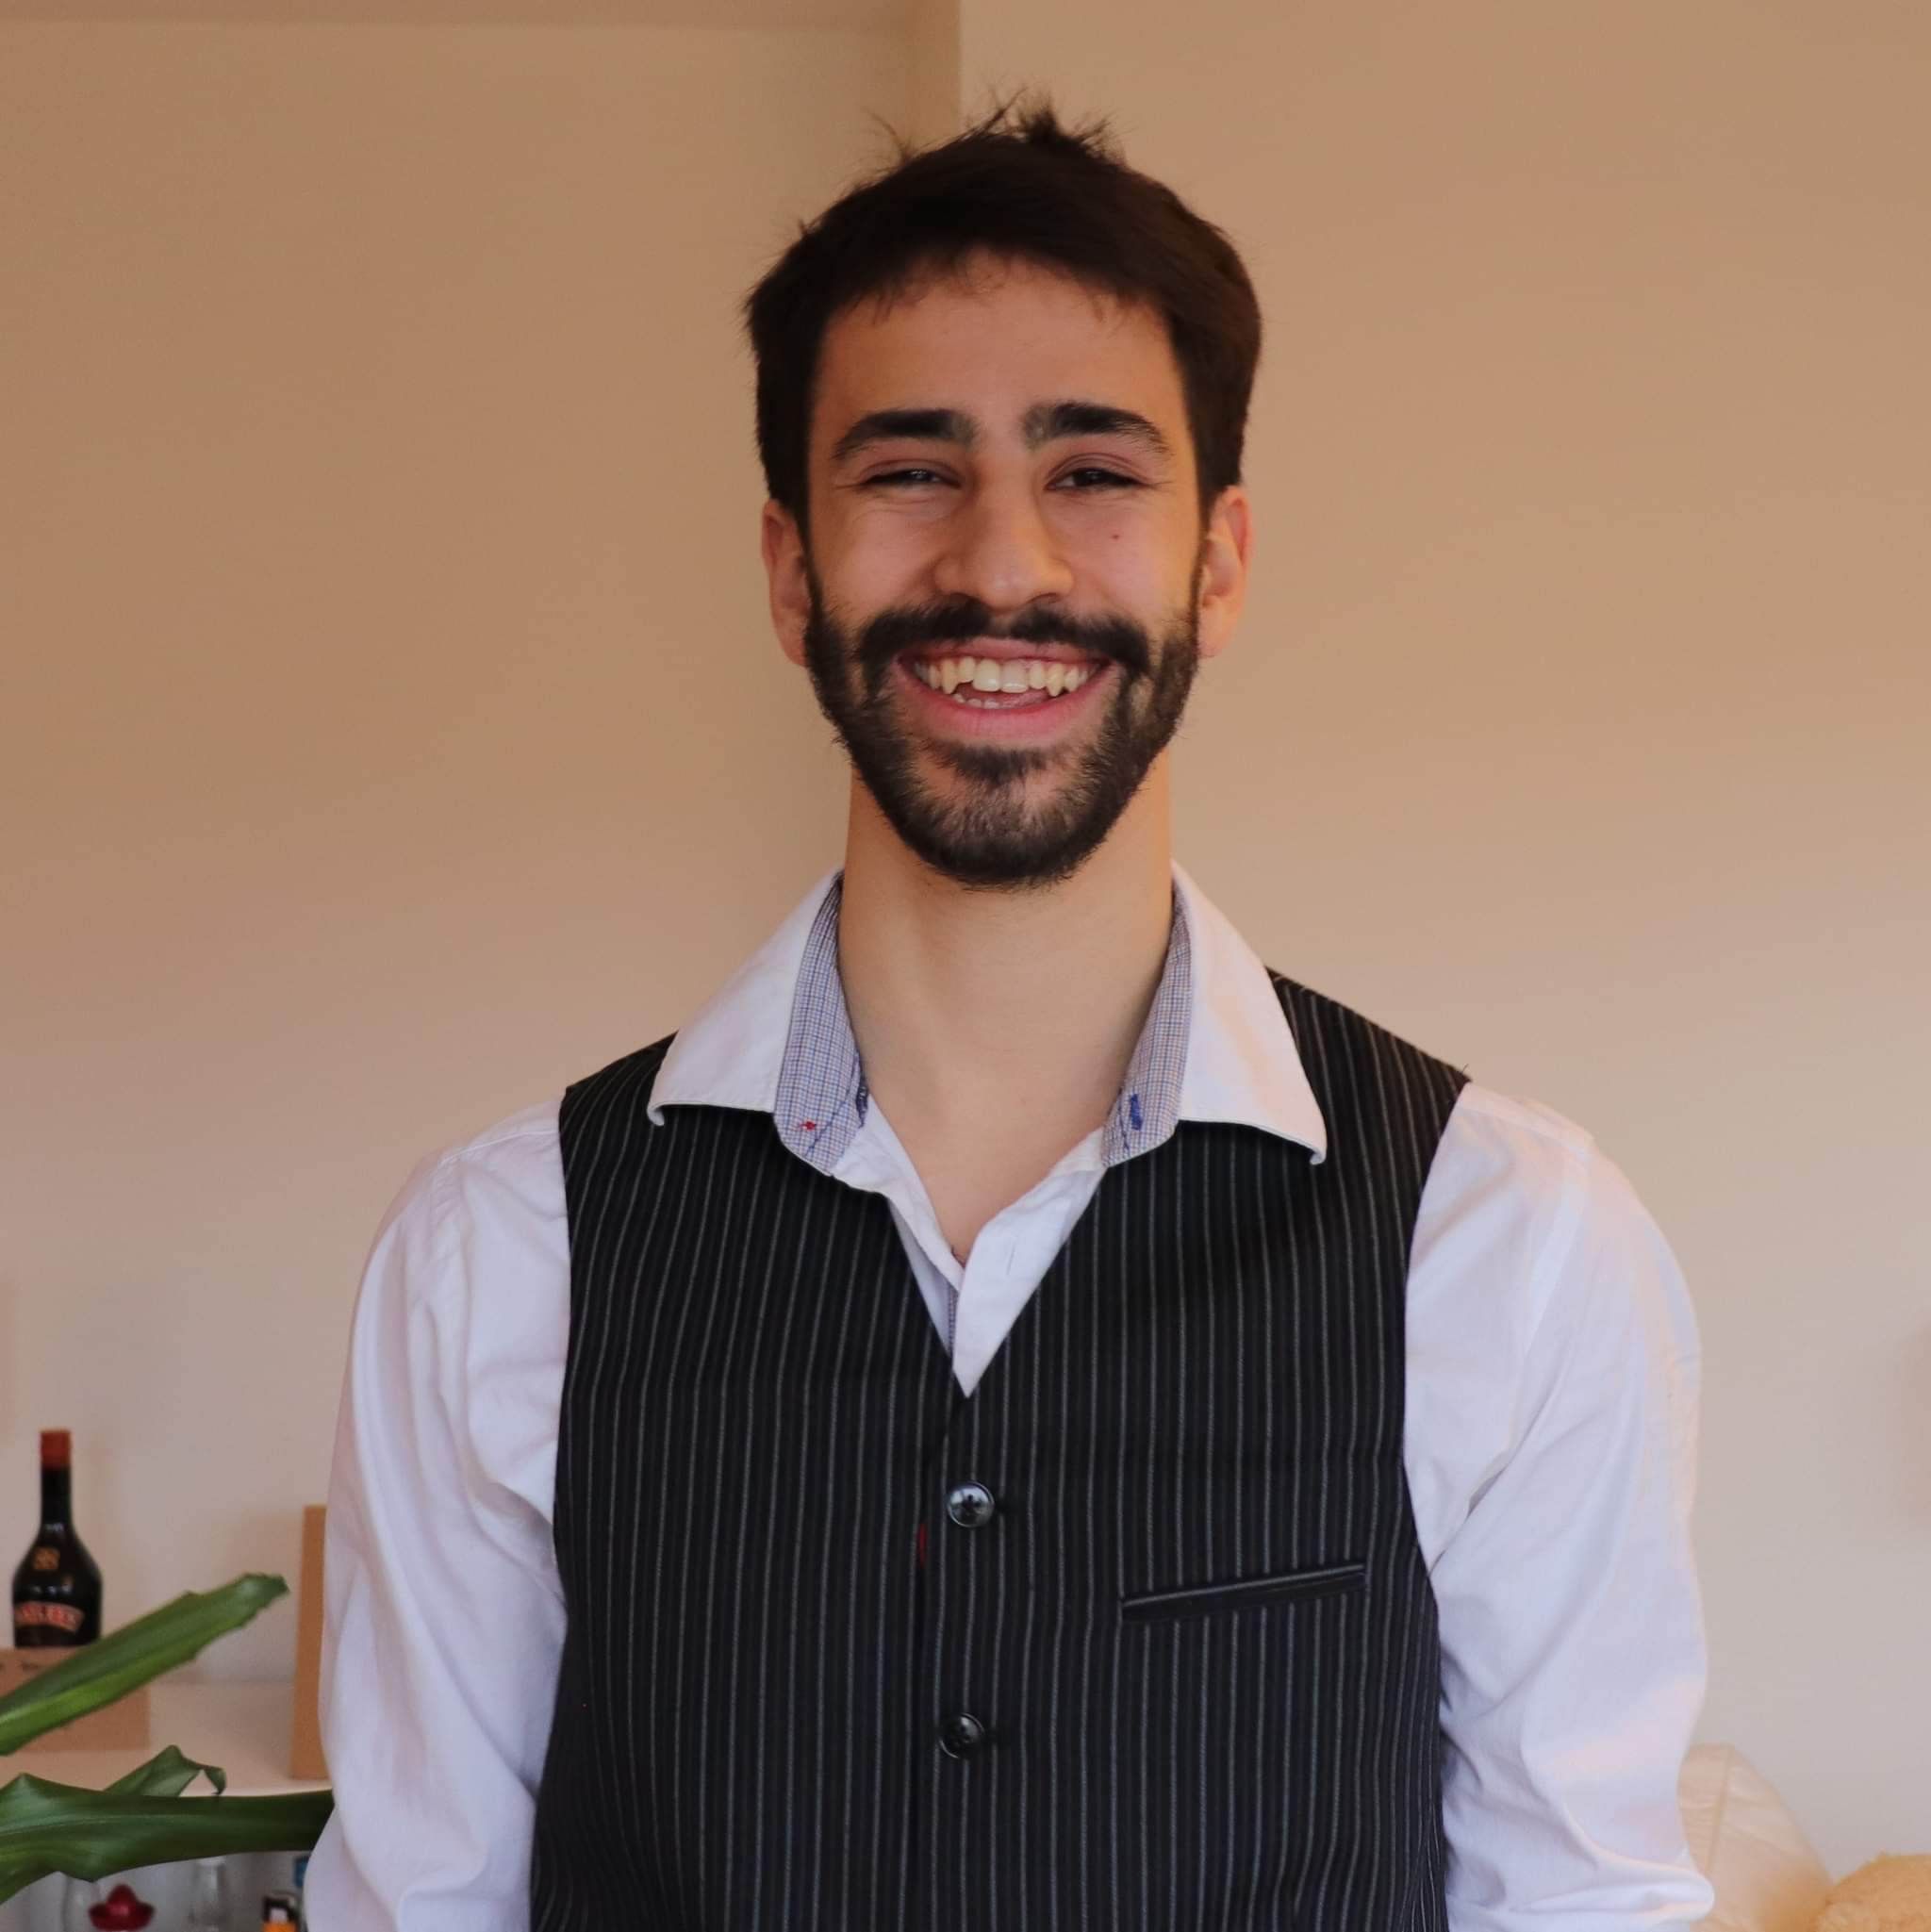
\includegraphics[width=0.8\textwidth]{Goodlooking}
    \caption{Candid picture of the author, Karim Bouzid.}
    \label{fig:Goodlooking}
\end{figure}
I would like to thank those persons close to my heart that make my life a paradise on Earth. It would not have been possible if not for the invaluable support and love of those close to me. To them I say a heartfelt thank you! And I'd like to congratulate you, who is currently reading this, for interesting yourself in a subject that will deeply impact the wellbeing of generations to come, especially considering how "nothing is received with so much reluctance as instruction". \par
\vskip \baselineskip
I dedicate this memoir to my dear friend Frédéric Langlois.
}
\epigraph{
    This memoir is written for those who will eventually benefit from it. 
    \vskip \baselineskip
    \textit{"Like rowing a boat,} \par
    \textit{We enter the future backwards.} \par
    \textit{All we see are the scenes of the past,} \par
    \textit{And no one cannot see the views of tomorrow."} \par
    \vskip \baselineskip
    A better future lies beyond the horizon through our individual actions. Despite the obstacles one faces when rowing toward a far away goal, it is important to remember that where one currently stands matters not as much as where one strives toward.
}

\usepackage{doi}
\usepackage{xurl}
\hypersetup{bookmarksnumbered,
            unicode,
            linktoc=all,
            pdftitle={\thesistitle},
            pdfauthor={\thesisauthor},
            pdfsubject={},                                % Add subject/description
            pdfkeywords={Impedance, Microorganisms, Microfluidics, Bioinstrumentation, Electronics, Signals, Processing},
            pdfborder={0 0 0}}
% See https://github.com/k4rtik/ucetd-latex/issues/1
\makeatletter
\let\ORG@hyper@linkstart\hyper@linkstart
\protected\def\hyper@linkstart#1#2{%
  \lowercase{\ORG@hyper@linkstart{#1}{#2}}}
\makeatother

\begin{document}
%% Basic setup commands
% If you don't want a title page comment out the next line and uncomment the line after it:
\maketitle
%\omittitle

% These lines can be commented out to disable the copyright/dedication/epigraph pages
\makecopyright
\makededication
\makeepigraph


%% Make the various tables of contents
\tableofcontents
\listoffigures

\acknowledgments
I would like to thank my two incredible professors for their support and guidance throughout my MSc, Professor Benoit Gosselin and Professor Sandro Carrara. I would also like to thanks the numerous persons that helped me these last two years. Martin Gagnon of the technical service provided me with countless advices and technical supports. Gabriel Gagnon-Turcotte and Partha Sarati Das acted as true mentors during my research. My fellow students of the Biomedical Microsystems Laboratory Mohamad Feshki, Vahid Khojasteh, Mohammad Makhdoumi Akram, Saeed Ghaneei-Aarani, Michelle Janusz, Félix Chamberland, Magali Ozon, Mousa Karimi, Simon Tam, Nazilah Hosseini, and  Quentin Mascreet. Fellow students from the EPFL Gian Luca Barbruni and Leonardo Iannucci. And finally my brother Sami Bouzid who inspired me to pursue research in the field of electronics. 
\abstract
To this day, a couple of biosensors have been proposed to quickly and easily measure the features and properties of individual microrganisms members of an heterogeneous population, but none of these approaches were adequate candidates to perform measurements directly in the field. Biosensors for micron-scale organisms generally require extreme sensitivity or specificity, which are difficult to combine with a portable general device. This study proposes a device based on Impedance Flow-Cytometry that can detect and quantify the size and velocity of microbeads of size bigger than 50 µm, while boasting a low cost, low size, low power, and simplicity of design and operation utilizing the potential of 3D-printing and industrial PCB fabrication. An example is provided for a Big Data application from a sampled dataset containing 2380 detected microbeads of sizes between 50 µm and 90 µm. 

\etdFrontMatter{Résumé}
À ce jour, quelques biocapteurs ont été proposés pour mesurer rapidement et facilement les caractéristiques et les propriétés des microrganismes individuels membres d'une population hétérogène, mais aucune de ces approches ne s'est avérée être adéquate pour effectuer des mesures directement sur le terrain. Les biocapteurs pour les organismes microscopiques nécessitent généralement une sensibilité ou une spécificité extrême, qui sont difficiles à combiner avec un dispositif général portatif. Cette étude propose un dispositif basé sur la cytométrie de flux d'impédance qui peut détecter et quantifier le diamètre de microbilles de tailles supérieure à 50 µm, tout en présentant un faible coût, une taille réduite, une basse consommation de puissance et une simplicité de conception et d'opération qui utilise le potentiel de l'impression 3D et de la fabrication industrielle de circuits imprimés. Un exemple est offert afin de démontrer les capacités du capteurs pour de larges échantillons, avec un jeu de données contenant 2380 microbilles détectées de tailles entre 50 µm et 90 µm. 

\mainmatter
% Main body of text follows

\chapter{Introduction}
One of the key goals of this thesis is to conceive a novel biosensor that could successfully detect and characterize microorganisms, microparticles, and compounds directly in their own natural habitat. Indeed, no such devices is universally recognized yet, and many environmental pathogens of global significance are still invisible to the scientific community per lack of adequate sensors to discover them \cite{Hutchins2019}. To that end, a portable and autonomous biosensors that could continuously monitor environmental and target-specific parameters must be designed to monitor environmental changes and their effects on microorganisms. Such real-time monitoring sensor could provide important insights into the dynamical biochemical processes that take place in biofluids and soil samples, monitor the quantity of microorganisms in an environment, and potentially identify new significant microorganisms in previously unattainable zones \cite{Kim2019,Hutchins2019}. \par

\chapter{Microorganisms, taxonomy, and cataloguing}
How exactly are microorganisms supposed to be classified? Is there a consensus in the microbiological community about a methodology considered optimal to classify between microorganisms? The short answer is no. Microorganisms are notoriously difficult to classify, primarily because so little is known about them in the first place per lack of adequate tools and sensors to characterize them \cite{Hutchins2019}, and per the huge amount of time currently required to study them. \par

Any system of scientific classification or cataloguing of things lies under the assumption that there exist an order or system of similarities in nature which can be attained by investigation \cite{Sneath1957}. The science of classification exists to quantify how much a given object A is more or less similar to a second object B than a third object C, and then strives to group these objects accordingly. Now, one first logical way to do this would be to inquire upon the tangible features of an object and group it with other objects that present these very same features \cite{Sneath1957}. But then another challenge arises: how are we to weight these features? In other words, how do these features correlate with members of a same group? Since that knowledge is unknown a priori, classification becomes a problem of correlating features present in certain objects then creating groups that are thought to fit the known objects at the time, then updating the groups and the weights when confronted with conflicting additional data. \par

For animals, some features might be easily discarded. For instance, the weight, the height, the color, the sex, etc. tell us nothing to discriminate between species: this is because those properties are uncorrelated; their knowledge does not lead to any other features of the animal \cite{Sneath1957}. From this example, it is obvious that some features are more important than others, but how can this be applied to classification in microbiology, which is still a relatively new science? Can such features as the size, morphology, composition of the membrane, color, sexual lifecycle, metabolic lifecycle, interaction with substrates, composition of the cytoplasm, presence of specific proteins or lipids, motility, or behavior be considered more important than others? Because before having proved that any feature is more important, their weights should be initialized equally \cite{Sneath1957}. With that in mind, let’s have a better look at how exactly microorganisms will be defined in this study. \par
\begin{figure}[ht]
    \centering
    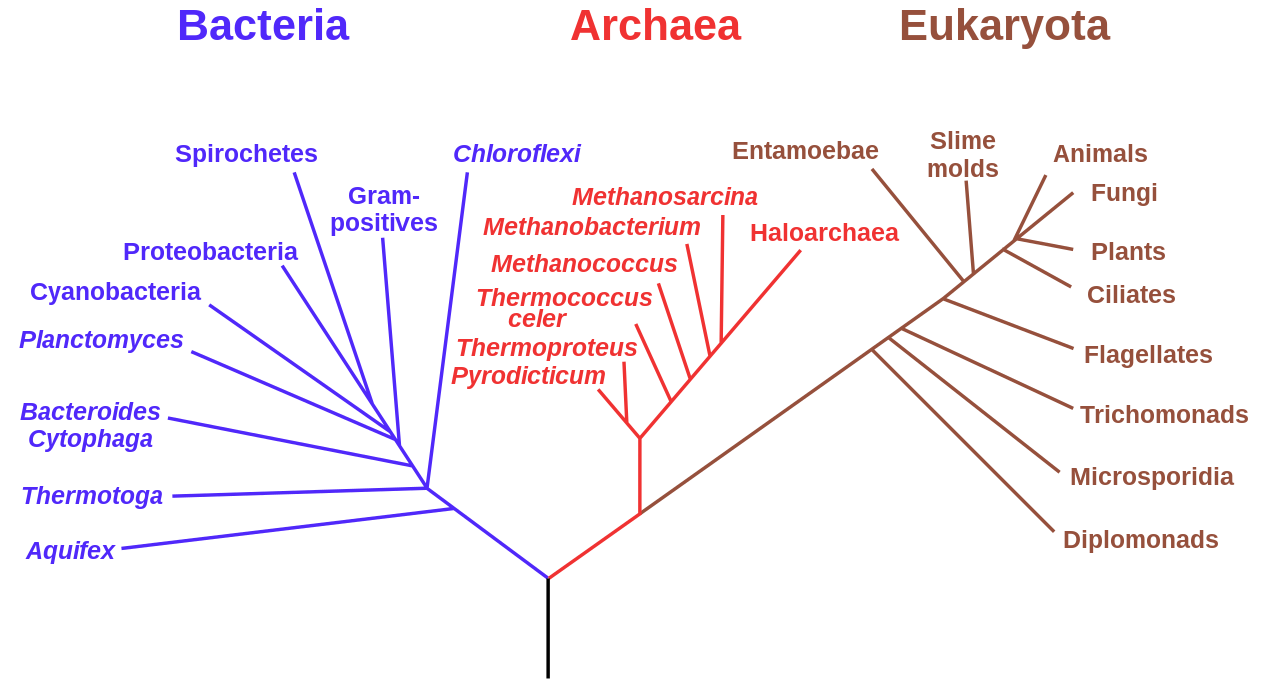
\includegraphics[width=1\textwidth]{DomainsLife}
    \caption{The 3-domains of life featuring Bacteria, Archae and Eukaryota. System of classification proposed by Carl Woese of the University of Illinois in 1990.}
    \label{fig:DomainsLife}
\end{figure}

Microorganisms generally include all living unicellular organisms which cannot be observed with the naked eye. The eyes have trouble distinguishing objects smaller than 200um, meaning that almost all single-celled organisms of the three domains of life are included in this definition. For the purpose of this study, multi-cellular organisms of dimensions below 200um will also be considered as microorganisms. Those include bacteria, archea, fungi, algae, protozoa, plankton, micro-animals such as the subphylum Myxozoa, and members of the Chromista. Those microorganisms inhabit varied environment and are parts of diverse ecosystems which made them evolve extremely diversified features. Hierarchical organization of microorganisms is often found in nature: individuals grouped together form populations (or guilds if they are metabolically related), sets of interacting guilds form communities, and different communities in a specific biotic (macro-organisms such as plants and animals) and abiotic (pH, temperature, inorganic, and organic nutrients) environment form ecosystems \cite{Hutchins2019}. It is by inferring on these varied features and by monitoring the environmental parameters that the microorganisms can be adequately catalogued. Though one practical problem arises for the standardization of tests, as microorganisms thrive in different environmental conditions. Should the tests for different microorganisms be performed at the same environmental conditions, or should they be performed at the optimum thriving condition of the specie? Species behave differently in function of the environmental parameters, and time is lacking to adequately test every specimen under a spectrum of varying environmental conditions. In this case, \citep{cowan1956ordnung} suggested that tests procedure be standardized at a unique environmental condition, since the risk of the tests being unrepeatable seem more important than the risk of the test being vitiated \cite{Sneath1957}. \par

As an example of microorganism cataloguing, bacteria can be differentiated based on the chemical composition of their cell walls. Some bacteria, called Gram-positive, feature a cytoplasmic membrane composed of a lipid bilayer, with a peptidoglycan layer of crosslinked peptides and sugars hidden beneath, beside a large concentration of teichoic acid \cite{Kocanda2014}. Gram-negative bacteria also have a lipid bilayer but have a thinner peptidoglycan layer on top of a second lipid bilayer linked to lipopolysaccharides. Gram-positive bacteria can be observed easily under a scanning electron microscope (SEM) by staining the cell walls with dye. Some bacteria species can be associated with specific chemical structures, like Staphylococcus, Streptococcus, Bacillus, Corynebacteria, Listeria, and Clostridium which all exhibit teichoic acid. The impedance of chemical compounds that compose microorganisms are found to exhibit notable signature that can help in differentiating them. Aliphatic compounds such as lipids and straight-chain alkanes, and organic acids and alcohols that contain ionizable protons are slightly polarizable in unique ways, which make them behave differently under a time-varying electrical fields \cite{Kocanda2014}. Studying these structures is thus found to be primordial to understanding and differentiating microorganisms.\par

A second logical system of classification would be using phylogenetic networks produced on the basis of sequenced genes or genomic data \cite{kapli2020phylogenetic}. This is the most popular system of classification for prokaryote, although it is more of an operational one. Single-cell organisms could be catalogued based on their DNA-DNA re-association. \citep{konstantinidis2005genomic} defines “two strains as being of the same specie when their purified genomic DNA show at least 70\% hybridization, which is equivalent to $94\%$ average nucleotide identity at the whole genome scale”. Species containing similar conserved sequences can then be linked together. Other methods with arbitrary threshold exist. For instance, several studies also define the identity of bacteria from highly conserved prokaryotic genes by sequencing their 16S ribosomal RNA gene (rDNA). Using these universal prokaryotic primers results in reliable and inexpensive taxonomic classification, but favors bacteria over archae, resulting in an under-estimated diversity and taxonomic resolution of archae \cite{Horve2020, Xu2006}. \par

Gene sequencing also suffers from important limitations. Contrarily to what is expected, the networks produced in such manner do not necessarily represent accurately the evolutionary history of the species member. Noise may affect and corrupt the sequencing \cite{kapli2020phylogenetic}. Moreover, the analysis may be troubled by horizontal gene transfer, gene recombination, convergent evolution of similar features, or hybridization between species situated far from each other on the tree. Great care should also be taken when creating phylogenetic trees from a single type of character - such as a protein or gene - since the genomic data represent the phylogeny (history) of that specific character, and not of the whole taxa \cite{kapli2020phylogenetic,Nosenko2013}. Serious phylogenetic studies therefore use data from multiple characters (mitochondrial, nuclear, etc.) from a single taxa in order to reduce the chance of homoplasy (false homology) \cite{kapli2020phylogenetic,Nosenko2013}. All these limitations lead to errors such that common species might be considered separated, or vice-versa. As with any set of data, falsification of previous research might also be induced by more recent studies made with optimized research instruments \cite{kapli2020phylogenetic}. \par

It is important to mention that phylogenetic networks made from genomic data do not translate adequately to the ones used in the animal and plant kingdoms, which are based on common traits. For instance, using it on animals would result in all primates (gorillas, chimpanzees, gibbons, orangutans, and humans) being of the same species \cite{Xu2006}. Instead, the biological species concept is currently the most popular one for sexual organisms possessing a meiotic life cycle, such as the vast majority of plants, animals and sexual eukaryotes. The choice of classification system is still now in evolution, this explains the numerous modifications in the species concepts observed for prokaryote and eukaryote in the scientific community \cite{Xu2006}. \par

The state of the art for scientific classification of prokaryote being phylogenetic networks, grouping microorganisms based on physical features should be called cataloguing, as opposed to proper scientific taxonomy, as it is effectively used only as a parallel approach to find tangible feature-keys for identification \cite{Sneath1957}.

\chapter{Biosensors}
\label{chap:Biosensors}
A biosensor is defined as “an analytical device, used for the detection of a chemical substance, that combines a biological component with a physicochemical detector” \cite{turner1987biosensors}. A biosensor is a self-contained apparatus that interacts with a specific bioreceptor (e.g. enzyme, antibody, DNA, proteins, etc.) taken from a given analyte (e.g. tissues, cells, polluted water, soil, etc.) using a physicochemical transducer. The transducer translates the electrochemical changes taking place in the analyte that modify the parameters of the bioreceptor into a useful signal (generally electrical or optical) that can be sampled by electronical circuits \cite{Kim2019}. Biosensors can be used to monitor a broad range of biorecognition events or be engineered to target specific ones. The transducer can be of an electrochemical (amperometric, potentiometric, impedimetric, and conductometric), optical, electrical, gravimetrical, pyroelectrical, or piezoelectrical nature. Current, voltage, resistance, capacitance, permittivity, light scattering, mass, and temperature, among others, can all be measured as a function of time - or as a frequency spectrum - to monitor bio-electrochemical reactions. The specificity and sensitivity of the biosensor depends on the detection mechanism, the way the bioreceptor is interacted with, and the type, shape, and size of the transducer \cite{Maas2018}. \par

Unlike laboratory-based biosensors, those designed for portable applications can be affected by harsh and fluctuating environmental conditions for prolonged duration in unsupervised environments. These biosensors can consequently be affected by shortcomings such as a gradual biofouling at the analyte-sensor interface, a limited stability of numerous bioreceptors, changing environmental conditions which can denature the obtained results, and an inefficient interaction between the sample and the sensor. The biofouling is characterized by an accumulation of proteins, cells, or macromolecules through unspecific binding on the sensor’s surfaces. This adsorption hampers the target analyte’s diffusion to the sensor’s surface and gradually decreases the sensitivity and performance over time. The variation in environmental conditions (such as temperature, pressure, humidity, pH, etc.) modifies the regions of operation of the device. An active calibration is required to consider these parameters, which is time and resource consuming. The interfaces that constitute these biosensors are paramount to the performances of the device, considering the heterogeneity of biological elements \cite{Kim2019}. Tissues, for example, are constituted of different cellular layers with differing biochemical markers; soils are constituted from an aggregate of inert molecules, particles, microorganisms, etc.; water is a biofluid in which flows minerals, inert particles, microplastics, microorganisms, etc. The specificity of the biosensor should thus be sufficient to measure the desired analyte in place of the other components, or alternative solutions should be erected to compensate this lack. \par

The first general design constraints \cite{horowitz1989art} defined at this point of the study concerning the fabrication of the biosensor to study microparticles are:

\begin{itemize}
	\item Portability. The system is targeted for uses in situ directly in the fields.
	\item Online and offline monitoring. The system should monitor and trace important parameters in real-time when needed and store them in memory for further offline post-processing.
	\item Simplicity. Complexity in electronic systems is usually associated with an increase in power-consumption and noise magnitude. Keeping it as simple as possible will allow the system better performances and ease of use. 
	\item Affordability. Ideally, the system will be widely used to gather macroscopical data about microorganisms unknown to date. A low-price is thus required for such a large scall implementation. 
	\item Robustness. It should be possible to use the system in harsh conditions of temperature and humidity, in the presence of contaminants, dusts and dirt, with little to no modifications needed for the bio-sample, and for lengthy periods of time.
\end{itemize}
\section{Impedimetric sensors}
Following the requisites enumerated in \autoref{chap:Biosensors}, a sensor based on the measure of impedance seems to be ideal. Impedimetric sensors are generally simple and affordable, portable, robust, and permit measurements on the fly and digital storage to memory. \par

Impedance sensors can be separated in two categories: resistive sensors and capacitive sensors (see \autoref{app:CapacitanceBiosensors} for a short literature review of Capacitance biosensors, which was also published as a section in the soon-to-be-published "A Comprehensive Review of Advances in Electrochemical Biosensors for Microbial Monitoring" by Seyedeh Nazila Hosseini. Some parameters are notable when designing such sensors, such as the detection principle, the resolution, delays, response time, dynamic range, excitation frequency range, sensor and electrodes size, linearity, number of channels, precision, input waveform, and power dissipation \cite{Carminati2017}. The change in impedance can be caused by a variation of the materials resistivity, dielectric constant, or geometry. The resistivity and dielectric constant depend on the mobility and quantity of charge carriers in the material. Electrons in metals and semiconductors, photoconductor, and ions in electrolytic solutions are examples of change to the number of charge carrier, whereas temperature variations can instancy the change to the mobility of charge carrier \cite{Carminati2017}. An ideal sensor would maximize the time response, the dynamic range, the excitation frequency range, the linearity, and the precision of the measurements; while minimizing the delay times, the size of the sensor and electrodes, and the power dissipation. \par

An impedance is defined from the complex Ohm's law \cite{leHuy2004circuits} based on the ratio of a voltage signal to a current signal : 
\begin{equation}
   Z(j\omega) = \frac{V_{in}(j\omega)}{I_{out}(j\omega)} = \frac{V_{out}(j\omega)}{I_{in}(j\omega)} = \frac{V_m}{I_m} \times e^{-j\phi} = \lvert Z \rvert e^{-j\phi} = \Re(Z) +j \times \Im(Z)
   \label{eq:ImpedanceEIS}
\end{equation}
Where $Z$ is the impedance, $V$ is the applied (or measured) voltage, $I$ is the measured (or applied) current, $\phi$ is the phase difference between the voltage and current, $\omega$ is the angular frequency, and $j$ is the imaginary unit value. \autoref{fig:VoltageCurrent} describes some of these parameters. \par
\begin{figure}[h]
    \centering
    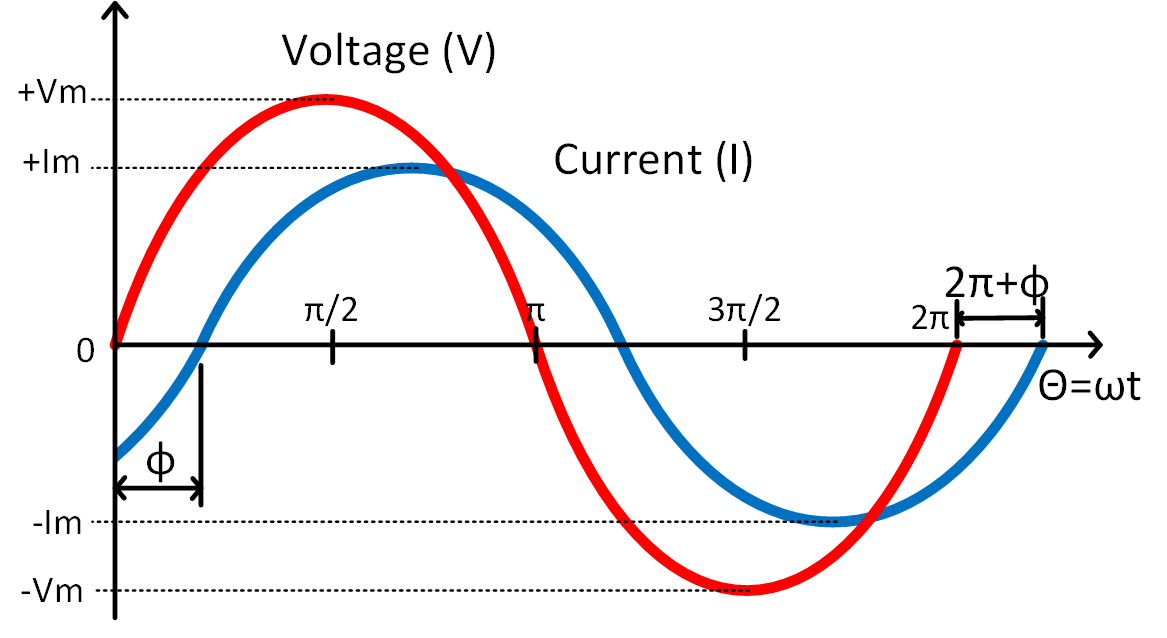
\includegraphics[width=0.7\textwidth]{VoltageCurrent}
    \caption{Current and voltage sinewaves.}
    \label{fig:VoltageCurrent}
\end{figure}

When considering current and voltage signals constituted only of sinusoids of the same frequency, an analytical representation can be used to simplify the mathematics involved and represent the values as phasors. Phasors are complex representations and can thus be represented in a 2-dimensional plane as a function of their real and imaginary components for rectangular forms, or magnitude and phase for polar forms (see \autoref{fig:ComplexImpedance}). The Real part of the impedance is assimilated to a resistance $R$ value, which is the component of an impedance responsable for power-dissipation. The Imaginary part of the impedance is assimilated to a Reactance $X$ value, which affects the signal without dissipating power. The magnitude $\lvert Z \rvert$ and phase $\phi$ of the impedance can be retrieved from the Real and Imaginary components using equation \autoref{eq:Magnitude} and \autoref{eq:Phase}. \par
\begin{equation}
    \label{eq:Magnitude}
    \lvert Z \rvert = \sqrt{\Re(Z)^2+\Im(Z)^2)}
\end{equation}
\begin{equation}
    \label{eq:Phase}
   \phi = \atan(\frac{\Im(Z)}{\Re(Z)})
\end{equation}
\begin{figure}[h]
    \centering
    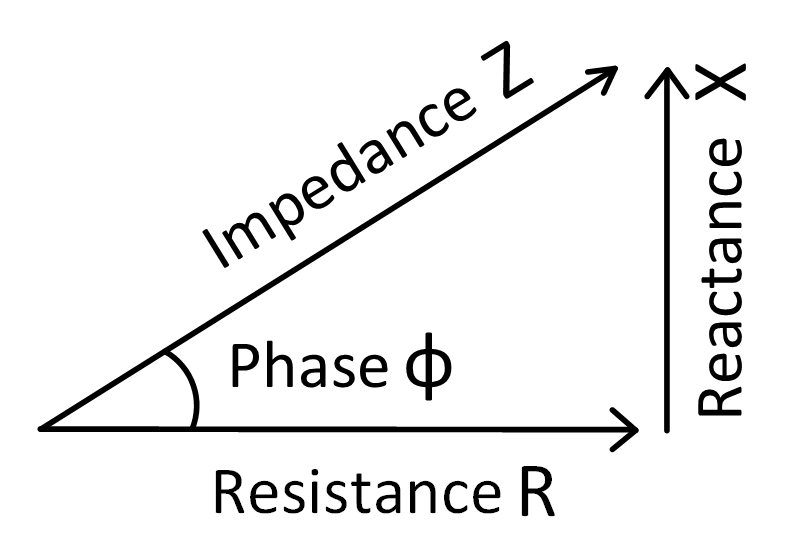
\includegraphics[width=0.4\textwidth]{ComplexImpedance}
    \caption{Impedance represented in a complex 2-d plane}
    \label{fig:ComplexImpedance}
\end{figure}
%Maybe add Impedimetric biosensor section and replace the next chapter by seomthing else
%add choice of impedimetric vs other techniques based on merit and design considerations

%CITE JESSE GREENER AND SANDRO CARRARA ARTICLES
%Research Nematodes
\chapter{Impedimetric sensors applied to biology}
\label{chap:ImpedimetricSensors}
When applied to microbiology, impedimetric techniques can be used for the measurement of whole cells, cells suspended in a solution or cells adhered to a substrate. The models for these techniques vary but they all share the same basic theory \cite{Xu2016}. One or more of the parameters found in the cell-electrolyte models is linked to its impedance. This parameter can thus be monitored from the impedance response and a flag is raised when a significant change is observed from the baseline value. This makes for a straightforward, sensitive, and quantitative detection method that is low cost, free of specialized chemicals, non-invasive, and that offers a “load and forget” experience for the user \cite{Grossi2017,Kargupta2018}.
\section{Electrochemical Impedance Spectroscopy}
\label{sec:EIS}
Electrochemical Impedance Spectroscopy (EIS) is a label-free, non-invasive technique for measuring the impedance value of an analyte in a large band of frequency \cite{Grossi2017,Sawhney2019}. EIS can be used in a plethora of applications, ranging from the monitoring of bacterial population growth \cite{Grossi2009}, to the analysis of body composition \cite{Jaffrin2008}, to the assessment of food quality \cite{Grossi2017}, metal corrosion \cite{McIntyre1996}, and battery charge \cite{diard1998eis}, to the specialized detection of cells, proteins and ions \cite{Xu2016}, to the investigation of bio-tissues non-invasively \cite{Zhang2018}. In its most basic form, EIS consists in injecting an AC sinusoidal waveform of a known voltage or current to a substance under test (SUT) and measuring its respective output current or voltage response, as shown in \autoref{fig:VoltageCurrent}. Since the amplitude and phase of the input signal is known, the impedance magnitude and phase components can then be deduced from the output response, as described in \autoref{eq:ImpedanceEIS}, \autoref{eq:Magnitude}, and \autoref{eq:Phase}. \par

Both a constant-valued voltage source and current source can be used as input for the impedance measurement, as illustrated in \autoref{fig:EIS_Galvano_potentio}. The former is termed “potentiostatic EIS” and the latter “galvanostatic EIS”. For most situation, these two techniques provide similar performance. There are, however, situations that favor one over the other, such as applications where the load voltage changes over time. Galvanostatic EIS would provide better results since the load voltage could then vary freely \cite{Grossi2017,Rajabzadeh2019EIS}. Galvanostatic EIS also benefits from an added convenience since the output is a voltage signal, which makes it easier to sample and manipulate compared to a current output.  \par
\begin{figure}[ht]
    \centering
    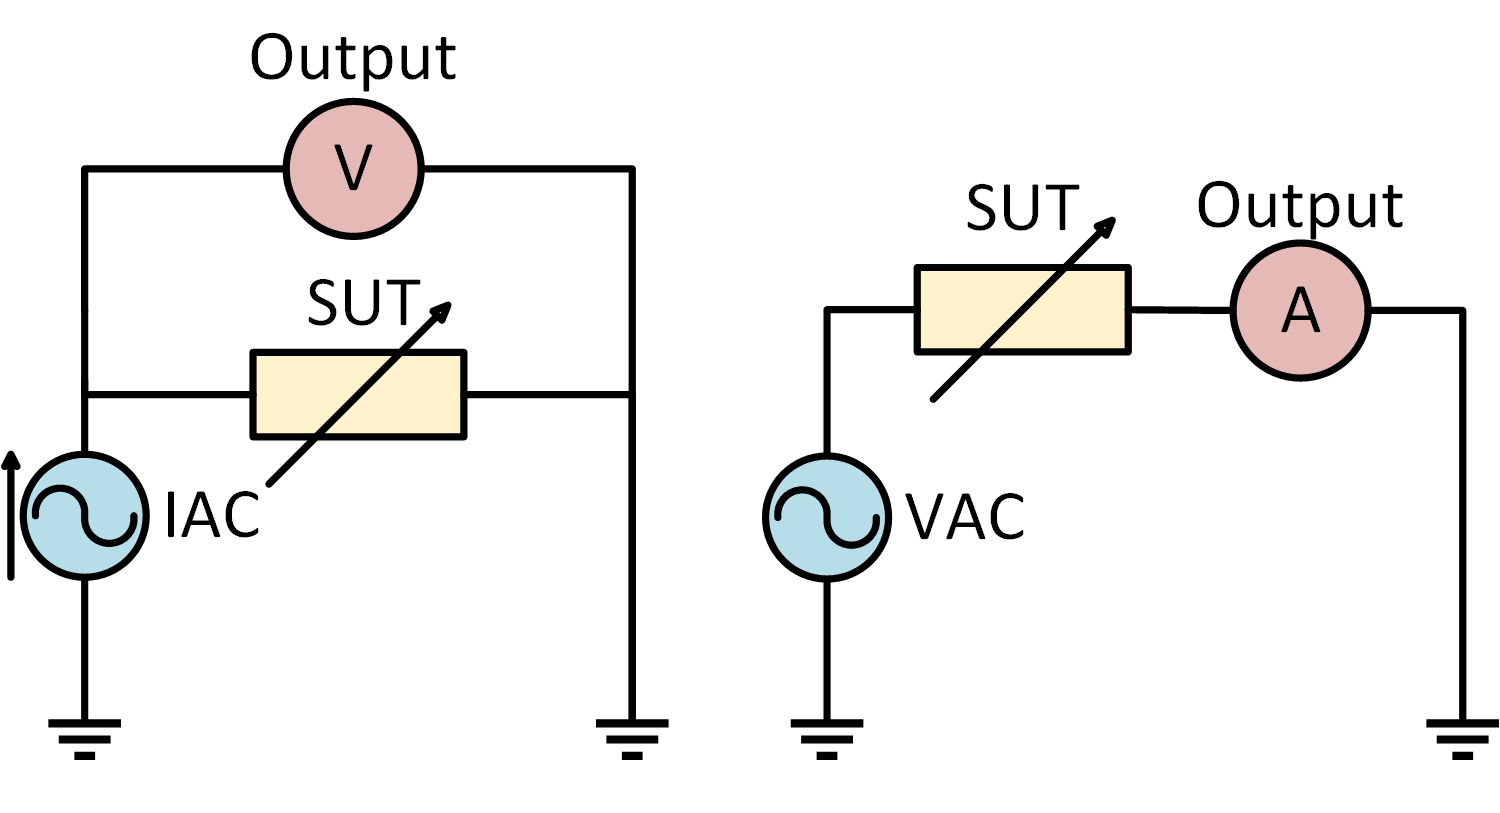
\includegraphics[width=0.8\textwidth]{EIS_Galvano_potentio}
    \caption{Galvanostatic (left) and potentiostatic (right) EIS.}
    \label{fig:EIS_Galvano_potentio}
\end{figure}

Sending sinusoidal waveforms of increasing frequency and repeatedly measuring the impedance using \autoref{eq:ImpedanceEIS} is an easy scheme for spectroscopy. This scheme results in a high Signal-to-Noise Ratio (SNR) \cite{leHuy2004circuits} but suffers from long measurement times which can be unacceptable for some applications \cite{Grossi2017,Kargupta2018,Rajabzadeh2019EIS}. This is the case since the impedance described in \ref{eq:ImpedanceEIS} is valid only for systems that have attained steady state. This means that a settling time is required before an impedance measurement can be deemed valid, to account for the transience of the system. The total transient time is a function of the system’s frequency response and the signal’s frequency. The settling time of the system itself should be low since the electronics used in its conception features fast response times (generally in the nanoseconds) \cite{horowitz1989art}. For low frequency applications, the settling time would depend mostly on the frequency of the input signal, which can be as low as a few millihertz for some applications \cite{Grossi2017}. \par

The precedent scheme can be called single-tone spectroscopy since the impedance is measured serially at fixed excitation frequencies. A higher throughput can be achieved using multi-tone spectroscopy \cite{horowitz1989art,Rajabzadeh2019Signals}. A broad-band excitation signals containing several frequency is coupled with discrete Fourier transform analysis to reduce the overall measurement time. However, additional care must be taken in order not to harm the SUT since the sum of multiple sinusoid results in a signal with a higher amplitude. In the end, the amplitude of the sinusoids at each frequency must be reduced and the phase must be chosen to minimize the Crest Factor (CF) \cite{landon1936study}. For that reason, the SNR of multi-tone spectroscopy is lower than that of single-tone spectroscopy. Rectangular pulses, Gaussian functions, sinc signals and chirp signals all are examples of such broad-band signals that can be used in multi-tone spectroscopy \cite{Grossi2017}. Pseudo random noise and Sigma-Delta Modulator ($\Sigma \Delta M$) \cite{reiss2008understanding} can also be used to produce the excitation signal; these two signals were tested by \citep{Rajabzadeh2019Signals}. The former tries to cover the entire frequency band of interest at once and the latter is a digitized variant of any analog signal such as the ones described previously. Pseudo random noise suffers from the same inconvenient as multi-tone and provides a satisfying spectrum only at the price of a high complexity; but since it is digitized, it is impervious to noise and can be multiplexed more easily. The same can be said of $\Sigma \Delta M$, it is however easier to implement and thus offers the better compromise between speed, precision, spectrum reliability and complexity \cite{Rajabzadeh2019Signals}. \par

Considering the broad range of applications permitted by impedimetric techniques, it is not surprising to find that the devices are heavily application specific. For example, the corrosion analysis of chemical coating is generally done at low frequency (a couple of hertz) \cite{Sawhney2019}, Impedance Microbiology (IM) is mostly done with a wide bandwidth that can begin as low as sub-hertz measurement and spans up to a couple hundred kilohertz, whilst whole-cell measurement is accomplished at Radio-Frequency (RF) ranging from Low Frequency (LF) to Very High Frequency (VHF) (30kHz to 300MHz) \cite{Xu2016,Opitz2019}. The impedances measured can be as low as a few milliohms and as high as tens of megaohms \cite{Grossi2017}. \par

Impedance, as described by \autoref{eq:ImpedanceEIS}, is defined for Linear Time Invariant (LTI) systems only. In order to be considered LTI, a system must respect the three conditions of linearity, stability and causality. Causality and Bounded-Input Bounded-Output (BIBO) stability are always respected for real-life systems in steady-states. However, linearity could pose a problem since most electrochemical systems are non-linear: the input signal should be of a low enough amplitude so as to operate in a pseudo-linear region (see \autoref{fig:smallEIS}) and no DC voltage or current should be added in order to minimize electrode-analyte polarization \cite{Grossi2017,Xu2016}. \par
\begin{figure}[ht]
    \centering
    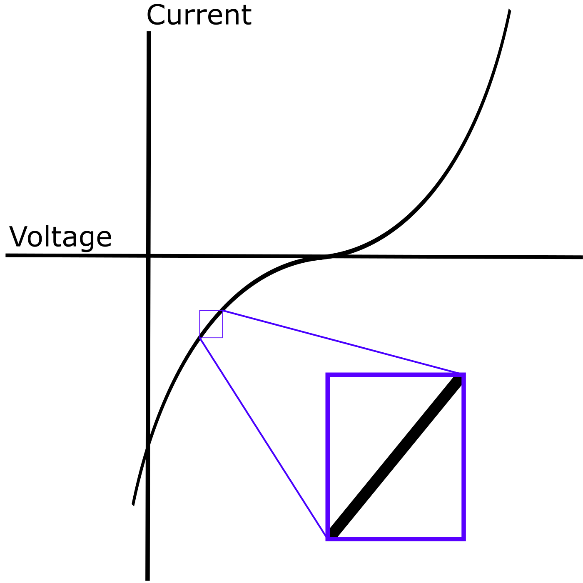
\includegraphics[width=0.5\textwidth]{smallEIS}
    \caption{Pseudo-linear region of electrochemical systems. Shows the principles of small perturbations for linear approximations.}
    \label{fig:smallEIS}
\end{figure}

To take into considerations these complicated needs, bench-top instruments such as LCR meters, Frequency Response Analyzer (FRA) and impedance analyzers offer performance extensive devices for impedimetric investigations in laboratory. These devices feature high accuracy, a broad band of available test frequency, configurations for two-, three- or four-electrodes modes (see \autoref{sec:ElectrodeDesign}) both for potentiostatic and galvanostatic EIS, and extensive software for complex modelling and data-fitting of the measured impedance. These devices are nevertheless \textbf{expensive, bulky, and energy-inefficient} which makes them unsuitable for portable measurements in the field \cite{Grossi2017,Chowdhury2017,Sawhney2019}. 
\subsection{Electric Cell Substrate Impedance Sensing}
EIS can be applied to cells bounded to a substrate to obtain better results and specificity. Electric Cell-Substrate Impedance Sensing (ECIS) uses EIS on cells adsorbed on the device’s electrodes in order to follow the cell’s activities in real-time such as the variations in shape, spreading area and tightness of adherent cells. The cell’s membrane acts as an insulator compared to the ion-rich microbial broth such that the impedance measured from the electrodes increases as the confluence of cells on the electrode is established. Confluent cells adhered to the electrode’s surface effectively reduce the electrodes’ surface area, thus offering an impedance that varies only accordingly to the cell’s shape and tightness \cite{Wegener1999,Xu2016}. At low frequency, the electrical field created by the electrode has an easier time passing through the cell’s junction, whereas at high frequency, the cell’s cytoplasm becomes short-circuited, which makes it a lower impedance path for the electrical field. These properties can finally be monitored by measuring the impedance frequency spectrum as a function of time and following its localized changes: a low frequency change corresponds to a variation in cell-to-cell and cell-to-electrode tightness; and a high frequency change corresponds to a variation in the cell’s volume or shape \cite{AppliedBiophysics}. \par

The downside of this technique is that in a heterogeneous analyte, some compounds other than the targeted microorganism can adhere to the electrode and falsify or at least denature the obtained results. To counter this, the use of antibody to increase the SUT’s specificity is prominent in ECIS. These antibodies are immobilized on the sensor’s surfaces to functionalize it for a specific biological sensing application. This action also decreases the value of the critical microbial concentration threshold $C_{TH}$, which makes it possible to detect even lower concentration of bacteria and decreases the overall Detection Time (DT) \cite{Lei2014}. The use of antibodies to increase the specificity makes ECIS a poor choice for an application that aims to identify unknown microorganisms of varying properties and sizes, despite that it is a non-invasive and label-free technique. Another shortcoming of this technique is the poor stability of the immobilized cells and the great sensitivity of the performance with the choice of the immobilization technique \cite{Grossi2017}. \par

ECIS nevertheless possesses the advantage of permitting the analysis of microorganisms on solid culture media. The SUT is dropped and let to diffuse on a solid medium in contact with the electrodes so that the microbes may adhere to them. Despite its simpler fabrication and better portability, ECIS for solid media culturation provides similar performance to liquid media \cite{Choi2009}.

\section{Single-cell modelling}
\label{sec:CellModel}
The impedance of whole cells can also be used to calculate important parameters of microorganisms. The single-shell and two-shell models generally used for the simulation of biological cells in an aqueous solution can be approximated as simple charged particles in suspension in a solution considering their relative magnitude compared to the bulk fluid \cite{Xu2016}. The simplest model for a biological cell with a lipid layer plasma membrane is the “single-cell” model \cite{asami2002characterization,Gawad2004,morgan2006single,Sun2010,Xu2016} modelled by a homogeneous phase cytoplasm and an insulating thin shell, as shown in \autoref{fig:CellModel}. Bacteria, yeast, and plant cells are examples of microorganisms that possess a cell wall outside of the plasma membrane. This addition modifies the single shell model to a double shell model. A similar kind of analysis as the single-shelled model can be done, which is described in detail in \citep{asami2002characterization} \cite{Xu2016}. Maxwell’s mixture theory can be applied to obtain the equivalent complex permittivity of the mixture following these equations \cite{Xu2016,morgan2006single}:
\begin{equation}
   \varepsilon_{mix} = \frac{\varepsilon_m (1+2\phi f_{CM})}{1-\phi f_{CM}}
\end{equation}

\begin{equation}
   f_{CM} = \frac{\varepsilon_c - \varepsilon_m}{\varepsilon_c + 2\varepsilon_m}
\end{equation}

\begin{equation}
   \phi = \frac{4}{3} \pi R^3 \frac{1}{\kappa w l h}
\end{equation}
\begin{figure}[h]
    \centering
    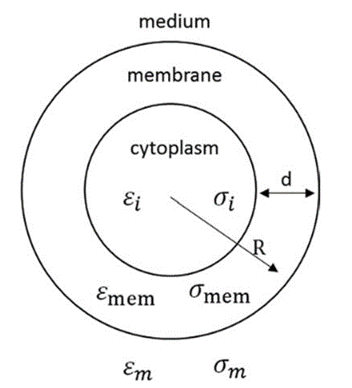
\includegraphics[width=0.4\textwidth]{CellModel}
    \caption{Electrical model of a single-shelled cell suspended in a medium. \citep{simscale_2021}}
    \label{fig:CellModel}
\end{figure}
Where $\varepsilon_m$ , $\varepsilon_c$, and $\varepsilon_{mix}$ are respectively the complex permittivity of the medium, cell, and cell-medium mixture. $\phi$ represents, the volume fraction of the cell to the detection area, $f_{CM}$ the Clausis-Mossotti factor, $h$ the height of the channel, $R$ the cell radius, $\kappa$ the cell constant, and $w$ and $l$ are the width and length of the coplanar electrodes, respectively. This equation can be used to determine the single-shelled spherical cell model, which describe the cell permittivity \cite{Xu2016,morgan2006single} $\varepsilon_c$ as :
\begin{equation}
\epsilon_c = \frac{\varepsilon_{memb} (\rho ^3 + 2 \frac{\varepsilon_i-\varepsilon_m}{\varepsilon_i+2\varepsilon_m})}{\rho ^3- \frac{\varepsilon_i-\varepsilon_m}{\varepsilon_i+2\varepsilon_m}}
\end{equation}

Where $\varepsilon_{memb}$ and $\varepsilon_{i}$ represent the permittivity of the cell membrane and cell cytoplasm, and $\rho$ describe a ratio between the membrane thickness $d$ and cell radius $R$. \par

The permittivity of the medium, membrane, and cytoplasm are fundamental properties of cells, meaning that they can be used to catalog between different species. The complex permittivity is a function that depends on frequency. The choice of the excitation signal’s frequency depends on the properties targeted by the analysis. \citep{Schwan1963} distinguished between three ranges of frequency for biological cells in suspension in a liquid, named $\alpha$, $\beta$, and $\gamma$ dispersions. Frequencies below several kilohertz constitute those in the $\alpha$-dispersion and are mostly affected by electrode polarization effects caused by the EDL \cite{grahame1947electrical}, as well as ionic diffusion. The $\gamma$-dispersion is found at frequencies above 1 GHz and behaves accordingly to the reorientation of water molecules (which are dipolar) present in the SUT \cite{Hasted1973}. The $\beta$-dispersion lies in between the frequency from the $\alpha$ and $\gamma$ regions and features a fair amount of useful information for the whole cell measurements and interfacial polarization \cite{Caselli2010}. Indeed, the impact of the EDL, the cell’s size, the cell’s membrane, and the cell’s cytoplasm are all observable in this zone, as shown in \autoref{fig:CellFrequency}. This makes the $\beta$-dispersion the zone which is generally used for impedance-based cell measurements \cite{Xu2016,Opitz2019}.
\begin{figure}[h]
    \centering
    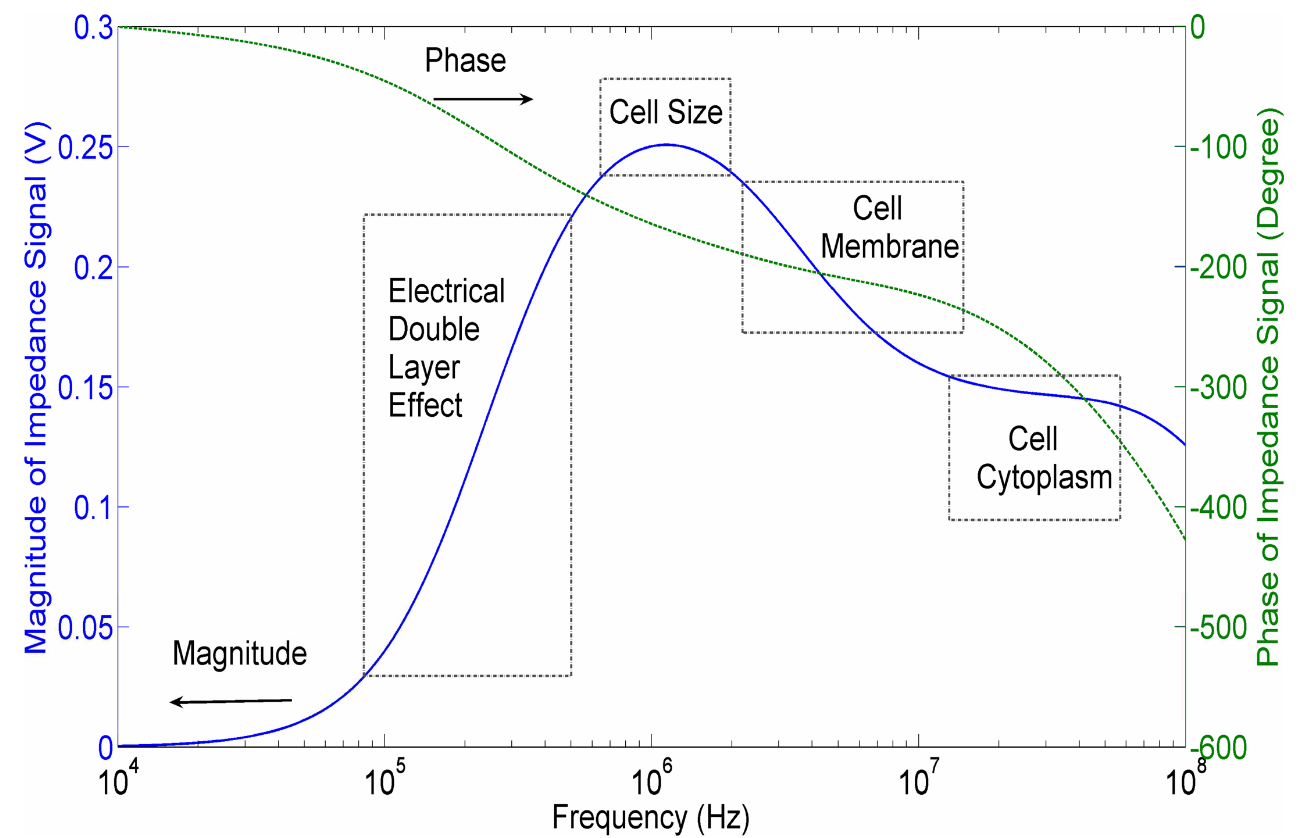
\includegraphics[width=0.9\textwidth]{CellFrequency}
    \caption{Impedance magnitude and phase variations of a single-shelled cell obtained from PSpice simulations. \citep{sun2008analytical}}
    \label{fig:CellFrequency}
\end{figure}
\section{Electrode design}
\label{sec:ElectrodeDesign}
Impedance measurements of a liquid media can be achieved with different configuration for the electrodes, termed two-, three-, and four-electrodes mode. The most basic one of them is the two-electrode implementation, which uses only two electrodes to apply the electrical stimulus and to measure its response. The signal is provided by the Working Electrode (WE) to the Counter Electrode (CE) \cite{Grossi2017} and is measured between these same two electrodes. The applied signal at the immerged electrodes creates a response in the Sample Under Test (SUT) as well as in both electrolyte-electrode interfaces. This means that the measured response is in fact not only the result of the applied signal on the analyte, but also of the two interfaces’ reactions. These are caused by the polarization of the analyte’s molecules at the interfaces in response to the difference in voltage at the junction. This effect is well-known in surface theory and is called the Electrical Double-Layer (EDL) \cite{grahame1947electrical}. \par
\begin{figure}[h]
    \centering
    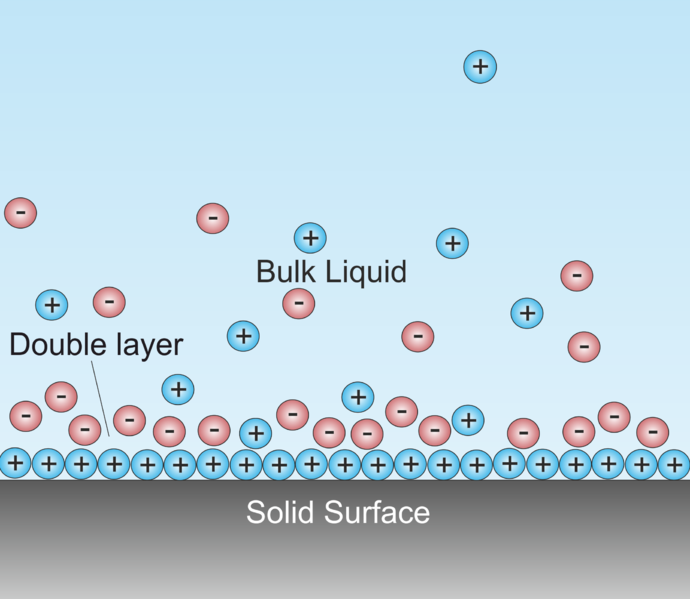
\includegraphics[width=0.6\textwidth]{EDL_image}
    \caption{Schematical view of the behavior of the charged particles at the interface between a charged conductor and an acqueous solution which forms an EDL. \citep{EDL_image}}
    \label{fig:EDL_image}
\end{figure}
The applied signal at the WE causes the electrode’s electrons to accumulate at the electrode’s boundary, as shown in \autoref{fig:EDL_image}, which induces a voltage at the electrode-electrolyte interfaces. This difference in tension causes the electrolyte’s free-moving ions to move toward the junctions, which ultimately result in ions adhering to the electrodes through chemical interactions. These adsorbed ions constitute the first of the two layers. The remaining ions are loosely attracted by the electrode’s charge via the Coulomb force and constitute the second layer, also called the “diffuse layer” \cite{grahame1947electrical}. This arrangement of charged particles creates an insulating gap which behaves similarly to a dielectric and can thus be modelled as a capacitance $C_{dl}$ in series with a resistance $R_i$.  This capacitance accumulates charges, which modifies the desired response in the case of a two-electrodes configuration. Being only a few Ångströms thick, $C_{dl}$ is usually high, in the order of a few $\mu$F \cite{grahame1947electrical}.

An exhaustive model can be used to represent the complex behavior of free-moving charged particles in the electrolyte. Firstly, the diffusion process of ions in a fluidic analyte causes the appearance of a Warburg Element, which can be approximated at high frequency to a Constant Phase Element (CPE) with a phase of 45° and a magnitude inversely proportional to the square root of the frequency:
\begin{equation}
   Z_W = \frac{A_W}{\sqrt{\omega}} + \frac{A_W}{j \sqrt{\omega}}
\end{equation}
Where $A_W$ is the Warburg coefficient, $\omega$ is the complex frequency and $j$ is the imaginary unit. A charge-transfer complex can be observed at the electrode-electrolyte interface, where kinetic exchanges of electrons create residual currents that alter the measured impedance. This charge transfer can be modelized as a resistance $R_{ct}$ Additionally, the capacitance of the EDL can sometimes be more adequately represented as a CPE \cite{gamryBasicsEIS}, following the equation:
\begin{equation}
   Z_{C_{dl}} = \frac{1}{C_{dl}} (j\omega)^\alpha
\end{equation}
Where $Z_{C-{dl}}$ is the impedance of the EDL and $\alpha$ is a constant between -1 and 1. These parameters can be assimilated to a Randles circuit \cite{Randles1947}, which is an equivalent circuit for electrochemical system made of an active electrolyte resistance $R_s$ in series with the parallel capacitance of the EDL $Z_{C{dl}}$ and series combination of the charge-transfer complex resistance $R_{ct}$ and Warburg Element $Z_W$ \cite{gamryBasicsEIS}. The Randles circuit is illustrated in \autoref{fig:EIS_fullmodel}. \par
\begin{figure}[h]
    \centering
    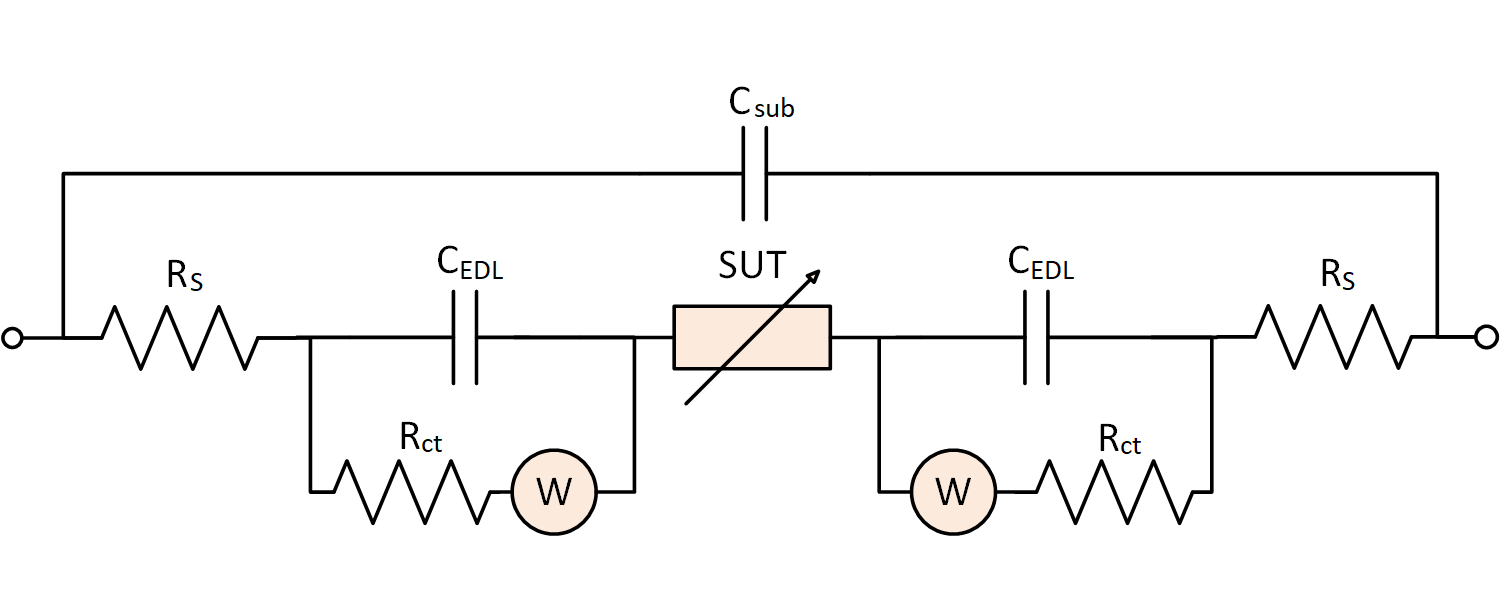
\includegraphics[width=1\textwidth]{EIS_fullmodel}
    \caption{The electrical model of an analyte in an acqueous system sampled using a two-electrode configuration can be defined by two Randles circuit.}
    \label{fig:EIS_fullmodel}
\end{figure}

With the use of electrodes made of inert material such as gold or platinum, it is possible to reduce the effect of the charge-transfer complex. It is also possible to neglect the effect of the Warburg Element with an adequate selection of the measurement frequencies since the Warburg impedance mostly affects the results at low frequency. That lower bound for the frequency depends mostly on the type and shape of the electrodes \cite{Randles1947}. With these precautions taken, the complex Randles circuit can be simplified to the model presented in \autoref{fig:EIS_simplemodel} It is important to remember that those models only superficially describe the true complex dielectric behavior seen in microfluidics for real biological cells and microparticles \cite{Gawad2004}, and that extracting the numerical values associated to these model poses quite a challenge in practice (refer to \autoref{sec:CellModel} and \autoref{sec:IFC}). \par
\begin{figure}[h]
    \centering
    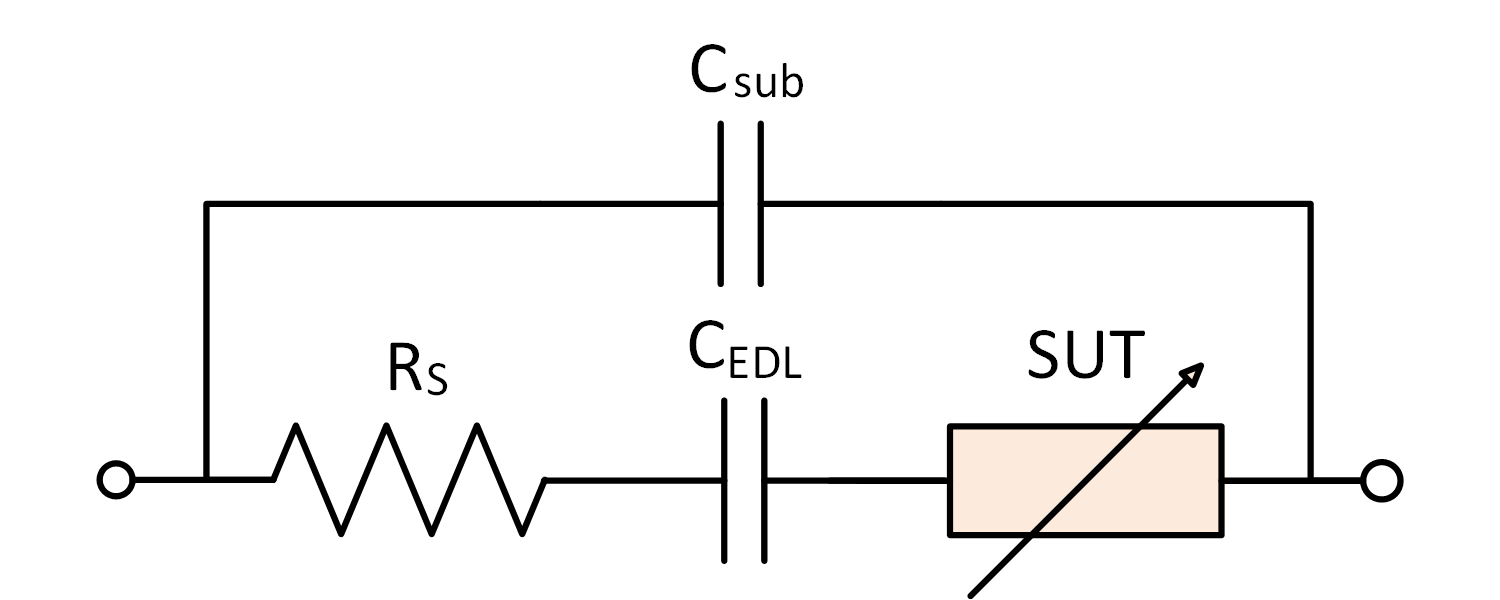
\includegraphics[width=0.7\textwidth]{EIS_simplemodel}
    \caption{The simplified electrical model of an analyte in an acqueous system sampled using a two-electrodes configuration.}
    \label{fig:EIS_simplemodel}
\end{figure}

Three-electrodes configuration uses another electrode, the Reference Electrode (RE), in order to provide a tension reference for the applied signal that is independent of the measured signal. The measurement is in this way partially dissociated from the applied signal: the measured impedance now considering only the response of the SUT and of the WE-electrolyte interface. The three-electrodes configuration offers better performance than its two-electrodes counterpart since the kinetical electrodes’ polarization is mostly an asymmetrical reaction: the charge transfer and diffusion happening at the WE are different than those happening at the CE since the difference in potential is different at the two junctions. Therefore, considering only the influence of the WE on the measured impedance gives better consistency on the results \cite{Grossi2017}. \par

Another electrode, the Working Sensing Electrode (WSE), can be added to obtain the four-electrodes configuration. In this mode, the applied signal is produced at the WE and CE and the measured signal is taken at the WSE and RE. By so doing, the measured impedance is completely dissociated of the interfaces’ behaviors since no current is drawn at either junction \cite{Grossi2017}. Using a higher number of electrodes gives more precise results at the price of complexity; thus, the choice of the number of electrodes depends on the specific application. It must also be mentioned that in some applications, the response of the interfaces can yield results just as important as the response of the electrolyte, the two- and three-electrode configurations should then not be discarded too hastily. \par

Interdigitated electrodes (IDEs) can also be used for impedance measurements. They show great promise because of their low ohmic drop, excellent signal to noise ration, robustness, and high sensitivity. They also do not need a reference electrode, which makes for a simpler implementation in a limited chip area. They are made from two separate interlocking electrodes, usually made from gold or platinum due to their biocompatibility, and inertness. The detection sensibility is usually a function of the size of the IDEs fingers; choosing smaller fingers results in a higher sensitivity \cite{Khormazard2016}.  \par
\begin{figure}[h]
    \centering
    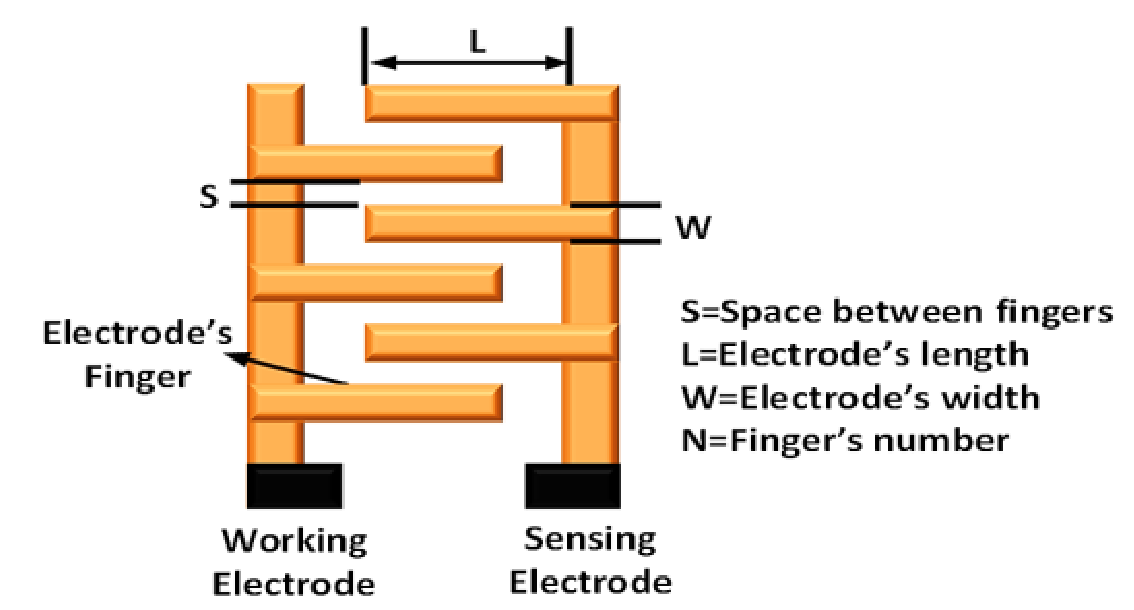
\includegraphics[width=0.8\textwidth]{Nazilah_IDE}
    \caption{Interdigitated electrodes \citep{hosseini2021optimization}}
    \label{fig:Nazilah_IDE}
\end{figure}

Faster measurement times can be achieved by using Multi-Electrode Array (MEA): a higher number of electrodes permits parallel measurements, which increase the device’s throughput \cite{Rajabzadeh2019EIS}. However, increasing the number of channels is also associated with increased digital complexity and data rates.
\section{Impedance Flow Cytometry}
\label{sec:IFC}
Impedance Flow Cytometry (IFC) is another label-free non-invasive impedimetric measurement technique. It is based on the Coulter Counter, an apparatus designed by \citep{coulter1956high} to measure the volume displacement caused by particles flowing in a fluid. It does that by monitoring the DC resistance of a liquid moving in a narrow channel only slightly larger than the size of the largest particle in the SUT, using electrodes facing each other on opposite sides of the channel. The particles act as homogeneous insulating spheres and have a finite DC resistance \cite{deblois1970counting, Xu2016,Gawad2004}. A pulsed waveform can be obtained, such as the one shown in Figure \autoref{fig:CoulterCounter}, with a transit time typically in the hundred of microseconds and an amplitude directly linked to the volume (and thus size) of the particle compared to the dimensions of the channel \cite{Carminati2017}. This is a simple and effective technique to count and size particles in a fluid. This analysis can be performed both online and offline, providing information in real-time for feedback control, or accumulated in memory for later use or post-processing \cite{david2012viability,Opitz2019}. \par
\begin{figure}[h]
    \centering
    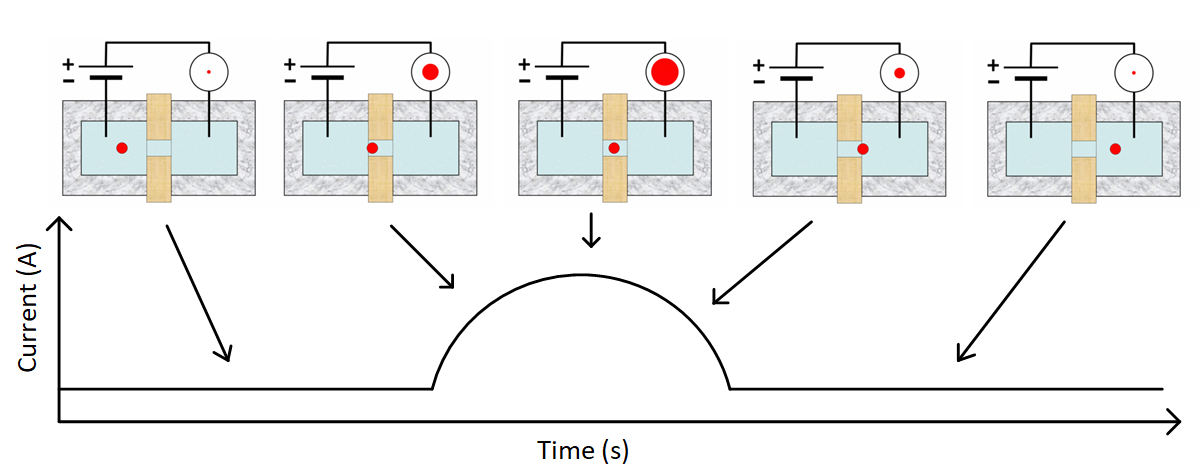
\includegraphics[width=1\textwidth]{CoulterCounter}
    \caption{Observed current response of a Coulter Counter for different particle position in the microchannel.}
    \label{fig:CoulterCounter}
\end{figure}

IFC can effectively be considered a generalization of the Coulter Counter since it measures not only the DC resistance, but the impedance value at any given frequency. When done as a spectroscopy, it leads to an adequate characterization of the dielectric properties of the cells flowing inside a microchannel, which can be used in association with their single-shell or double-shell models described in \autoref{sec:CellModel} to retrieve some important characteristics of single-celled organisms. \cite{Opitz2019, Cheung2010, Xu2016}. The complex permittivity of the mixture can be retrieved from the complex impedance knowing the geometrical parameters of the microchannel and electrodes \cite{Sun2010,Xu2016}. However, since the permittivity cannot physically be interacted with (hence it cannot be directly measure), the impedance of the mixture $Z_{mix}$ must first be acquired and converted to a permittivity using mathematical functions. As described before in \autoref{chap:Biosensors}, an impedance depends on geometrical and material factors. The complex impedance of the cell-medium system, $Z_{mix}$, can be approximated considering both the geometrical and material parameters \cite{Xu2016,morgan2006single}:
\begin{equation}
\label{eq:Zmixture}
Z_{mix}=\frac{1}{j \omega \varepsilon_{mix} l \kappa}
\end{equation}
The mathematics quickly becomes complicated here to convert from the mixture’s impedance to the mixture’s permittivity. This is the case since the volume factor $\phi$ between the cell and detection area is quite high, creating a fringing effect at the electrodes, as shown in \autoref{fig:FringingEffect}. This fringing effect could be considered inconsequential when the electric field is homogeneous and for low volume fraction cases, but that is rarely the case in IFC. Thus, the most challenging problem is how to calculate this fringing effect through the the cell constant $\kappa$, which influences both the volume fraction, and the impedance of the mixture. The Schwarz-Christoffel mapping \cite{Schwarz1869, Christoffel1867} needs to be used to calculate $\kappa$, which makes use of the complete elliptic integral of the first kind, of the complementary integral, and of the modulus of the elliptic function \cite{Xu2016,morgan2006single}. This mathematic being out of the scope of this memoir, only the mixture impedance $Z_{mix}$ will be measured in this study, and the cell parameters will be assumed retrieved. \par
\begin{figure}[h]
    \centering
    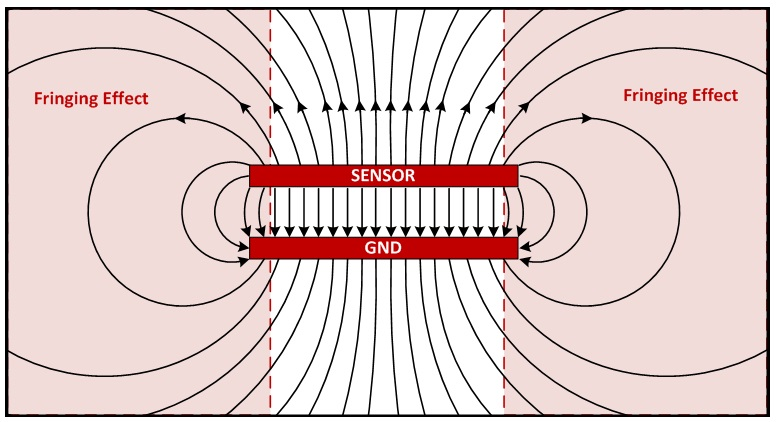
\includegraphics[width=0.8\textwidth]{FringingEffect}
    \caption{Fringing effect as modelized on parallel electrodes. \citep{FringingEffect}}
    \label{fig:FringingEffect}
\end{figure}

A simple alternative to the mathematics associated with the size determination of particles is given in \citep{De_Ninno2017,caselli2018novel}. An estimation of the particle diameter $D$ can be found with a fit to the cubic root of the measured impedance magnitude difference observed when a particle passes the electrode pairs in the channel:
\begin{equation}
\label{eq:sizeEstimation}
D = G (\lvert \Delta Z_{1} \rvert+ \lvert \Delta Z_{2} \rvert){^{1/3}}
\end{equation}
Where $G$ is a constant that accounts for a multitude of factors, including the electrode configurations, the magnitude and frequency of the excitation signal, the filter bandwidth, the channel depth and width, the electrode sizes, the EDL capacitance $C_{edl}$, the buffer conductivity, and the circuit gains. Ths constant $G$ can be determined empirically by testing the IFC system with circular beads of know diameters, then adjusting the coefficient $G$ until the diameters estimated using \autoref{eq:sizeEstimation} match the beads diameters \cite{caselli2018novel}. Such a size estimation is shown in \autoref{fig:Caselli2018DiameterEstimation}. \par
\begin{figure}[h]
    \centering
    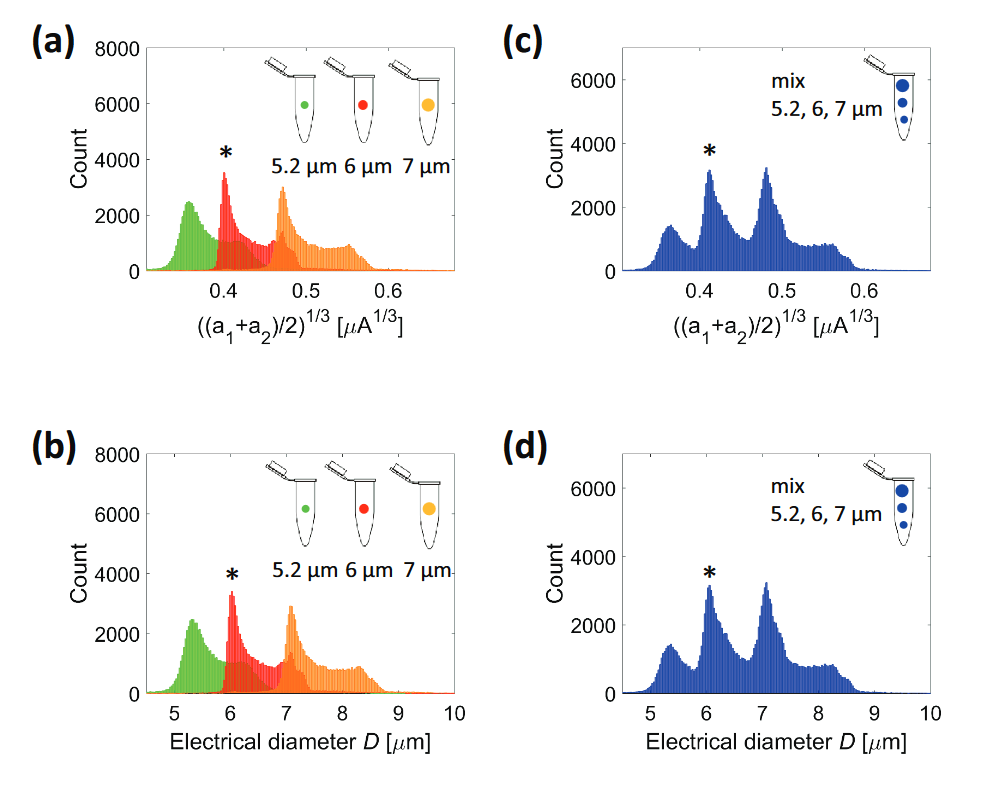
\includegraphics[width=0.8\textwidth]{Caselli2018DiameterEstimation}
    \caption{Electrical diameter $D$ estimation using equation \autoref{eq:sizeEstimation}. \citep{caselli2018novel}}
    \label{fig:Caselli2018DiameterEstimation}
\end{figure}

It is also possible to measure the particle velocity by dividing the distance between the electrode pairs $L$ with the time it took for the particle to go from one electrode to the other $\Delta t$ (which is the time difference between the two impedance maximums). Such a velocity $v$ is described as :
\begin{equation}
\label{eq:VelocityEstimation}
v = \frac{L}{\Delta t}
\end{equation}
Based on \autoref{eq:Zmixture}, \autoref{eq:sizeEstimation}, and those for whole-cell analysis presented in \autoref{sec:CellModel}, it is possible to find design parameters for the microfluidic channel and coplanar electrodes. From \autoref{eq:Zmixture}, only the volume fraction $\phi$ through the electrode width $w$, electrode length $l$, channel height $h$, and cell constant $\kappa$ (through the ratio of $w$ to $h$) can be influenced by design; the other parameters being function of the cell or medium. This means that a maximization of the volume fraction will create the maximum difference in impedance between the mixture and cell. This is intuitively correct since the cell would then replace the maximum quantity possible of mixture for the impedance measurement. Maximizing $\phi$ requires that the channel and electrodes be as small as possible. There are, however, technical limitations to the minimum size of both, which are described in \autoref{sec:FabricationMicrofluidics} and \autoref{sec:ElectrodeDesign}. To maximize the volume fraction, it is necessary to know beforehand the size of the largest particle to flow in the channel. This means that to obtain a sufficient precision for small particles, a small channel must be constructed, which will block the larger particles. This compromise means that the channel in IFC must be designed with the size of the particles in mind. The channel should be made so that the length and height of the microchannel are comparable \cite{Gawad2004}. Indeed, decreasing the length of the channel is associated with lower thermal noise. It however creates a non-uniform current density in the channel’s axis, which require further signal processing to correct the end effects \cite{Gawad2004}. A differential design is also of a prime importance in IFC to decrease the background noise and increase the sensitivity to the flowing particles \cite{Xu2016,horowitz1989art}. \par 

The electrodes size should be minimized until the impact of the substrate dielectric begins to short-circuit the frequency of interests, as a drop in precision is observed at that moment, as described in \autoref{sec:ElectrodeDesign}. Facing electrodes are a better choice for IFC than coplanar electrodes because the electrical field is uniform along the path of the particles, which greatly simplifies the mathematics associated with retrieving the cells properties from the impedance values \cite{Xu2016}. It also greatly reduces the fringing effect of the electrodes, which tends to complicate the measurement. Facing electrodes are, however, difficult to construct using lithography techniques. Coplanar electrodes being 2d structures, they can be made efficiently using a lithography mask or directly on a PCB \cite{Sun2010}. \par

These electrodes are generally fabricated with materials resistant to oxidation, such as gold or platinum. Those metals are used because of their convenience in casting for such small dimensions, for their unlimited lifetime, and since other types of electrodes such as Ag/AgCl are unsuitable for high excitation frequency \cite{Sun2010}. However, they hinder the charge exchange with the ionic solution, which causes a polarization of the ion-electrode surface, causing a double-layer capacitance $C_{dl}$ to form at the interface. The frequency must be increased beyond the EDL to access the solution resistance modulated by the presence of particles without being too affected by the EDL. For the case of gold/cell culture buffer, $C_{dl}$  is of about 0.1pF per $\mu m^2$ of electrode area \cite{Carminati2017}. One solution to reduce the EDL is to increase the electrode surface area. The throughput of IFC sensors can be improved using multiple microchannels in parallel or by increasing the number of electrodes per channels \cite{Sun2010}. \par

The frequency behaviors in IFC systems are shown in \autoref{fig:CellFrequency} and \autoref{fig:ElectrodeResponse}. For frequencies lower than 100kHz, the electrical double-layer dominates the measured impedance in micron scale electrodes, which reduces the detection sensibility of particles \cite{Xu2016,Gawad2004,Bouzid2022NEWCAS}. For intermediate frequencies (1-10MHz), the cell membrane becomes the main cause of impedance change. For higher frequencies than 10MHz, the membrane becomes effectively short-circuited, which makes the cytoplasm responsible for the variation in impedance. The impedimetric behavior of IFC sensors generally is stable from 100kHz to 10MHz. Above that, the PCB dielectric shunts the channel impedance, and the parasitics of the measurement electronics affect the results \cite{Gawad2004,Bouzid2022NEWCAS}. \par
\begin{figure}[h]
    \centering
    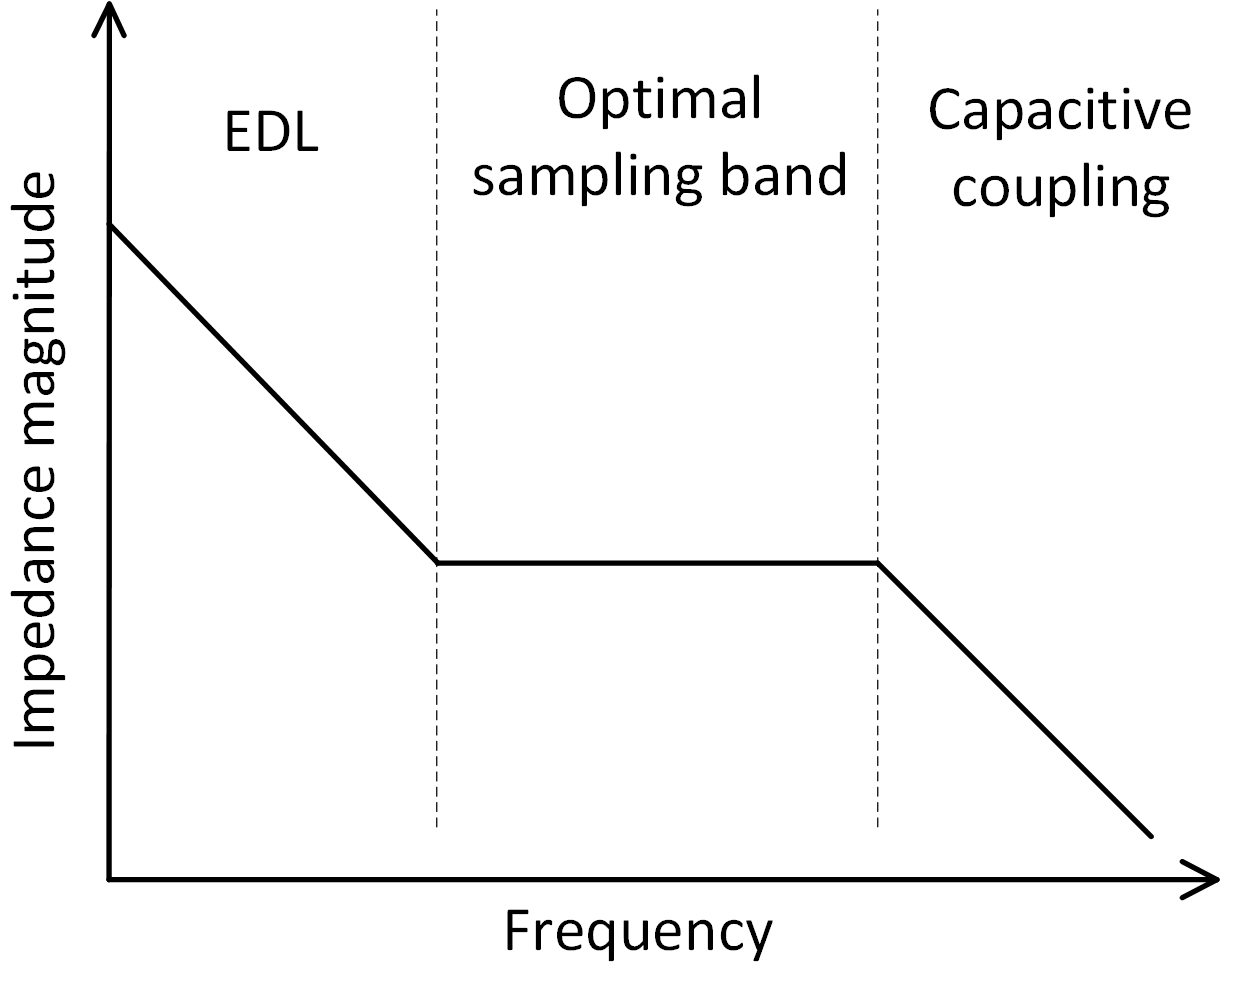
\includegraphics[width=0.6\textwidth]{ElectrodeResponse}
    \caption{Frequency behaviors observed in IFC. The optimal measurement zone is in-between the EDL and the high-frequency capacitive coupling. }
    \label{fig:ElectrodeResponse}
\end{figure}

The opacity, which is the ratio of a high frequency impedance to a low frequency impedance, is often used in particle scatter diagram in IFC. It acts as a unitless dimension for 2d-representation \cite{Xu2016}. Such type of representation can help visually differentiate or regress cell sizes and morphologies, as well as their condition or life phase. An example scattergram is shown in \autoref{fig:ScatterGram}. \par
\begin{figure}[h]
    \centering
    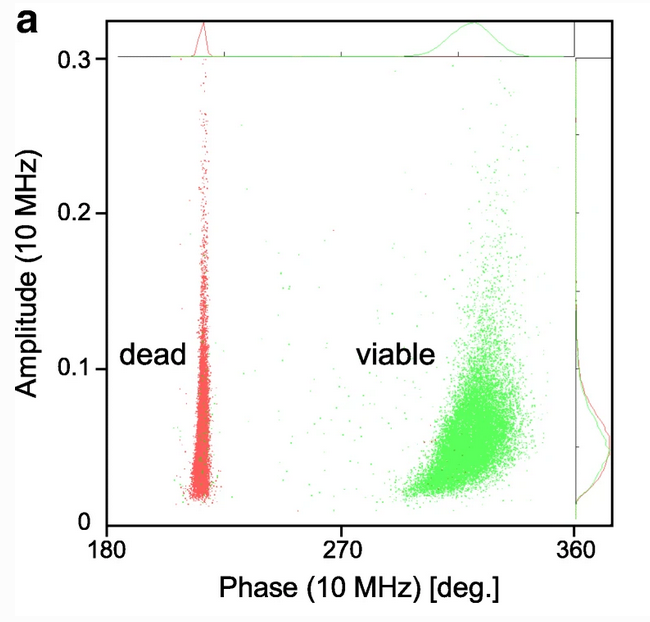
\includegraphics[width=0.6\textwidth]{ScatterGram}
    \caption{Impedance amplitude and phase scattergram used to differentiate between live and dead cells.\citep{Opitz2019}}
    \label{fig:ScatterGram}
\end{figure}

IFC has already proven its usefulness for cell differentiation (stained vs unstained, alive vs dead cells) \cite{Carminati2017,david2012viability, prakash2005cmos,Opitz2019}. The soft cell membrane of animal cells loses their electrical properties upon death, which translates into a decrease of the measured impedance difference at intermediate frequencies. Using such tricks, it is possible to differentiate different cells state or modification to their environment. These techniques are however not generalizable to every microparticles. A case-by-case methodology must be elaborated. For instance, bacteria and yeast generally have rigid cell walls, meaning that they keep their membrane properties upon death. Probing at higher frequency inside the cytoplasm could, however, solve this issue \cite{david2012viability,Opitz2019}. Information on the cell membrane capacitance, used in conjunction with the cell size, can be sufficient to discriminate between different blood leukocytes. Using high frequency measurements can determine if a cell is invaded by parasites by probing the cell’s internal composition \cite{Sun2010}.  IFC can also be used to gain information about the status of the cell culture. For example, there is a phase shift towards lower value of phase when the cell population transitions from the exponential to the stationary growth phase. In yeast culture, the cells begin to grow in the lag phase, before dividing and then maintaining a smaller average cell similar to that of a dead cell \cite{Opitz2019}. \par

The differential impedance spikes observed at the output are used to count the number of particles passing in the channel, as well as determining the particle size, morphology, and composition. A simple detection algorithm would be to fix a rigid threshold for a specific impedance value such that whenever the impedance goes above that threshold, a particle is recognized by the algorithm. The amplitude and size of that pattern can be used to deduce the cell parameters and fluid flow. Other more complex detection methods can be used, such as segmentation, autocorrelation, leveraging the odd symmetry of differential pulses, machine learning , etc. \cite{Carminati2017}. \par

The position of the cell in the channel influences the measured signal due to the non-homogeneous electrical field distribution of coplanar electrodes. A higher particle in the channel will experience weaker electrical field than a low particle, which will result in a lower perceived amplitude \cite{De_Ninno2017,caselli2018novel}. Since the amplitude of the spike is used to infer the cell properties, a significant error is thus observed. three solutions can be used to counter this problematic: (1) Using parallel facing electrodes placed diagonally opposed in the channel, as proposed by \citep{caselli2018novel}. This technique however requires parallel electrodes, which adds complexity to the microfabrication. (2) A The structure of the electrodes themselves can be modified, as shown in \autoref{fig:DeNinno2017}, to create specific signal pattern whose shape can be used to identify the vertical position of the particle in the channel (such shapes are also found to be more robust against noise)  \cite{Carminati2017,De_Ninno2017}. The relative prominence of the shapes obtained, coupled to the transit time of such shape, are parameters that depend on the geometry of the channel and electrodes, such that corrected particles parameters can be retrieved from post-processing calculations. This method, however, reduces the sensibility of the measured pulses since the sensing volume increases when using multiple electrodes \cite{petchakup2017advances}. (3) Centering techniques such as dielectrophoresis, acoustophoresis, inertial focusing and sheath flows can be used in the microfluidics to put the cells exactly where they are needed. This second solution is, however, more complicated and has quite a lot of shortcomings, but at least doesn’t require complex post-processing calculations \cite{De_Ninno2017}. \par
\begin{figure}[h]
    \centering
    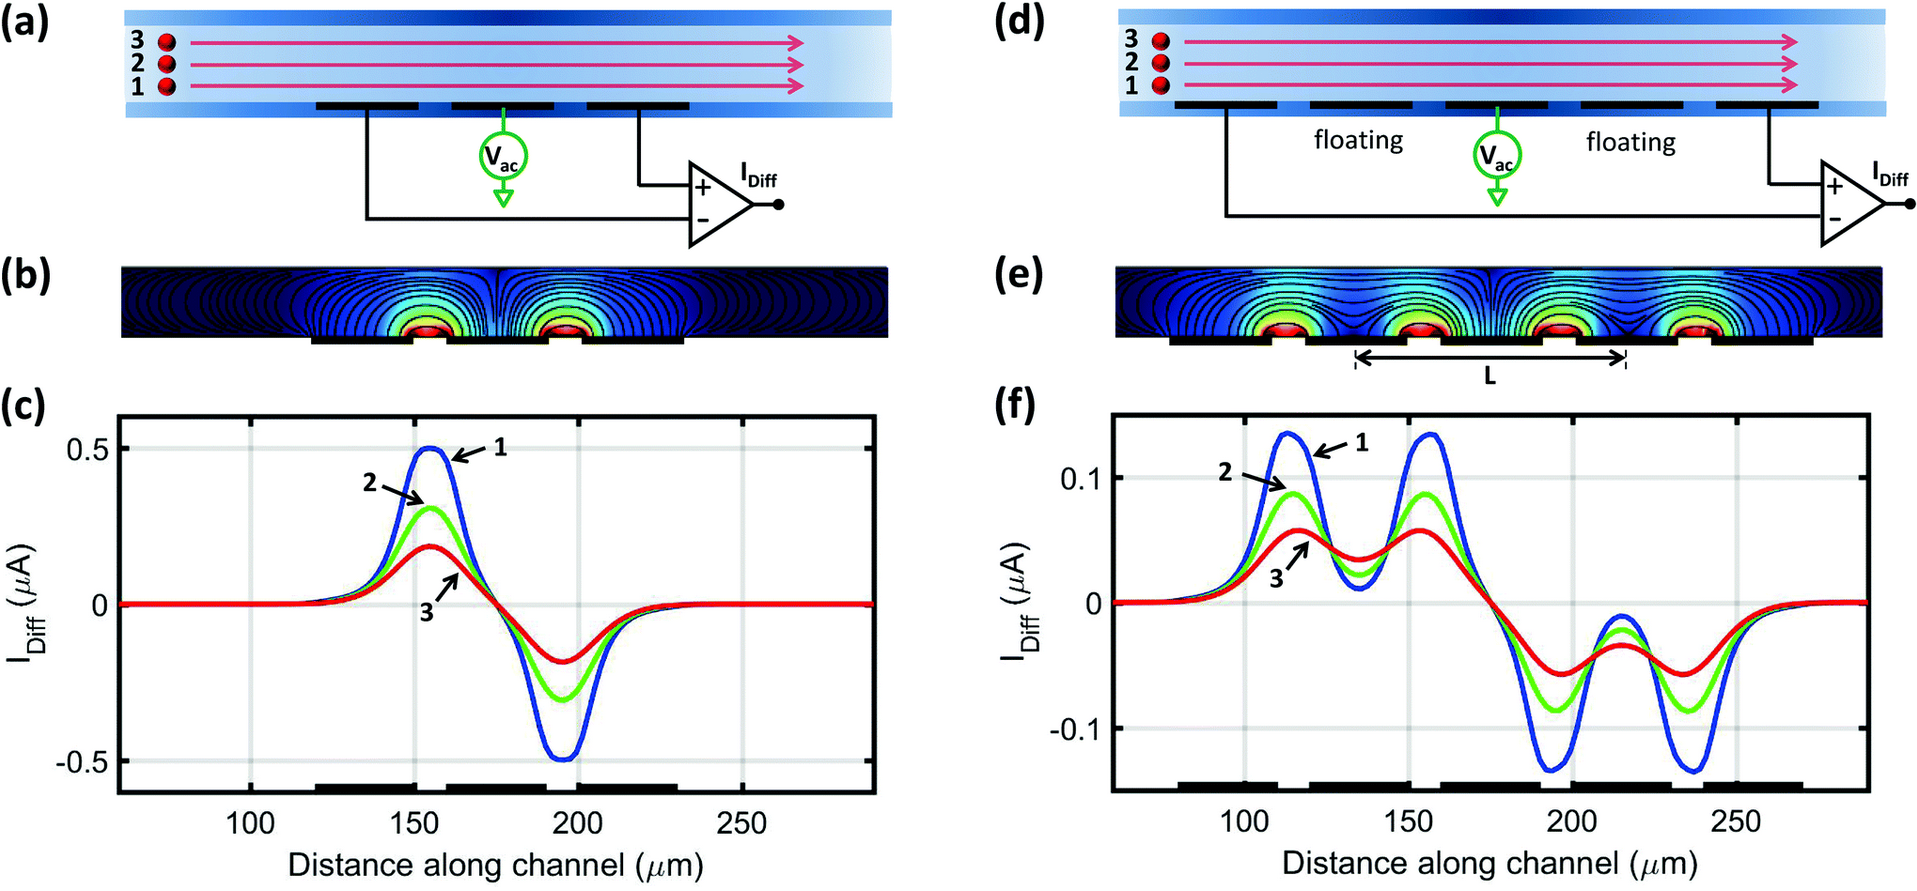
\includegraphics[width=1\textwidth]{images/DeNinno2017.png}
    \caption{A conventional differential 3-coplanar electrodes signal response, compared to the configuration when two floating electrodes are added. Note the difference in signal response in function of the height of the particle in the channel.\citep{De_Ninno2017}}
    \label{fig:DeNinno2017}
\end{figure}

IFC is quite tolerant to multiple medium conductivity and conditions. A conductivity between 2 and 10 mS/cm is generally deemed adequate. The number of cells should however be kept low enough such that the channel does not clog or that multiple particles pass the electrodes at the same time, resulting in a bigger signal output. Simply diluting the sample is an effective action to counter that. Adding a surfactant to the buffer, such as soap, proves itself adequate to prevent chain forming microparticles. A filter might also be used to remove large impurities \cite{Opitz2019}. These fluidics concerns will be discussed in \autoref{chap:Microfluidics}.

\chapter{Electronic modules}
\label{chap:Electronics}
The different electronics modules used for the impedance-sensing system are discussed in this chapter. A theoretical overview is provided to better understand the way the impedance-sensing system functions.
\section{Transimpedance Amplifiers}
\label{sec:TIA}
Transimpedance Amplifiers (TIAs) are current to voltage converters generally implemented using one operational amplifier, as shown in \autoref{fig:TIA_basic} \cite{horowitz1989art}. A current coming from the negative input of the op-amp is amplified and converted to a voltage signal by a feedback resistor $R_f$, while the positive input of the op-amp is connected to the reference. TIAs are negative gains amplifiers similar to inverting amplifiers configuration. For DC applications, their transimpedance follows the equation: 
\begin{equation}
\label{eq:TIA_simple}
G(\omega=0)=\frac{V_{out}}{I_{in}} = -R_f
\end{equation}
Large values of feedback resistors are generally chosen in TIAs since the transimpedance increases linearly with $R_f$, while the output voltage noise, when only considering  the Johnson-Nyquist noise due to the thermal agitation of charge carriers, increase proportionally to its root mean squared value \cite{horowitz1989art}. This leads to an input-refered noise current proportional to the inversed root mean square of $R_f$: 
\begin{equation}
\sqrt{i_{n,in}^2}=\sqrt{\frac{4 k_B T \Delta f}{R_f}}
\end{equation}
However, choosing large values of $R_f$ induce considerable output offset voltage and large output voltage swing \cite{horowitz1989art}. It is thus recommended to use op-amps based on Field-Effect Transistors (FET) that present a low input offset voltage, and op-amps featuring a high gain-bandwidth product when higher excitation frequencies are used \cite{horowitz1989art}. \par
\begin{figure}[h]
    \centering
    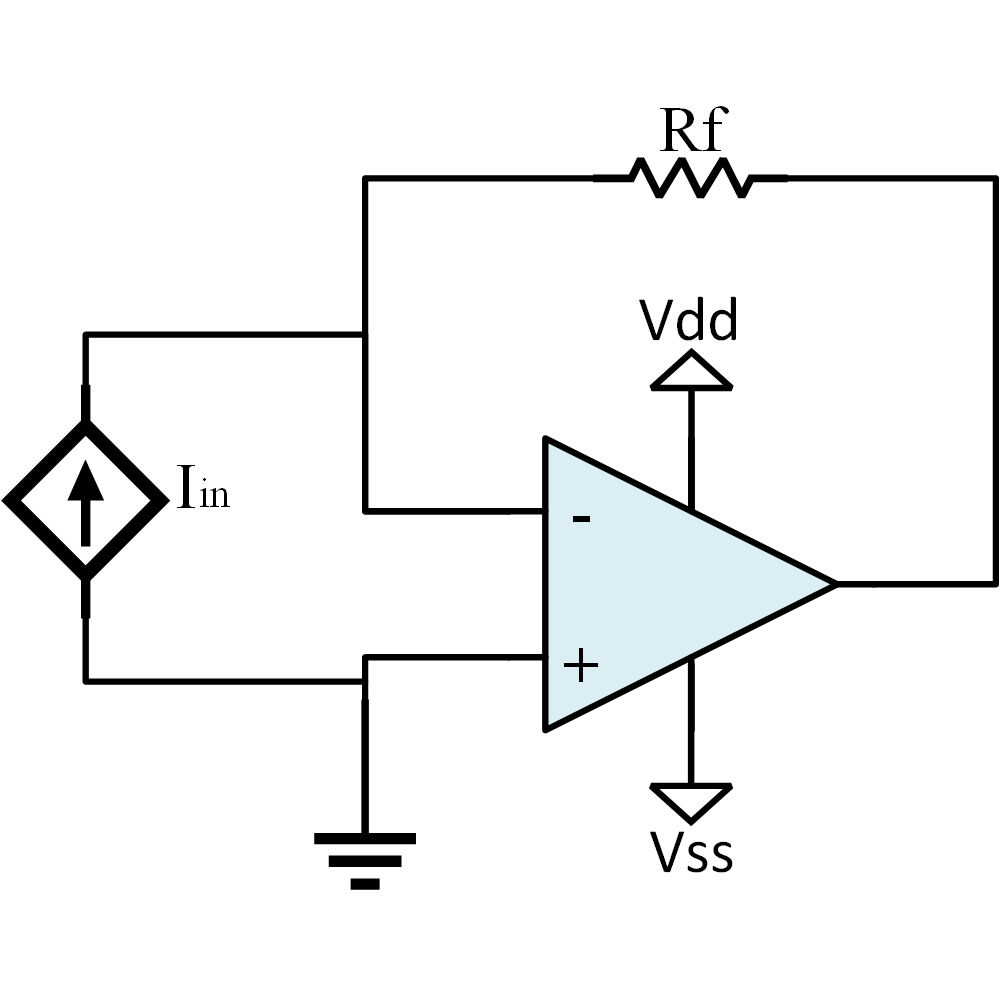
\includegraphics[width=0.5\textwidth]{TIA_basic}
    \caption{A basic discrete TIA made from one op-amp and one resistor.}
    \label{fig:TIA_basic}
\end{figure}
A case must be presented concerning the stability of TIAs. An input capacitance $C_i$, often caused by parasitics or by the sensor itself, introduces a pole in the transfer function which induces oscillation at a specific frequency $f_i$ \cite{horowitz1989art}. This is the case since a negative phase-shift is created by the pole, which, when combined with the $180^{\circ}$ phase inversion of the TIA, can induce a full 360 $^{\circ}$ phase-shift, effectively producing a positive feedback loop. If this positive feedback is obtained for a unity or larger op-amp open-loop gain $A_{OL}$, unrestricted oscillations will be generated \cite{horowitz1989art}. This can be better shown mathematically, where the output voltage for an uncompensated TIA is described the same way as in Equation XXX, but with an added pole:
\begin{equation}
V_{out}=I_{in} \frac{-R_f}{1+\frac{1+ R_f C_i s}{A_{OL}}}
\end{equation}
A feedback capacitor $C_f$ can be introduced in parallel with $R_f$ to compensate for the added pole, as shown in \autoref{fig:TIA_compensated}. This leads to a phase cancellation of the pole, which, for an adequate choice of $C_f$, negates the positive feedback loop. The new transfer function is described here: 
\begin{equation}
\label{eq:TIA_full}
V_{out}=I_{in} \frac{-R_f}{1+\frac{1+ R_f (C_i + C_f) s}{A_{OL} (1+ R_f C_f s)}}
\end{equation}
There is no proper method to calculate the compensation capacitor $C_f$. Using a large capacitor will result in a decreased amplifier bandwidth, while a small capacitor may be unable to prevent oscillations\cite{horowitz1989art}. A sufficient phase margin should be considered to prevent unwanted anomalies, which justifies using an iterative approach. Another shortcoming of this approach is that the feedback capacitor value is oftentimes really small when using large resistor values. This effectively creates a compromise when designing TIAs between capacitor choice, thermal noise, offset voltage, bandwidth, and stability. 
\begin{figure}[h]
    \centering
    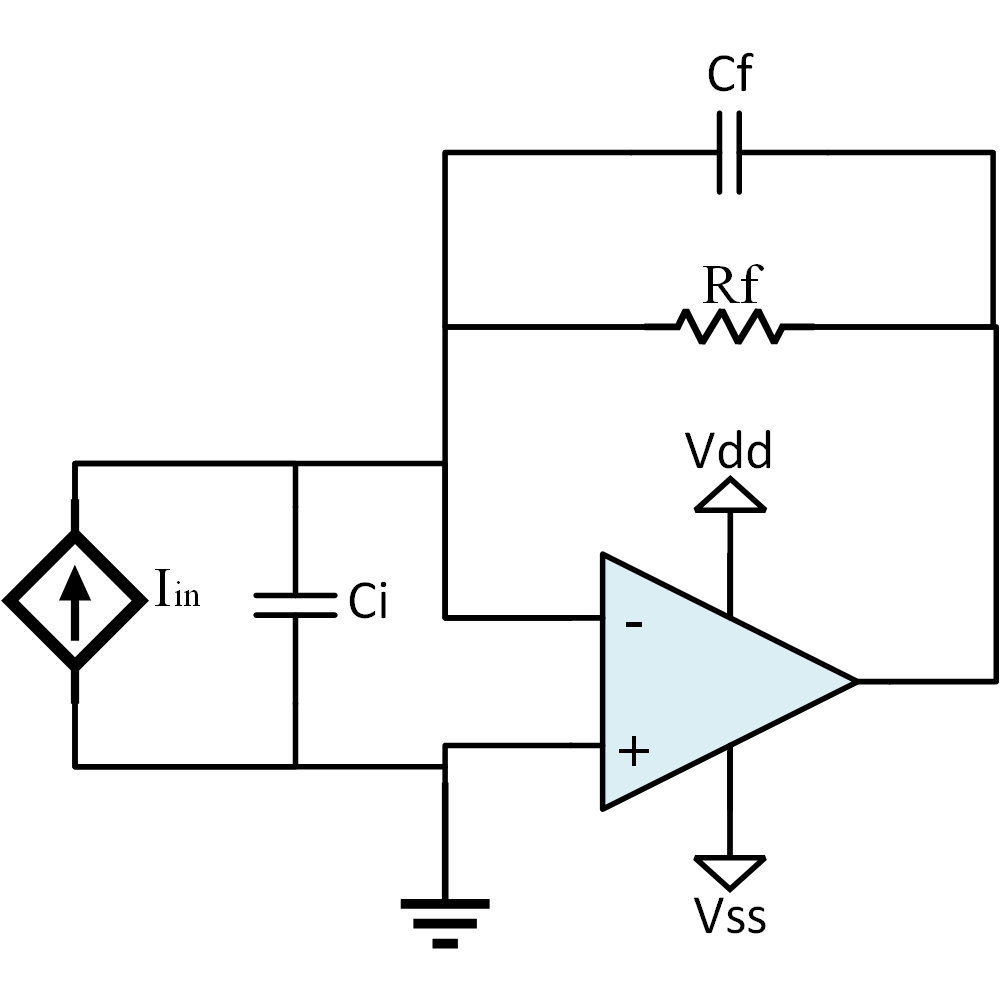
\includegraphics[width=0.5\textwidth]{TIA_compensated}
    \caption{Typical application circuit of a compensated discrete TIA. The pole introduced by the input capacitance $C_i$ is compensated by the feedback capacitor $C_f$}
    \label{fig:TIA_compensated}
\end{figure}
\section{Programmable gain array}
\label{sec:PGA}
Programmable Gain Arrays (PGA) are an electronic scheme to modify on the fly the gain of a system. PGA allow an amplifier to choose from multiple values of gain resistor $R_f$.  This can be achieved with simple relays or multiplexers that can switch when toggled between different resistors \cite{Chabowski2015,horowitz1989art}. The gains are generally controllable by the MCU (see \autoref{sec:MCU}) and the PGA is generally placed in the feeback loop of an amplifier. An exemple of a PGA is provided in \autoref{fig:PGA}.
\begin{figure}[h]
    \centering
    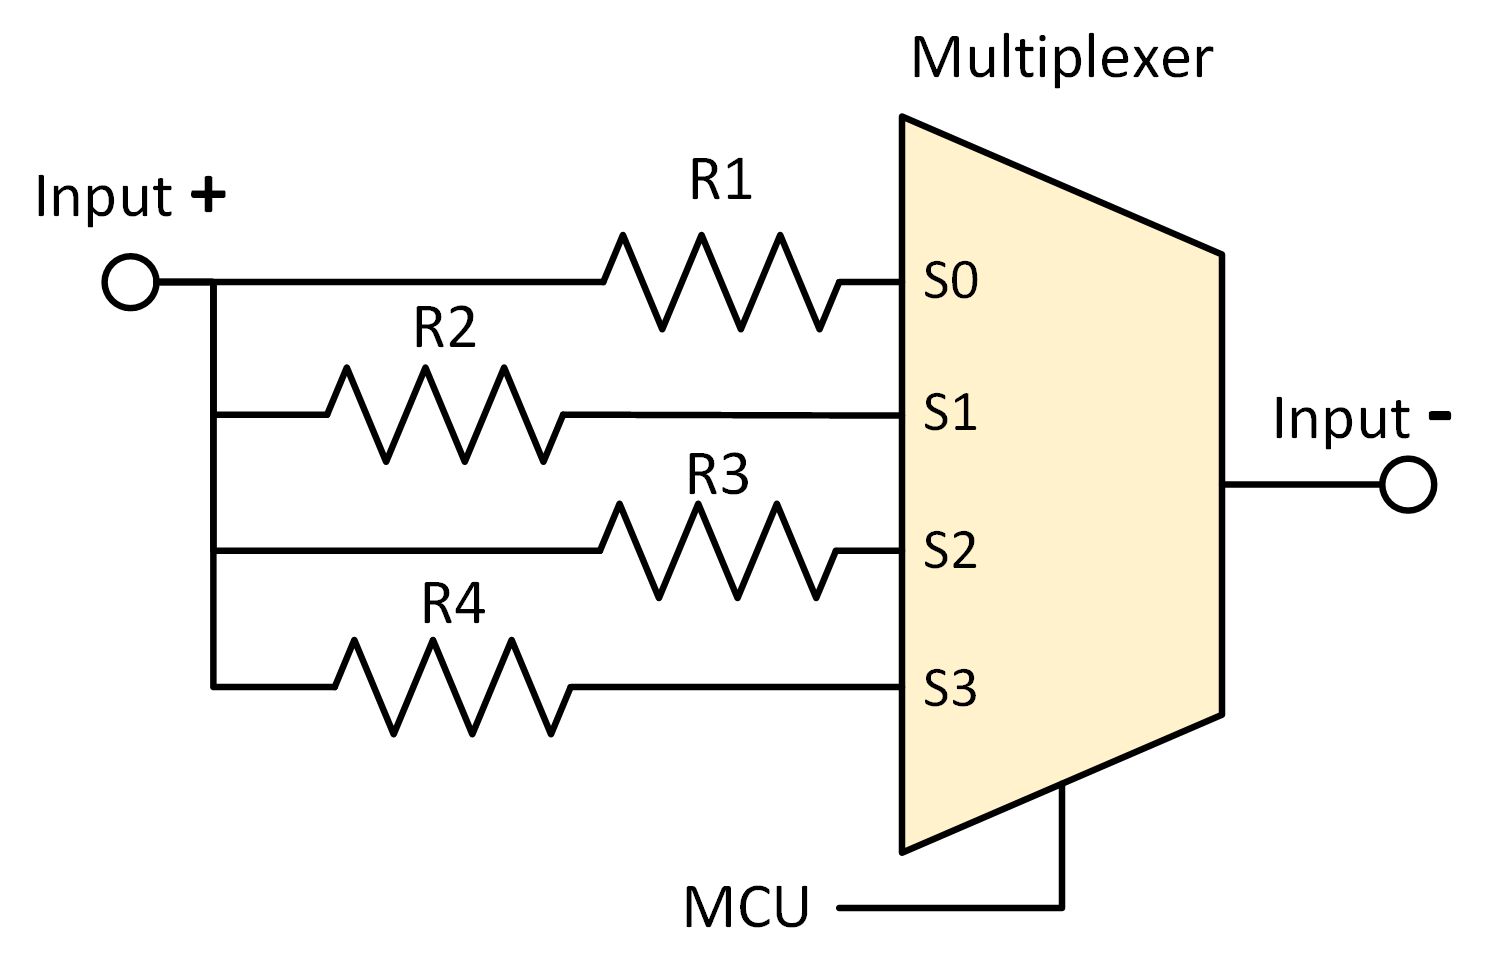
\includegraphics[width=0.7\textwidth]{PGA}
    \caption{Implementation of a PGA using switchable resistors controlled by a multiplexer.}
    \label{fig:PGA}
\end{figure}
\section{Lock-In Amplifiers}
\label{sec:LIA}
Lock-in Amplifiers (LIAs) are amplifiers that extract the amplitude and phase of a signal with a known frequency from a noisy environment, as shown in \autoref{fig:LIA_principle}. They act as narrowband filter to precisely measure the amplitude of a signal hidden by noise \cite{Carminati2017,horowitz1989art}. \par 

\begin{figure}[ht]
    \centering
    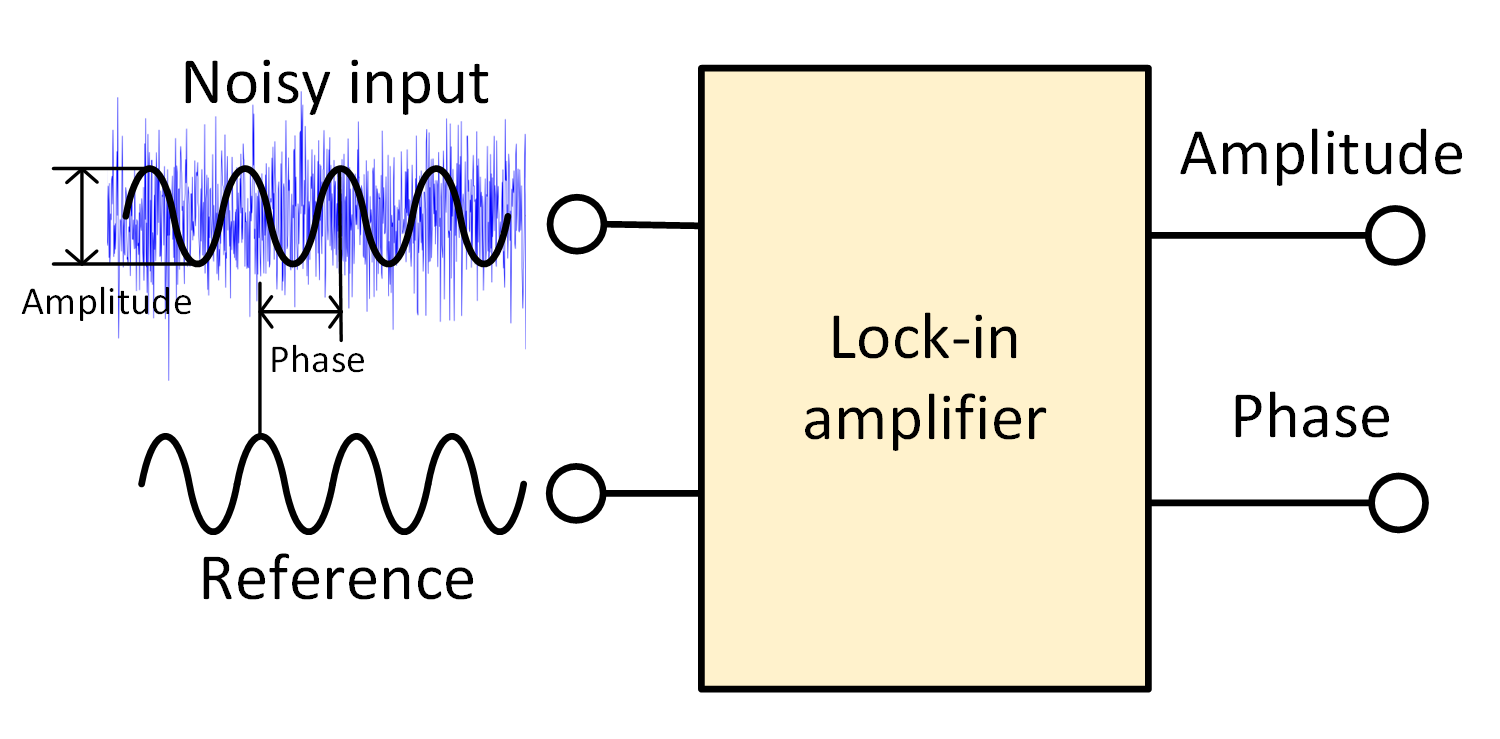
\includegraphics[width=0.7\textwidth]{LIA_principle}
    \caption{Basic principles of a LIA. The amplitude and phase components can be retrieved from a noisy environment.}
    \label{fig:LIA_principle}
\end{figure}
LIA work by transforming the desired AC signal into a DC signal with an amplitude proportional to the output of the measured signal. Some of these amplifiers use analog frequency mixers and other non-linear schemes to obtain the DC amplitude and then use low-pass filter with analog RC filters \cite{horowitz1989art} to isolate the DC signal \cite{Carminati2017}. The frequency-mixing can be achieved by multiplying the input waveform to a reference signal with the same frequency as the input. Mathematically, multiplying two signals together sends the fundamental of that signal to a DC value, as described in \autoref{fig:Mixing} and \autoref{eq:Mixing} :
\begin{equation}
\label{eq:Mixing}
   U_{mix} = U_{in}(f_1) \times U_{ref}(f_2) = \lvert U_{ref} \rvert \lvert U_{in} \rvert \frac{1}{2} (cos(f_1 - f_2) - cos(f_1 + f_2))
\end{equation}
\begin{figure}[ht]
\centering
\begin{subfigure}{0.35\textwidth}
\centering
    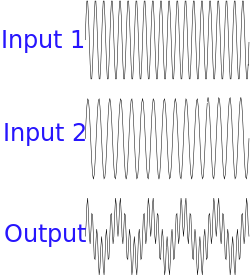
\includegraphics[width=0.8\linewidth]{MixingTime}
    \caption{In time.}
\end{subfigure}
\begin{subfigure}{0.64\textwidth}
\centering
    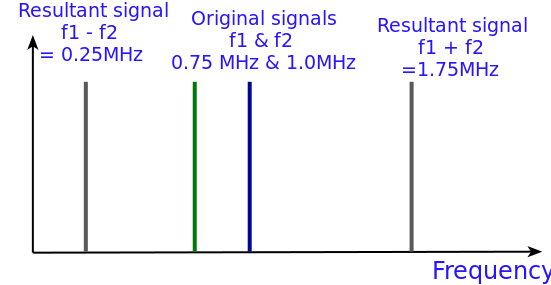
\includegraphics[width=0.9\linewidth]{MixingFreq}
    \caption{In frequency.}
\end{subfigure}
\caption{Mixing two sinewaves of frequency $f_1$ and $f_2$ result in two output signals at frequency $f_1-f_2$ and $f_1 + f_2$ \citep{poole_2020}.}
\label{fig:Mixing}
\end{figure}
For identical frequencies between the reference and input signals and after filtering the high frequency component, only a DC component remains \cite{Carminati2017}, which has an amplitude proportional to half the multiplication of the two signals amplitude: 
\begin{equation}
   \Re(U_{mix-LPF}) = \lvert U_{ref} \rvert \lvert U_{in} \rvert \frac{1}{2} cos(\phi)
\end{equation}
This system can be called a single-phase LIA since a unique in-phase signal has been used for mixing \cite{horowitz1989art}. The phase component $\phi$ in a single-phase LIA can create a significant error if some delay or parasitic capacitances are present in the system and the angle $\phi$ gets further away from 0°. By using a two-phase LIA in quadrature-mode, it is possible to remove the precision loss caused by the unknown phase parameter \cite{horowitz1989art}. Being in quadrature mode means that two reference signals are used, one called the in-phase component at a phase of 0°, and a quadrature component which is phase-shifted by 90°. This creates an in-phase real output $\Re(U_{mix-LPF})$ which depends on the cosine of the angle $\theta$ and a quadrature imaginary output $\Im(U_{mix-LPF})$ which depends on the sine. Using \autoref{eq:Magnitude} and \autoref{eq:Phase}, it is possible to deduce the actual magnitude and phase of the original signals: 
\begin{equation}
   \Im(U_{mix-LPF}) = \lvert U_{ref} \rvert \lvert U_{in} \rvert \frac{1}{2} sin(\phi)
\end{equation}
\begin{equation}
   \lvert U_{mix-LPF} \rvert = \sqrt{\Re(U_{mix-LPF})^2 + \Im(U_{mix-LPF})^2}
\end{equation}
\begin{equation}
   \phi = \atan(\frac{\Im(U_{mix-LPF})}{\Re(U_{mix-LPF})})
\end{equation}
The state-of-the-art LIA is digital since the signal multiplication can be done very efficiently and the phase difference between two signals can be measured precisely using zero crossing algorithms. The mixing scheme of LIA can be implemented efficiently inboard microprocessors or FPGA. However, they are only usable for low to middle frequencies since the signals must first be sampled by the processor’s ADC, which has a limited MCLK frequency \cite{horowitz1989art} This is why analog mixers are used in this project.
\section{Phase-Sensitive Detectors}
\label{sec:PSD}
Phase-Sensitive Detectors (PSD) present an alternative to LIA. PSD uses square signals and an inverter to switch between the original and inverted version of the signal of interest at the frequency of the square reference signal \cite{horowitz1989art}. This switching creates a signal with frequency components at DC and at two times the reference signal. After passing through a low-pass filter, only the DC component proportional to the real and imaginary current of the SUT’s impedance remains. The behavior and implementation of a PSD is shown in figure \autoref{fig:PSD_circuit}. The main advantage of PSDs is that they replace the complex hardware associated with conventional sinewave spectroscopy with much simpler clock-based circuitry \cite{Subhan2019}. For instance, the DAC, wave generator, and linear mixer can all be replaced by a simple clock generator and controlled switches. This leads to a decrease of the system’s power-consumption, which is primordial in portable application \cite{Subhan2019}. \par
\begin{figure}[h]
    \centering
    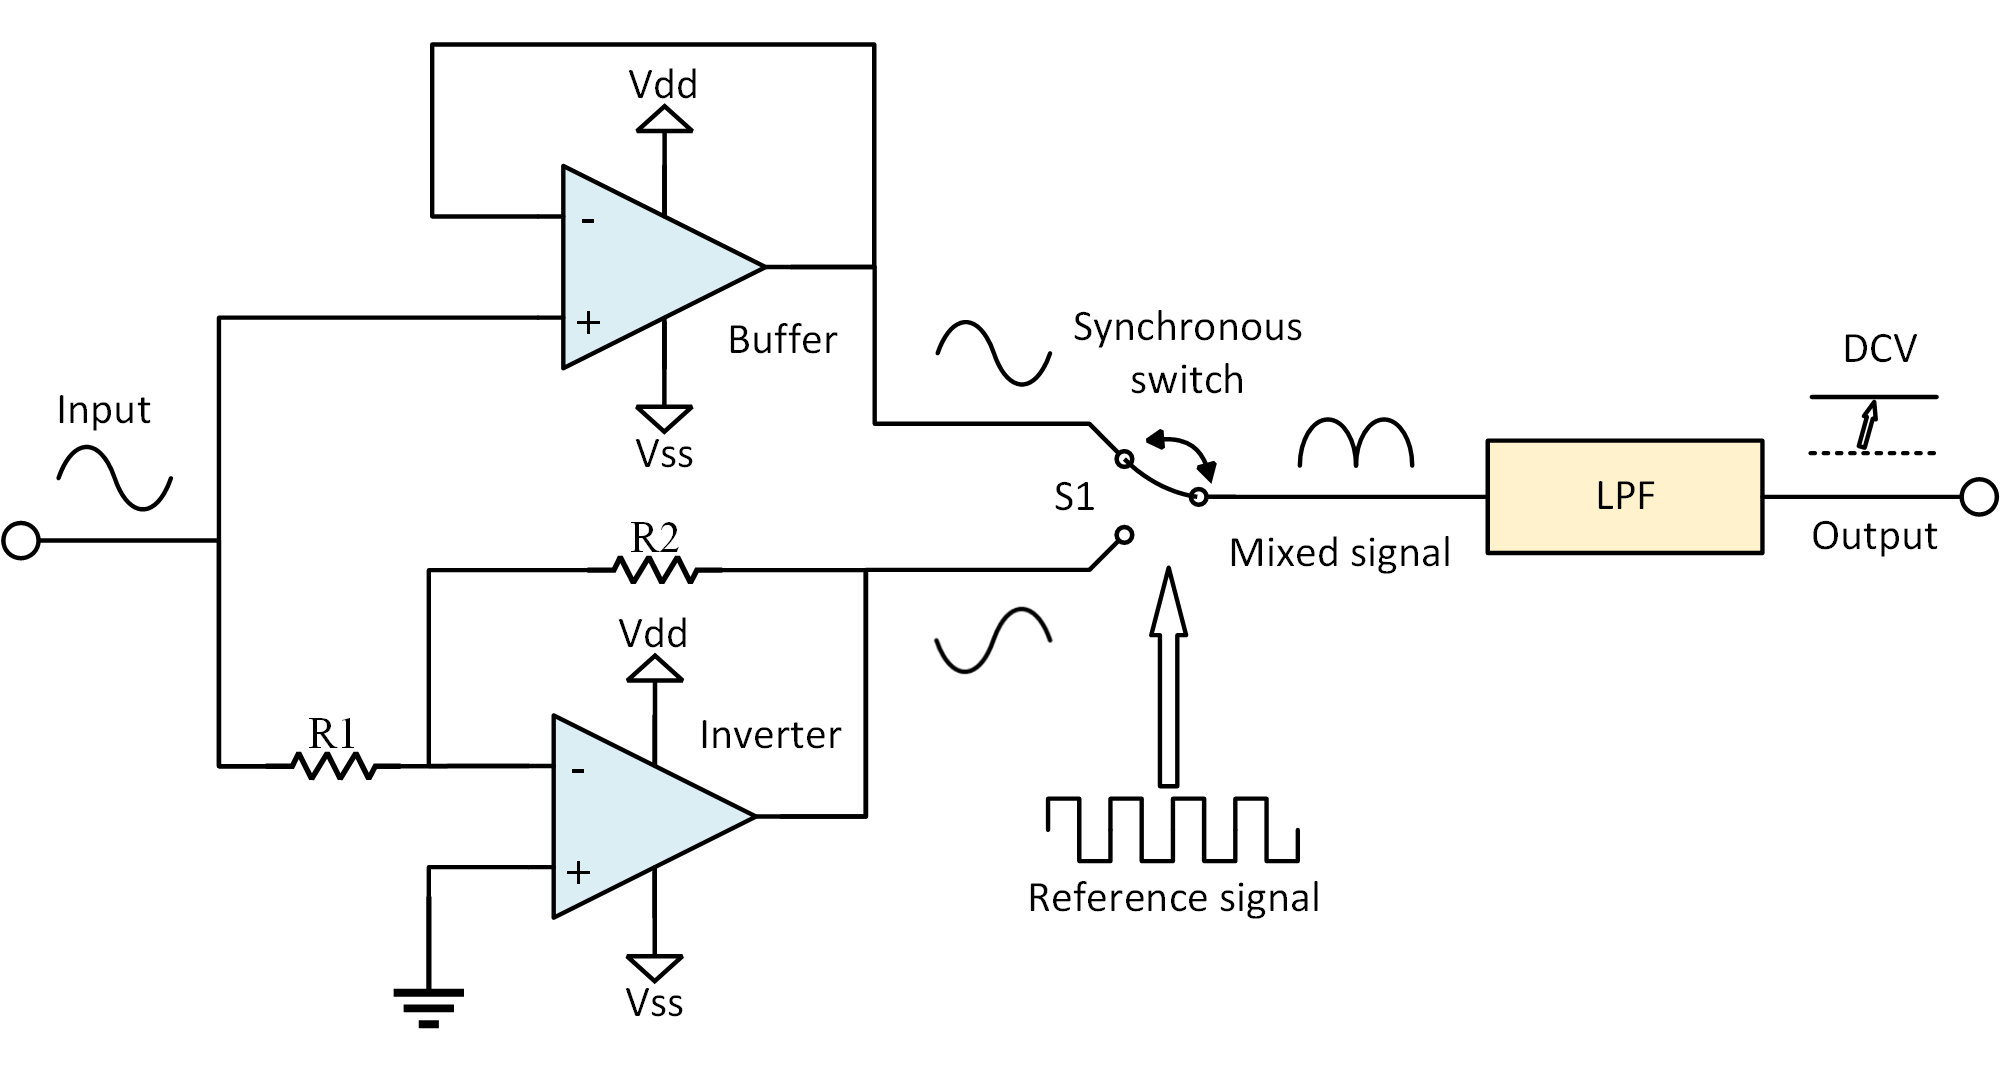
\includegraphics[width=1\textwidth]{PSD_circuit}
    \caption{Behavior and implementation of a PSD circuit.}
    \label{fig:PSD_circuit}
\end{figure}
PSD are, however, less precise compared to LIAs or other systems based on sinewaves. As will be described in \autoref{sec:ImpedancePrinciples}, using square waves introduce a systematic error in the amplitude measurement, which can be mostly corrected in post-processing if multiple frequency points are sampled. This error introduces errors of less than 2\%. Another consideration is the introduction of harmonics in the system, which raises the noise floor of the circuit \cite{Subhan2019}. 
\subsection{Square excitation signals}
\label{sub:SquareSignal}
Square signals are multi-frequency signals. Taking their Fourier transform, it is possible to see that a square wave is composed of a fundamental frequency followed by odd-frequency harmonics with decreasing amplitudes \cite{Subhan2019}. An ideal symmetrical square wave of amplitude 2 with peaks at -1 and 1 \cite{ramaley1969theory} follows this equation:
\begin{equation}
   x(t) = \frac{8}{\pi} (sin(\omega t) + \frac{1}{3} sin(3 \omega t) + \frac{1}{5} sin(5 \omega t) + \frac{1}{7} sin(7 \omega t) + \dots)
\end{equation}
Such a geometrical sum can be better shown as follows \cite{Subhan2019,ramaley1969theory}:
\begin{equation}
\label{eq:Squarewave}
   x(t) = \frac{8}{\pi} \displaystyle\sum_{n=1,3,5,7...} ^{\infty} \frac{(sin(n \omega t)}{n} 
\end{equation}
An important point to note from this equation and from \autoref{fig:SquareWave} is that the amplitude of the fundamental differs from the one of a sinewave of amplitude 2 \cite{ramaley1969theory}. Such a difference $\frac{8}{\pi} \neq 2$ will affect the measurements later on, but can be corrected in post-processing (see \autoref{sec:ImpedancePrinciples}) \cite{Subhan2019}. 
\begin{figure}[h]
    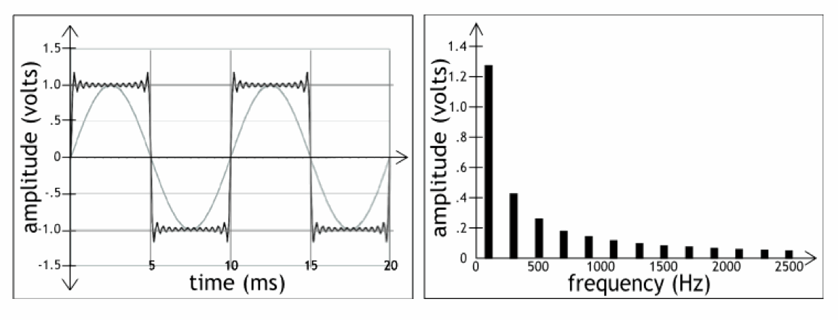
\includegraphics[width=1\textwidth]{SquareWave}
    \caption{Symmetrical practical square-wave of amplitude two described as a function of time and frequency.}
    \label{fig:SquareWave}
\end{figure}
\section{Quadrature generators}
\label{sec:QuadratureGenerator}
In order to use the PSD, two quadrature reference signals are needed. A quadrature generator is an electronical circuit that creates a 90° phase shifted replica of an input signa \cite{Jorgesen2015}. Such a quadrature generator can be created using a comparator and two D-Flip-Flops \cite{horowitz1989art}, as shown in \autoref{fig:QuadratureGenerator}. The comparator creates a square signal that oscillates between $V_{DD}$ and $V_{SS}$, and an inverted version of that signal. Those two signals are sent to the “clock” input of two D-Flip-Flop. The input of the D-Flip-Flops are connected to their own inverted output (effectively transforming the D-Flip-Flop into T-Flip-Flop) \cite{horowitz1989art}. The non-inverted outputs on both Flip-Flop are thus precisely 90° phase shifted from one another, but their frequency is also divided by two compared to the frequency of the signal at the input of the comparator \cite{Jorgesen2015}. \par
\begin{figure}[h]
    \centering
    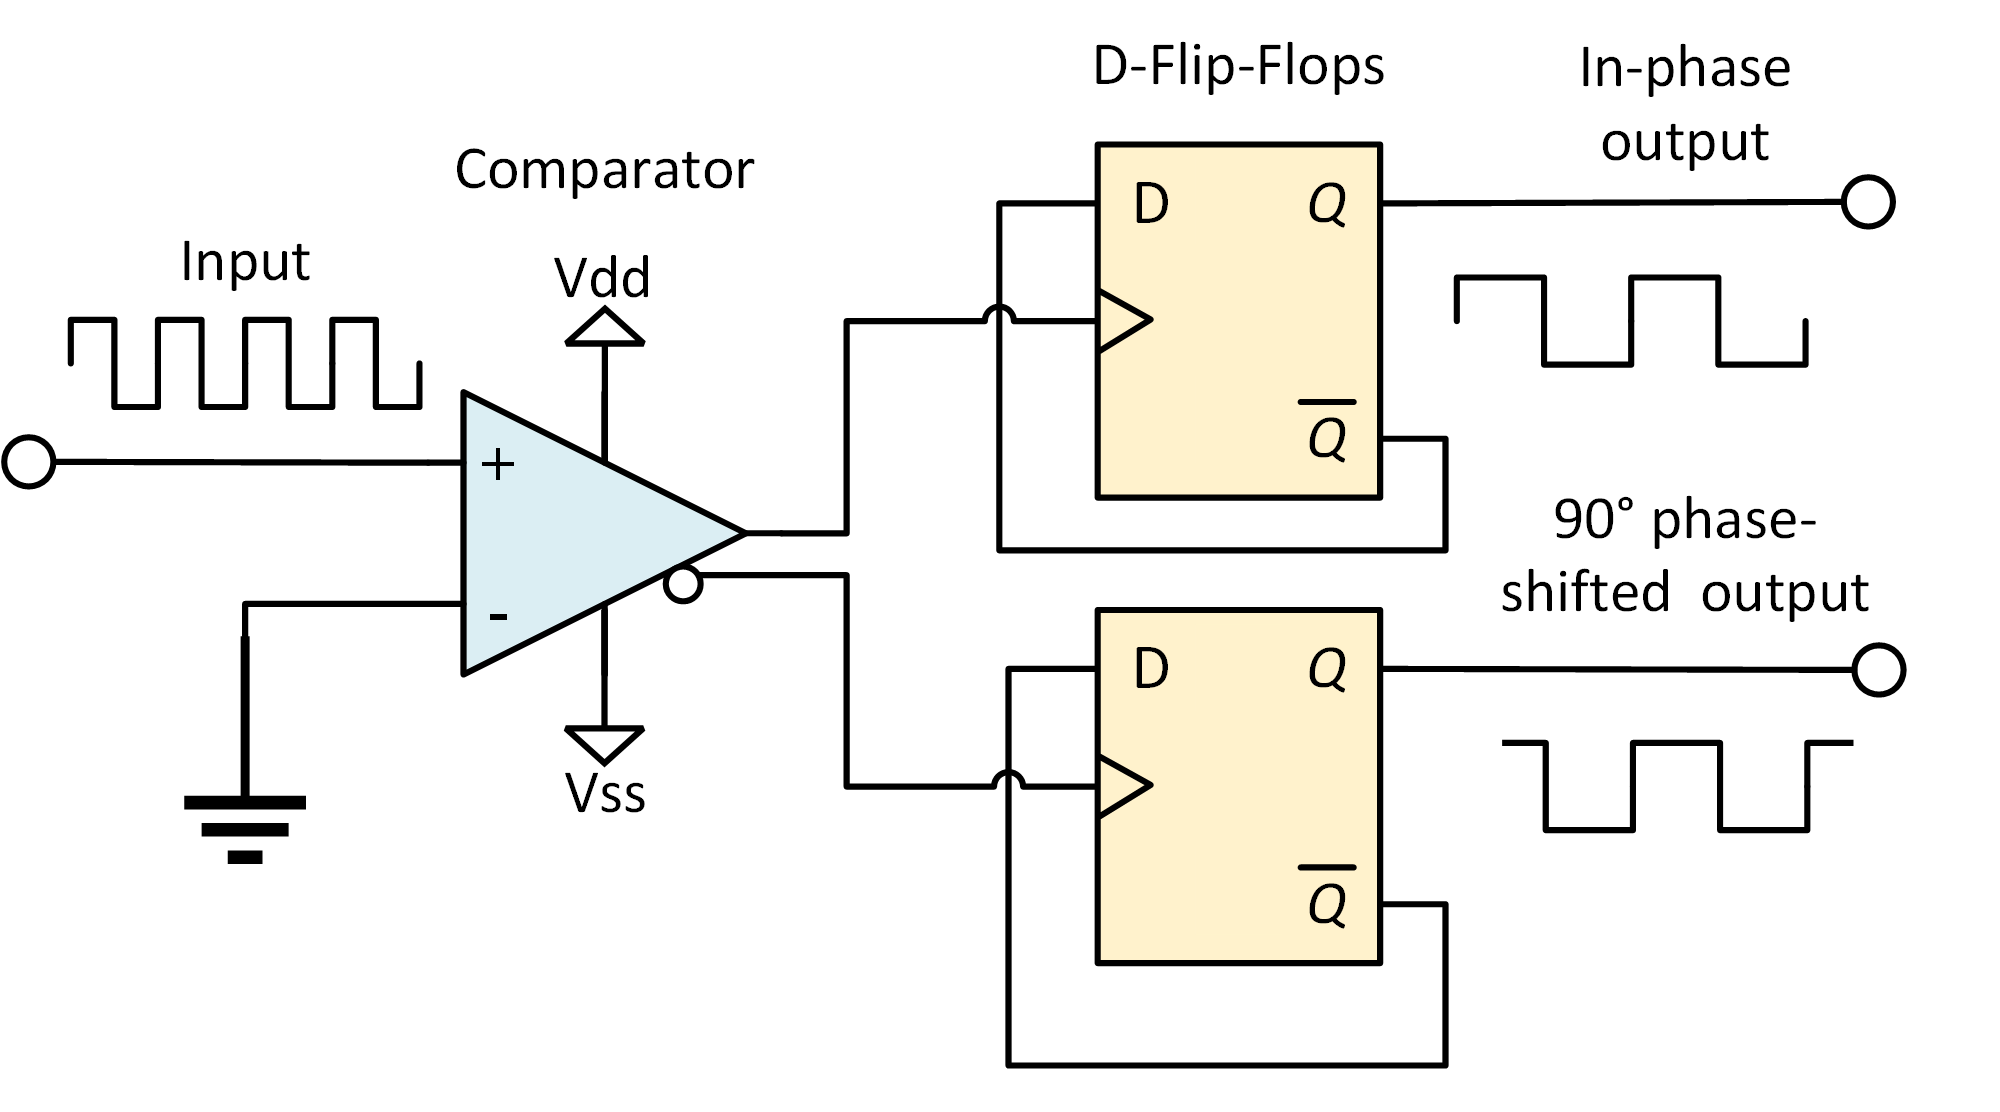
\includegraphics[width=1\textwidth]{QuadratureGenerator}
    \caption{Behavior and implementation of a quadrature generator circuit. Note that the outputs are at half the input frequency.}
    \label{fig:QuadratureGenerator}
\end{figure}
This technique is ultrawideband and relatively simple but can be used only for low-power binary signals. A signal double the output frequency must be provided at the input. They are much affected by duty-cycle errors or phase noise at the input, which are directly seen at the output \cite{Jorgesen2015}.  

\section{Microcontroller Unit}
\label{sec:MCU}
The IFC system uses a MSP430F5529 as a Microcontroller Unit (MCU). The MSP430F5529 is a mixed signal MCU uses for low-power applications. It features a 1.8V to 3.6V power-supply, a 16-bit RISC CPU, a 25MHz maximum Master Clock (MCLK) powered by a digital Frequency-Locked Loop (FLL) powered by a low frequency 32kHz watch crystal, 12-bit ADCs, 63 I/O pins, a 3-channel DMA with an extended memory, 16-bit timers, timers, interrupts, comparators, 5 different Low-Power Modes (LPM). It supports communication with UART, enhanced UART, SPI, I2C, IrDA, USB 2.0, and is programmed/debuggued by JTAG. It dissipates about 6 mW when active and 24 $\mu$W when in LPM. \par

The impedance-sensing system uses:
\begin{itemize}
	\item 6 channels of the 12-bit ADCs to measure: $\Re(V_{PSD-\omega_0})$ and $\Im(V_{PSD-\omega_0})$ of the two electrode responses, the 5V $V_{DD}$ power-supply, and the battery voltage. 
	\item A 32-kHz watch crystal creates a MCLK oscillating at 16MHz with the PLL. 
	\item The I2C module used to program the Si5351 and modify the excitation signal frequency. 
	\item The UART module used with the external IC FT232RL to convert the sampled data to RS232 to be transfered to a nearby computer.
	\item A couple of I/O pins to enable the power-supplies, monitor the status of the system by activating LEDs, modify the gains of the PGA on the fly, modify the phase of the measurement by enabling or disabling the flip-flops of the quadrature generator, and reset the MCU at the press of a button. 
\end{itemize}
\section{Analog-to-Digital Converters}
\label{sec:ADC}
Analog-to-Digital Converter (ADC) are electronic devices that can convert analog voltage signals to digital values, as shown in \autoref{fig:Conversion_AD_DA}. They imply a resolution $R_{ADC}$ and a dynamic range that limit the final precision of the instrument \cite{horowitz1989art}. The ADC converts analog continuous values into digitized ones that follow quantized steps such as those illustrated in \autoref{fig:ADC_voltage_resolution}. The resolution  $R_{ADC}$ of the ADC thus depends on the Effective Number Of Bits ($ENOB$)\cite{leHuy2004circuits} of the system, which is a practical measure of its resolution that takes into consideration the system’s noise floor and the Full Scale Voltage Range $E_{FSR}$ of the power-supplies $V_{DD}$ and $V_{SS}$ (or $V_{RefHi}$ and $V_{RefLo}$, respectively) of the ADC:
\begin{equation}
   R_{ADC} = E_{FSR} (\frac{1}{2})^{ENOB}
\end{equation}
\begin{equation}
   E_{FSR} = (V_{DD}-V_{SS})
\end{equation}
\begin{figure}[h]
    \centering
    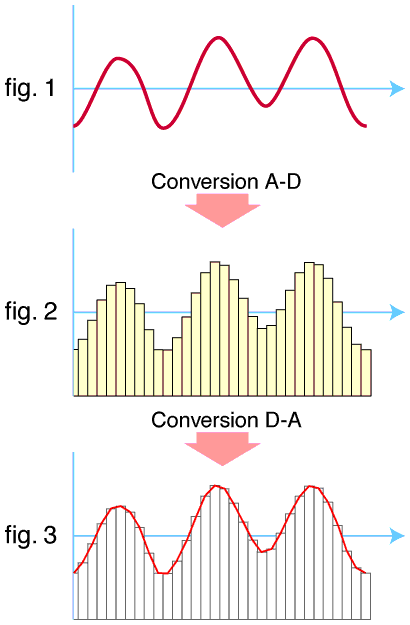
\includegraphics[width=0.4\textwidth]{Conversion_AD_DA}
    \caption{Conversion from the analog (A) domain to the digital (D) domain, followed by a reconstruction in the analog domain.}
    \label{fig:Conversion_AD_DA}
\end{figure}
The $ENOB$ is always slightly lower than the ideal binary dynamic range of the ADC expressed by its number of bits. For a hypothetical 10-bit ADC with an $ENOB$ of 9.5 linked to a unipolar power-supply of 3.3 V, the minimum voltage step would be 4.56 mV. \par
\begin{figure}[h]
    \centering
    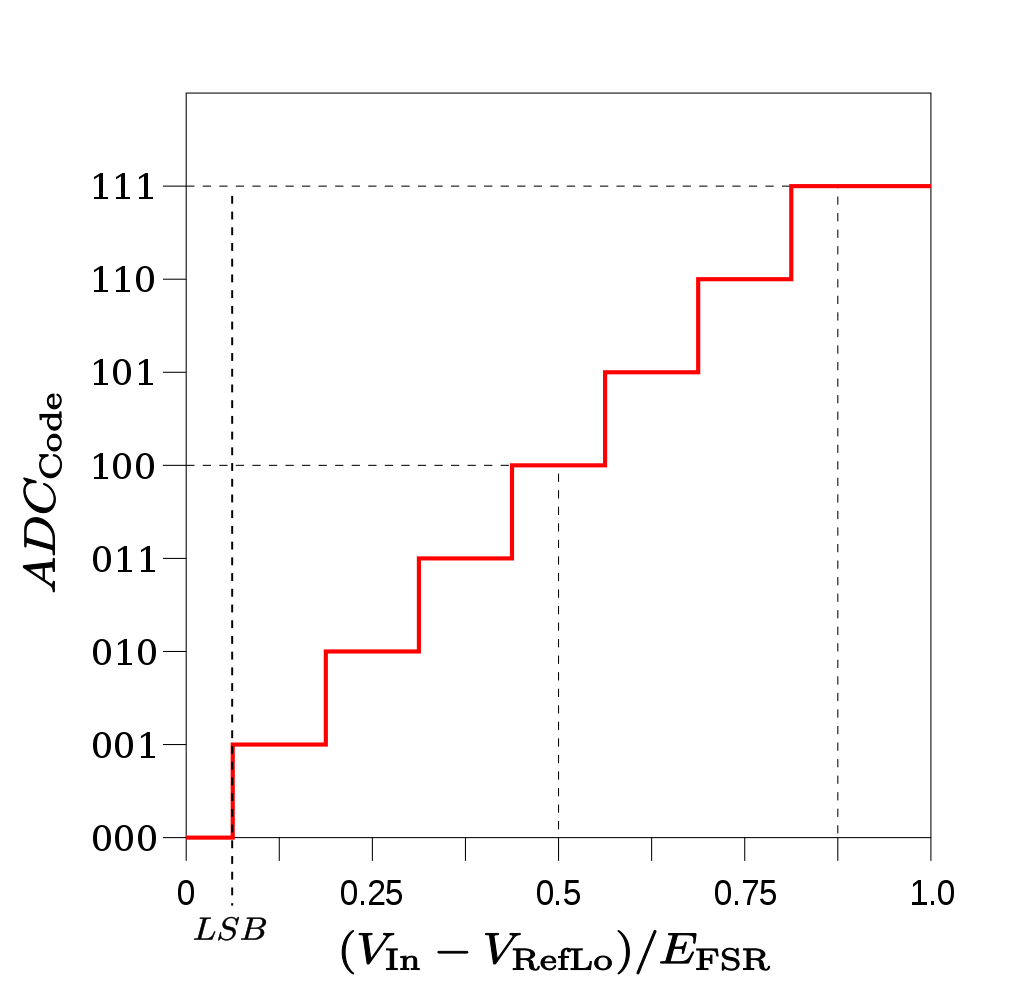
\includegraphics[width=0.6\textwidth]{ADC_voltage_resolution}
    \caption{Resolution increments of a 3-bits ADC.}
    \label{fig:ADC_voltage_resolution}
\end{figure}
\section{Power-supplies}
\label{sec:Power-Supplies}
So that the electronics may work as intended, power-supplies are required. Constant DC voltages with a high current-output must be generated to power the components of the impedance-sensing system. \par

The DC value of these power-supplies depend on the requirements of the chips present in the PCB. For this system, power-supplies of 5V, 3.3V, 2.5V, 1.8V, and 1.65V must be created. The general scheme devised for the power-supplies is that a low-voltage battery of 2.5V would be connected to the PCB. This voltage being lower than some of the power-supplies, a Boost step-up converter is required to create a 5V voltage. The other supplies would be stepped-down from this 5V using linear regulators. The 1.8V supply is used to power the MCU (see \autoref{sec:MCU}) of the system. The MCU needs to be active whenever the system is powered on since it enables the other power-supplies. The whole power-management scheme is shown in \autoref{fig:PowerManagement} \par
\begin{figure}[h]
    \centering
    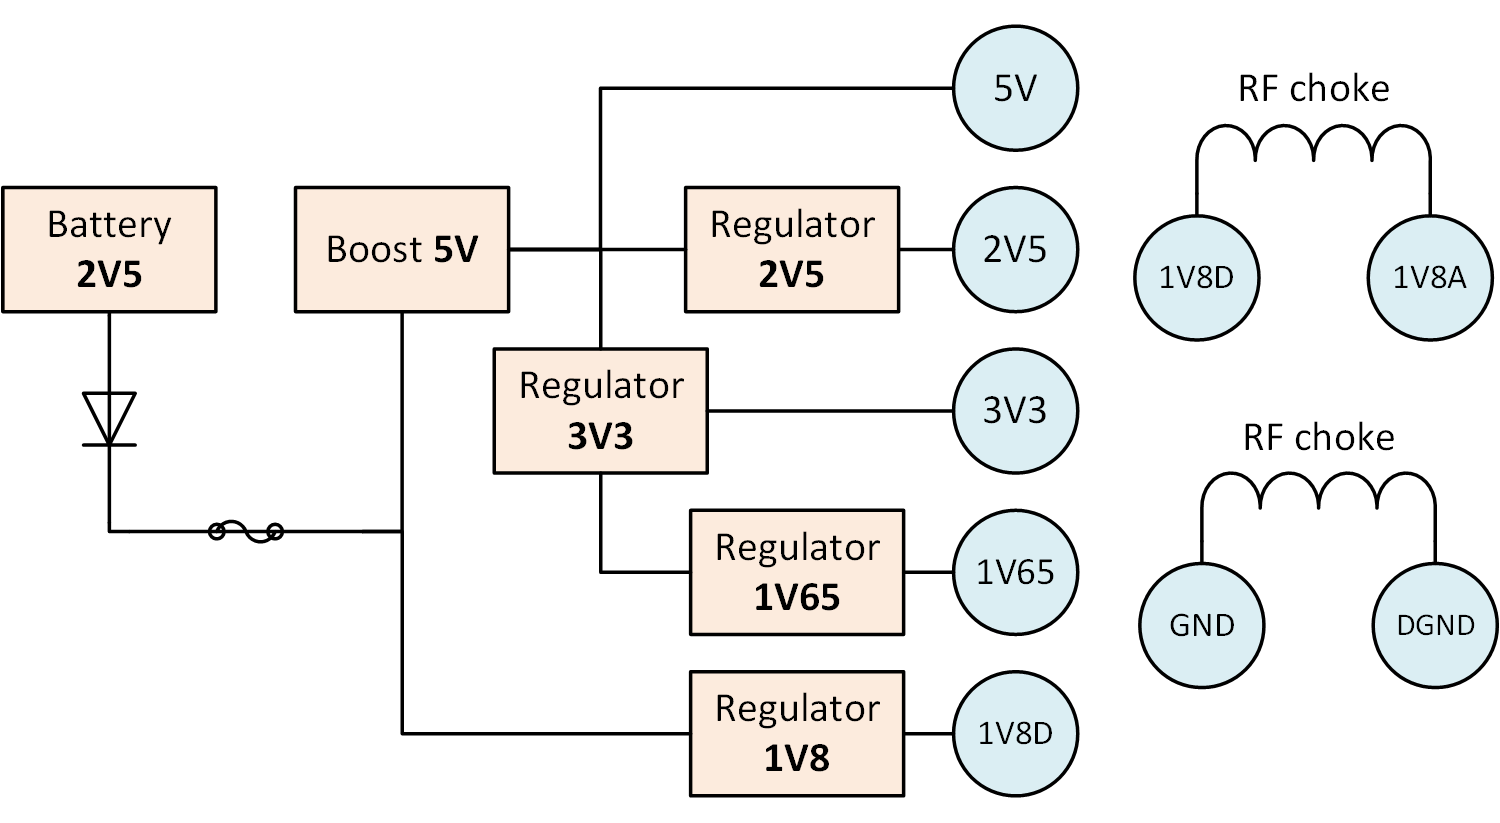
\includegraphics[width=0.9\textwidth]{PowerManagement}
    \caption{Power-management scheme of the impedance-sensing system.}
    \label{fig:PowerManagement}
\end{figure}

Boost converters are adequates supplies for high-power applications since their efficiency is high, upward of 70\%. They do, however, introduce ripples in the system, which increases the noise level at the switching frequency. Adequate filtering is necessary at the converter's output to assure a reference voltage as clean as possible.

Linear regulators are used for the other power-supplies since they demand less power. These types of regulators are precise and linear to the output current, but are not efficient since the regulation voltage (i.e. the subtracted voltage from the input magnitude) is simply wasted as heat and dissipated in the chip. \par

Reference voltages can also be created using a voltage divider and a buffer. Those references, however, cannot provide much power to the load since they are limited by the current output of the buffer. \par

Digital circuitry creates lots of high frequency noise when switching between their binary voltages (0s and 1s), which can introduce high-frequency switching noise in the voltage reference. In order to not contaminate the reference voltages, different planes sharing the same voltages are used. Inductor chokes can be used to reduce the noise shared between reference planes of identical voltages, by linking their DC voltage but blocking the high-frequency components.   \par

\chapter{Practical IFC System}
The practical impedance-sensing system will be described in this chapter, based on the theoretical concepts explained previously in \autoref{chap:Electronics} and \autoref{chap:ImpedimetricSensors}. Practical examples will also be considered to get a sense of the methodology and mathematics. Finally, the PCB will be displayed, as well as the protocol to adequately sample impedance values using the device.
\section{Impedance-sensing system principles}
\label{sec:ImpedancePrinciples}
The bloc-diagram of the impedance-sensing device constructed for IFC application in this memoir is shown in \autoref{fig:BlocDiagramElectronics}. From a bird's eyes view, it works by sending a programmable signal voltage to the SUT, and then measuring it's current response. It uses square waveform as input instead of the conventional sinewave to reduce the power consumption, as explained in \autoref{sec:PSD}. Thus, a square waveform with frequency ranging from 200kHz to 200MHz is created by the clock-component Si5351 \cite{si5351datasheet}. This square waveform is sent to a quadrature generator (see \autoref{sec:QuadratureGenerator}) to create two 90-degree phase-shifted square waveforms at half the clock-component signal frequency. The in-phase waveform is attenuated and sent to the two diffential electrode pairs of the microfluidics system. Their two current responses are amplified and converted to voltage signals by TIAs \cite{horowitz1989art} (see \autoref{sec:TIA}), then mixed by the two PSDs (see \autoref{sec:PSD}). This yields four output signals that can finally be sampled by the ADCs: the real and imaginary current responses of two electrode pairs. The impedance magnitude and phase can be retrieved numerically in post-processing from the real and imaginary impedance components, after correcting the dataset with a square-to-sine algorithm. \par
\begin{figure}[h]
    \centering
    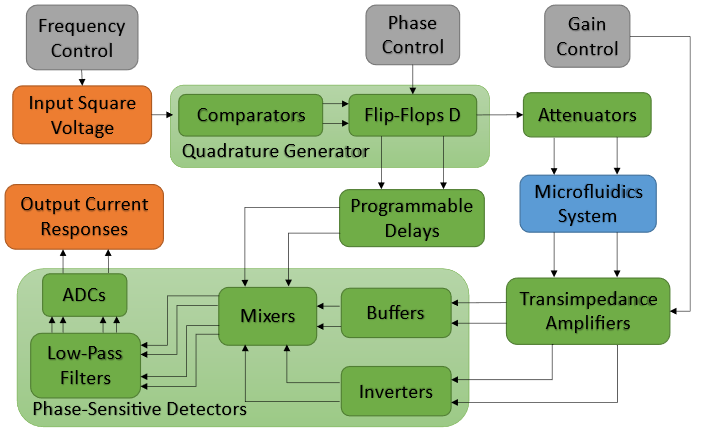
\includegraphics[width=1\textwidth]{BlocDiagramElectronics}
    \caption{Bloc-diagram of the impedance-sensing device constructed in this study.}
    \label{fig:BlocDiagramElectronics}
\end{figure}

Let's describe the methodology in detail from the beginning. \par

The square wave input voltage $V_{in}$ sent to the electrodes is defined in time by \autoref{eq:Squarewave}, as described in \autoref{sub:SquareSignal}. It has a known initial magnitude $V_0$ at the output of the comparator, and is attenuated by a factor $A$ to be at a low enough value of about $~100mV$ for linear impedance measurements that won't harm the cells:
\begin{equation}
   V_{in}(t) = \frac{4}{\pi} \frac{V_0}{A} \displaystyle\sum_{n=1,3,5,7...} ^{\infty} \frac{\sin(n \omega_0 t)}{n}
\end{equation}

This input voltage produces current responses from the two electrode pairs, which follow Ohm's law for complex impedances. This current response being difficult to interact with, two TIAs are used to convert them to voltage signal. Considering the simplified \autoref{eq:TIA_simple} for the transimpedance without $C_f$ and $C_i$, the following equation is obtained:
\begin{equation}
\label{eq:V_TIA}
   V_{TIA}(t) = -\frac{4}{\pi} \frac{V_0}{A} R_f \displaystyle\sum_{n=1,3,5,7...} ^{\infty} \frac{\sin(n \omega_0 t)}{n\lvert Z \rvert (n \omega_0 t + \theta)}
\end{equation}
Where $\lvert Z \rvert (n \omega_0 t + \theta)$ is the impedance magnitude and phase of the SUT at the harmonic frequency $n \omega_0$.  \par

The TIAs current outputs being at high frequency, they cannot be directly sampled by a microcontroller (as already described in \autoref{sec:LIA}). A mixing and filtering stage implemented from a PSD is thus used, which creates DC values proportional to the real and imaginary parts of the current responses (see \autoref{sec:PSD}). These DC values can easily be sampled by ADCs, and follow the equation: \par
\begin{equation}
\label{eq:RealPSD}
   \Re(V_{PSD-\omega_0}) = \frac{1}{2} \frac{6}{\pi^2} \frac{V_0 R_f}{A} \displaystyle\sum_{n=1,3,5,7...} ^{\infty} \frac{\cos(\theta(n \omega_0))}{n^2\lvert Z \rvert (n \omega_0)}
\end{equation}
\begin{equation}
\label{eq:ImPSD}
   \Im(V_{PSD-\omega_0}) = \frac{1}{2} \frac{6}{\pi^2} \frac{V_0 R_f}{A} \displaystyle\sum_{n=1,3,5,7...} ^{\infty} \frac{\sin(\theta(n \omega_0))}{n^2\lvert Z \rvert (n \omega_0)}
\end{equation}
It should be noted that the amplitudes of the reference voltage signal of the PSDs don't influence the previous equations since they are used only to operate the switches. \par 

The real and imaginary outputs of the two PSDs are sampled by four ADCs which have a resolution limit $R_{ADC}$ theoretically fixed by their number of bits, but practically limited by the $ENOB$ (see \autoref{sec:ADC}). This means that a low enough voltage response from the PSDs measured at the ADCs will be undistinguishable from the noise floor. \par

Considering the inverse proportionality of $\lvert Z \rvert$ in \autoref{eq:RealPSD} and \autoref{eq:ImPSD}, the SNR will decrease subtantially as the SUT's impedance increases. To solve this issue, a PGA is added to the system to modify the gain at will (see \autoref{sec:PGA}). This leads to a higher voltage signal at the ADC, which increases the SNR in return. The gain resistor of the PGA should thus always be chosen to maximize the voltage signal, without saturating the ADCs or the op-amps. Indeed, the ADCs and op-amps only operate for voltages in between the power-supplies $V_{DD}$ and $V_{SS}$ (see \autoref{sec:Power-Supplies}). \par

 Now, as can be seen from \autoref{eq:RealPSD} and \autoref{eq:ImPSD}, it isn't trivial to recover the impedance magnitude and phase since harmonics of the square excitation signal are present at every odd frequency of the fundamental \cite{Subhan2019}. Square-waves being used in the mixer instead of sinewaves introduces a systematic error in the impedance measurement. These harmonics are multiplied together by the mixer, which pushes them to DC along with the desired fundamental frequency. Mathematically, this situation adds a geometric sum factor error on the value of impedance measured. This error can be corrected by subtracting the impedance values measured at the harmonics frequencies, as shown in \autoref{fig:SubhanSquare2Sine}. It is thus necessary to measure the entire impedance spectrum before computing the adjusted impedances. \par
\begin{figure}[h]
    \centering
    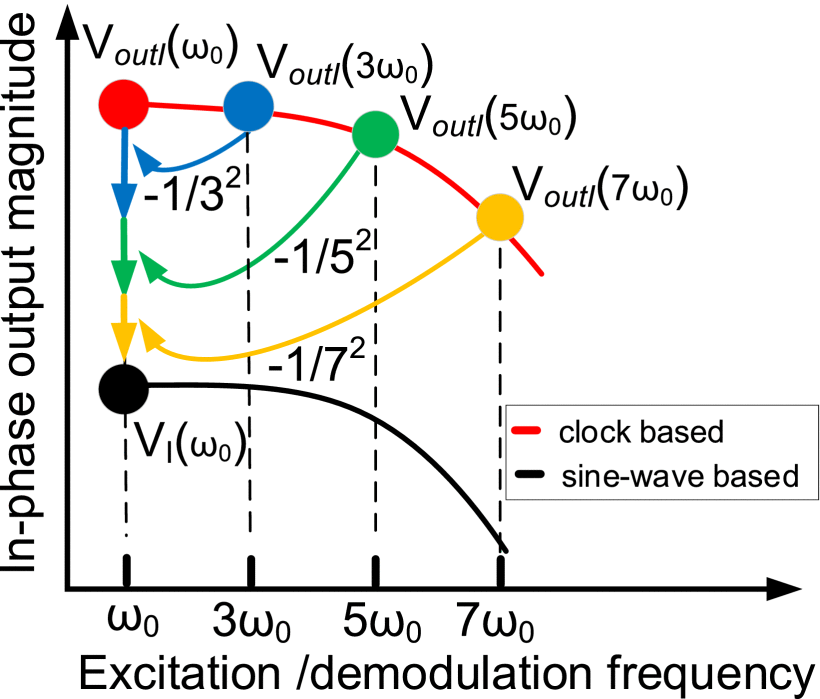
\includegraphics[width=0.7\textwidth]{SubhanSquare2Sine}
    \caption{Illustrated principles of the error-cancellation method proposed by \citep{Subhan2019}.}
    \label{fig:SubhanSquare2Sine}
\end{figure}

This algorithm to convert from a square wave spectroscopy to a sinewave spectroscopy is taken almost directly from \citep{Subhan2019} and modified to fit the system used in this study. The values of square impedances at the harmonics can be subtracted or added to the fundamental impedance following a certain set of rules described in \citep{Subhan2019}. Following these rules, it is possible to retrieve the impedance spectroscopy real and imaginary components devoid of the systematic error $V_{sine-\omega_0}$. This process is described here :  
\begin{align}
\label{eq:correctionReal}
   \Re(V_{sine-\omega_0}) &= \displaystyle\sum_{n=1,3,5,7...} ^{\infty} \frac{\cos(\theta(n \omega_0))}{n^2\lvert Z \rvert (n \omega_0)} - \displaystyle\sum_{n=3,5,7...} ^{\infty} \frac{\cos(\theta(n \omega_0))}{n^2\lvert Z \rvert (n \omega_0)}\nonumber\\
   \Re(V_{sine-\omega_0}) &= \frac{\cos(\theta(\omega_0))}{\lvert Z \rvert (\omega_0)} + E
\end{align}
Where $E$ is the residual error after correction. The same process can be repeated for the quadrature component:
\begin{equation}
   \Im(V_{sine-\omega_0}) = \frac{\sin(\theta(\omega_0))}{\lvert Z \rvert (\omega_0)} + E
\end{equation}
The corrected impedance magnitude and phase can then be reconstructed based on \autoref{eq:Magnitude} and \autoref{eq:Phase}.
\begin{equation}
    \label{eq:CorrectedMagnitude}
   \lvert Z(\omega_0) \rvert = \frac{1}{2} \frac{6}{\pi^2} \frac{V_0}{A} R_f \frac{1}{\sqrt{(\Re(V_{sine-\omega_0}))^2+(\Im(V_{sine-\omega_0}))^2)}}
\end{equation}
\begin{equation}
\label{eq:CorrectedPhase}
   \theta(\omega_0) = -\atan(\frac{\Im(V_{sine-\omega_0})}{\Re(V_{sine-\omega_0})})
\end{equation}
\section{Example measurement}
\subsection{Resistive example}
The signals at every electronics modules' output are shown in \autoref{fig:IFCPracticalExample} for the case of a 1k$\Omega$ resistor SUT: (1) A 3.3V square signal at a frequency between 10kHz and 200MHz exits the Clock generator Si5351 \cite{si5351datasheet}. (2) This signal is sent to a comparator, which saturates it to $V_{DD}$ at 5V. The comparator also outputs an inverted signal. (3) The outputs of the comparator are sent to the D-flip-flops, which produce two signals at half the input's frequency and that are 90 $^\circ$ phase-shifted from each another. The flip-flops are digital circuit, meaning that they work only as 1s and 0s. The positive output of the flip-flops are thus not exactly at $V_{DD}$; there is a voltage loss that appears at the output of the flip-flops, rendering the magnitude to 4.3V. (4) The in-phase signal is sent to an attenuator, which reduces the amplitude of the signal from a factor $17$ between 2.374V and 2.626V. (5) This signal is sent to the 1k$\Omega$ resistor (SUT) which produces a current response. This current response is converted back to a voltage by a TIA with a feedback resistor value of 10 000$\Omega$, putting the signal at the output of the TIA to be between 1.235V and 3.765V. (6) A buffer and an inverter produce inverted inputs, which are fed to the mixers. (7) The in-phase output of the mixer gets to a higher quasi-DC voltage of 3.765V, with small spikes to 1.235V caused by the delays in the electronics at the switching times. (8) The quadrature output of the mixer switches at a double frequency value than the input, and has a mean of $V_{DD}/2$. (9) These signals are finally sent to the low-pass filters and sampled by the ADCs. They end up at DC levels of 3.765V for the in-phase signal, and 2.5V for the quadrature output. \par
\begin{figure}[h]
    \centering
    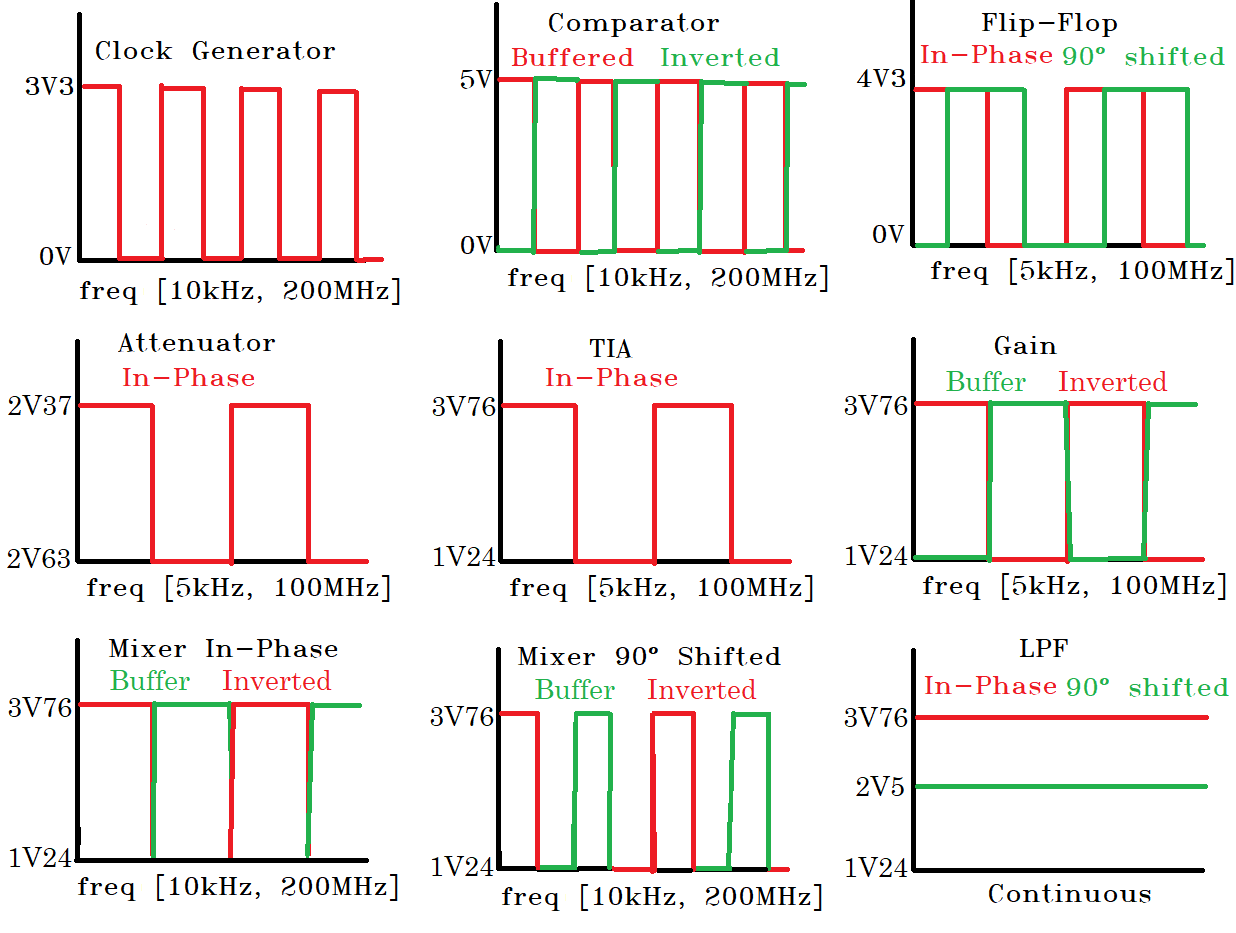
\includegraphics[width=1\textwidth]{IFCPracticalExample}
    \caption{Signal behavior for every electronical modules of the impedance-sensing device when measuring a 1k$\Omega$ resistor with a 10k$\Omega$ feedback resistor at the PGA.}
    \label{fig:IFCPracticalExample}
\end{figure}
By calculating the difference of these signals from the middle of the power-supplies, it is possible to obtain the real and imaginary components. the real component is 1.265 while the imaginary component is 0. Since the SUT in this case is a resistor, which has only a real component for the impedance, the conversion from the square spectroscopy to a sine spectroscopy doesn't modify the results, as described in the proof below. 
\begin{proof}
Since this is a 1k$\Omega$ resistor, the real component should be 1000 and the imaginary component should be 0. 
    \begin{align*}
        \Re(V_{PSD-\omega_0}) & = \frac{1}{2}\frac{6}{\pi^2} \frac{V_0 R_f}{A} \displaystyle\sum_{n=1,3,5,7...} ^{\infty} \frac{\cos(\theta(n \omega_0))}{n^2\lvert Z \rvert (n \omega_0)}\nonumber\\
        1.265 & = \frac{1}{2} \frac{6}{\pi^2} \frac{4.3 * 4 700}{17} \displaystyle\sum_{n=1,3,5,7...} ^{\infty} \frac{\cos(0 ^\circ)}{n^2 1000}\nonumber\\
        1.265 & = \frac{1}{2} \frac{6}{\pi^2} 2529 \displaystyle\sum_{n=1,3,5,7...} ^{\infty} \frac{1}{n^2 1000}\nonumber\\
        1.265 & = \frac{1}{2} \frac{2529}{1000}\nonumber\\ 
        1000 & = 1000\nonumber &&\qedhere
    \end{align*}
\end{proof}
\autoref{eq:CorrectedMagnitude} and \autoref{eq:CorrectedPhase} can thus be used directly with \autoref{eq:RealPSD} and \autoref{eq:ImPSD} to calculate the magnitude and phase of the SUT's impedance. A magnitude of 1000$\Omega$ and a phase of 0$^\circ$ are calculated, which is exactly what was sought for the 1k$\Omega$ resistor.  \par

\subsection{General example}
Another more general example can be illustrated for a complex system involving a series capacitor and resistor of values 1nF and 1k$\Omega$ excited by an input square signal of frequency 100kHz with a transimpedance of the PGA of 10k$\Omega$. The impedance magnitude and phase of the SUT would then be 1880$\Omega$ and -57.86 $^\circ$. Here is the proof below:

\begin{proof}
    Knowing that the impedance magnitude and phase for the fundamental and three first harmonics are: ($n=1$) 1880$\Omega$ and -57.86 $^\circ$, ($n=3$) 1132$\Omega$ and -27.95 $^\circ$, ($n=5$) 1049$\Omega$ and -17.66 $^\circ$, ($n=7$) 1025$\Omega$ and -12.81 $^\circ$. The real and imaginary components sampled by the ADCs would be:
    \begin{align*}
       \Re(V_{PSD-\omega_0}) &= \frac{1}{2} \frac{6}{\pi^2} \frac{V_0 R_f}{A} \displaystyle\sum_{n=1,3,5,7...} ^{\infty} \frac{\cos(\theta(n \omega_0))}{n^2\lvert Z \rvert (n \omega_0)}\nonumber\\
        &= \frac{1}{2} \frac{6}{\pi^2} 2529 [\frac{\cos(57.86 ^\circ)}{1880} + \frac{\cos(27.95^\circ)}{3^2 * 1132} + \frac{\cos(17.66 ^\circ)}{5^2 * 1049} + \frac{\cos(12.81 ^\circ)}{7^2 * 1025} + \dots]\nonumber\\
        &= -0.2350 \nonumber
       \end{align*}
     \begin{align*}
       \Im(V_{PSD-\omega_0}) &= \frac{1}{2} \frac{6}{\pi^2} \frac{V_0 R_f}{A} \displaystyle\sum_{n=1,3,5,7...} ^{\infty} \frac{\sin(\theta(n \omega_0))}{n^2\lvert Z \rvert (n \omega_0)}\nonumber\\
        &= \frac{1}{2} \frac{6}{\pi^2} 2529 [\frac{\sin(57.86 ^\circ)}{1880} + \frac{\sin(27.95^\circ)}{3^2 * 1132} + \frac{\sin(17.66 ^\circ)}{5^2 * 1049} + \frac{\sin(12.81 ^\circ)}{7^2 * 1025} + \dots]\nonumber\\
        &= 0.1991\nonumber
    \end{align*}
    Now these real and imaginary square components must be corrected using the rules described in \citep{Subhan2019} following \autoref{eq:correctionReal}. The coefficients $\Re(V_{PSD-\omega_0})$ and $\Im(V_{PSD-\omega_0})$ at the harmonics frequency must have been sampled beforehand. $\Re(V_{PSD-3\omega_0}=-0.4865$, $\Re(V_{PSD-5\omega_0}=-0.5489$, $\Re(V_{PSD-7\omega_0}=-0.5698$, $\Im(V_{PSD-3\omega_0}=0.1906$, $\Im(V_{PSD-5\omega_0}=0.1332$, $\Im(V_{PSD-7\omega_0}=0.0994$. 
    \begin{align*}
       \Re(V_{sine-\omega_0}) &= \frac{1}{2} \frac{6}{\pi^2} \frac{V_0}{A} R_f [ \displaystyle\sum_{n=1,3,5,7...} ^{\infty} \frac{\cos(\theta(n \omega_0))}{n^2\lvert Z \rvert (n \omega_0)} - \displaystyle\sum_{n=3,5,7...} ^{\infty} \frac{\cos(\theta(n \omega_0))}{n^2\lvert Z \rvert (n \omega_0)}]\nonumber\\
       &= \Re(V_{PSD-\omega_0}) - \frac{1}{3^2}\Re(V_{PSD-3\omega_0}) - \frac{1}{5^2}\Re(V_{PSD-5\omega_0}) - \frac{1}{7^2}\Re(V_{PSD-7\omega_0}) + \dots\nonumber\\
       &=  -0.2350 + \frac{0.4865}{9} + \frac{0.5489}{25} + \frac{0.5698}{49} + \dots\nonumber\\
       &= -0.1474\nonumber
   \end{align*}
   \begin{align*}
       \Im(V_{sine-\omega_0}) &= \frac{1}{2} \frac{6}{\pi^2} \frac{V_0}{A} R_f [ \displaystyle\sum_{n=1,3,5,7...} ^{\infty} \frac{\sin(\theta(n \omega_0))}{n^2\lvert Z \rvert (n \omega_0)} - \displaystyle\sum_{n=3,5,7...} ^{\infty} \frac{\sin(\theta(n \omega_0))}{n^2\lvert Z \rvert (n \omega_0)}]\nonumber\\
       &= \Im(V_{PSD-\omega_0}) + \frac{1}{3^2}\Im(V_{PSD-3\omega_0}) - \frac{1}{5^2}\Im(V_{PSD-5\omega_0}) + \frac{1}{7^2}\Im(V_{PSD-7\omega_0}) + \dots\nonumber\\
       &=  0.1991 + \frac{0.1906}{9} - \frac{0.1332}{25} + \frac{0.0994}{49} + \dots\nonumber\\
       &= 0.2170\nonumber &&\qedhere
    \end{align*}
\end{proof}
The impedance magnitude is thus deduced the same way as the previous proof to be 1 837 $\Omega$, only 2.3\% away from the theoretical value of 1880 $\Omega$. The impedance phase is -55.8 $^{\circ}$, only 3.6\% away from the theoretical value of -57.86 $^\circ$. These errors are quite low considering that only the first 3 harmonics were subtracted from the square spectroscopy. When more harmonics are considered, the error can go as low as 1\% for the magnitude and 1.5\% for the phase.
\section{PCB design}
A four-layer PCB was conceived using Altium Designer and fabricated by PCBWay. It has a size of 50 $\times$ 50 $\times$ 15 mm including the components. The substrate is FR-4 TG150, with spacings of 6mils and a thickness of 1.5mm. The minimum holed size is 0.3mm with tented vias. Finally, the surface finish is HASL with lead with 1oz copper. The 3d-model and final PCB are shown in \autoref{fig:AltiumPCB} and \autoref{fig:PracticalPCB}. 
\begin{figure}[h]
\centering
\begin{subfigure}{0.49\textwidth}
\centering
    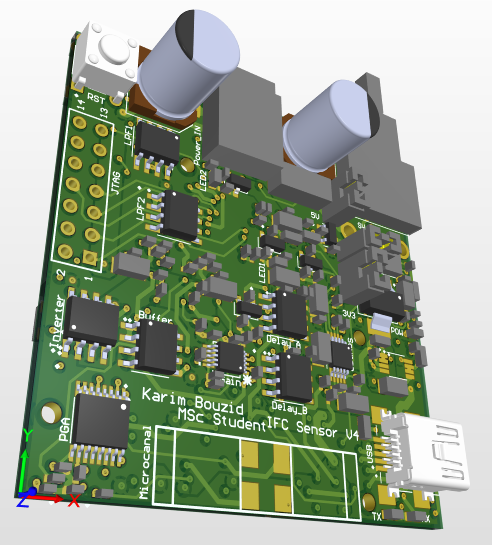
\includegraphics[width=0.9\linewidth]{PCB1}
    \caption{Front view.}
    \label{fig:PCB1}
\end{subfigure}
\begin{subfigure}{0.49\textwidth}
\centering
    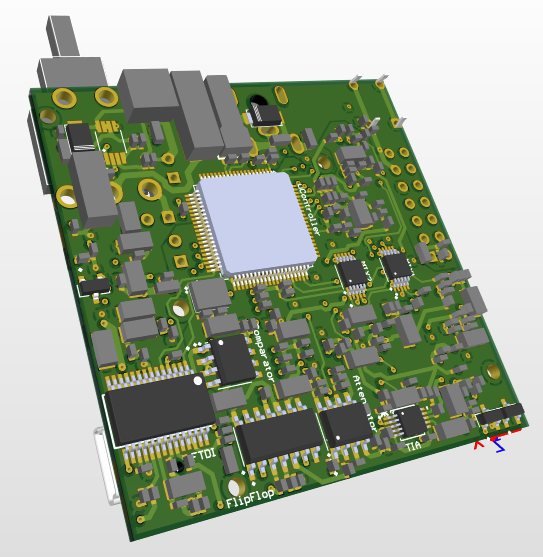
\includegraphics[width=0.96\linewidth]{PCB2}
    \caption{Back view.}
    \label{fig:PCB2}
\end{subfigure}
\caption{3d-model of the back and front views of the PCB as represented in Altium Designer.}
\label{fig:AltiumPCB}
\end{figure}
\begin{figure}[h]
\centering
\begin{subfigure}{0.49\textwidth}
\centering
    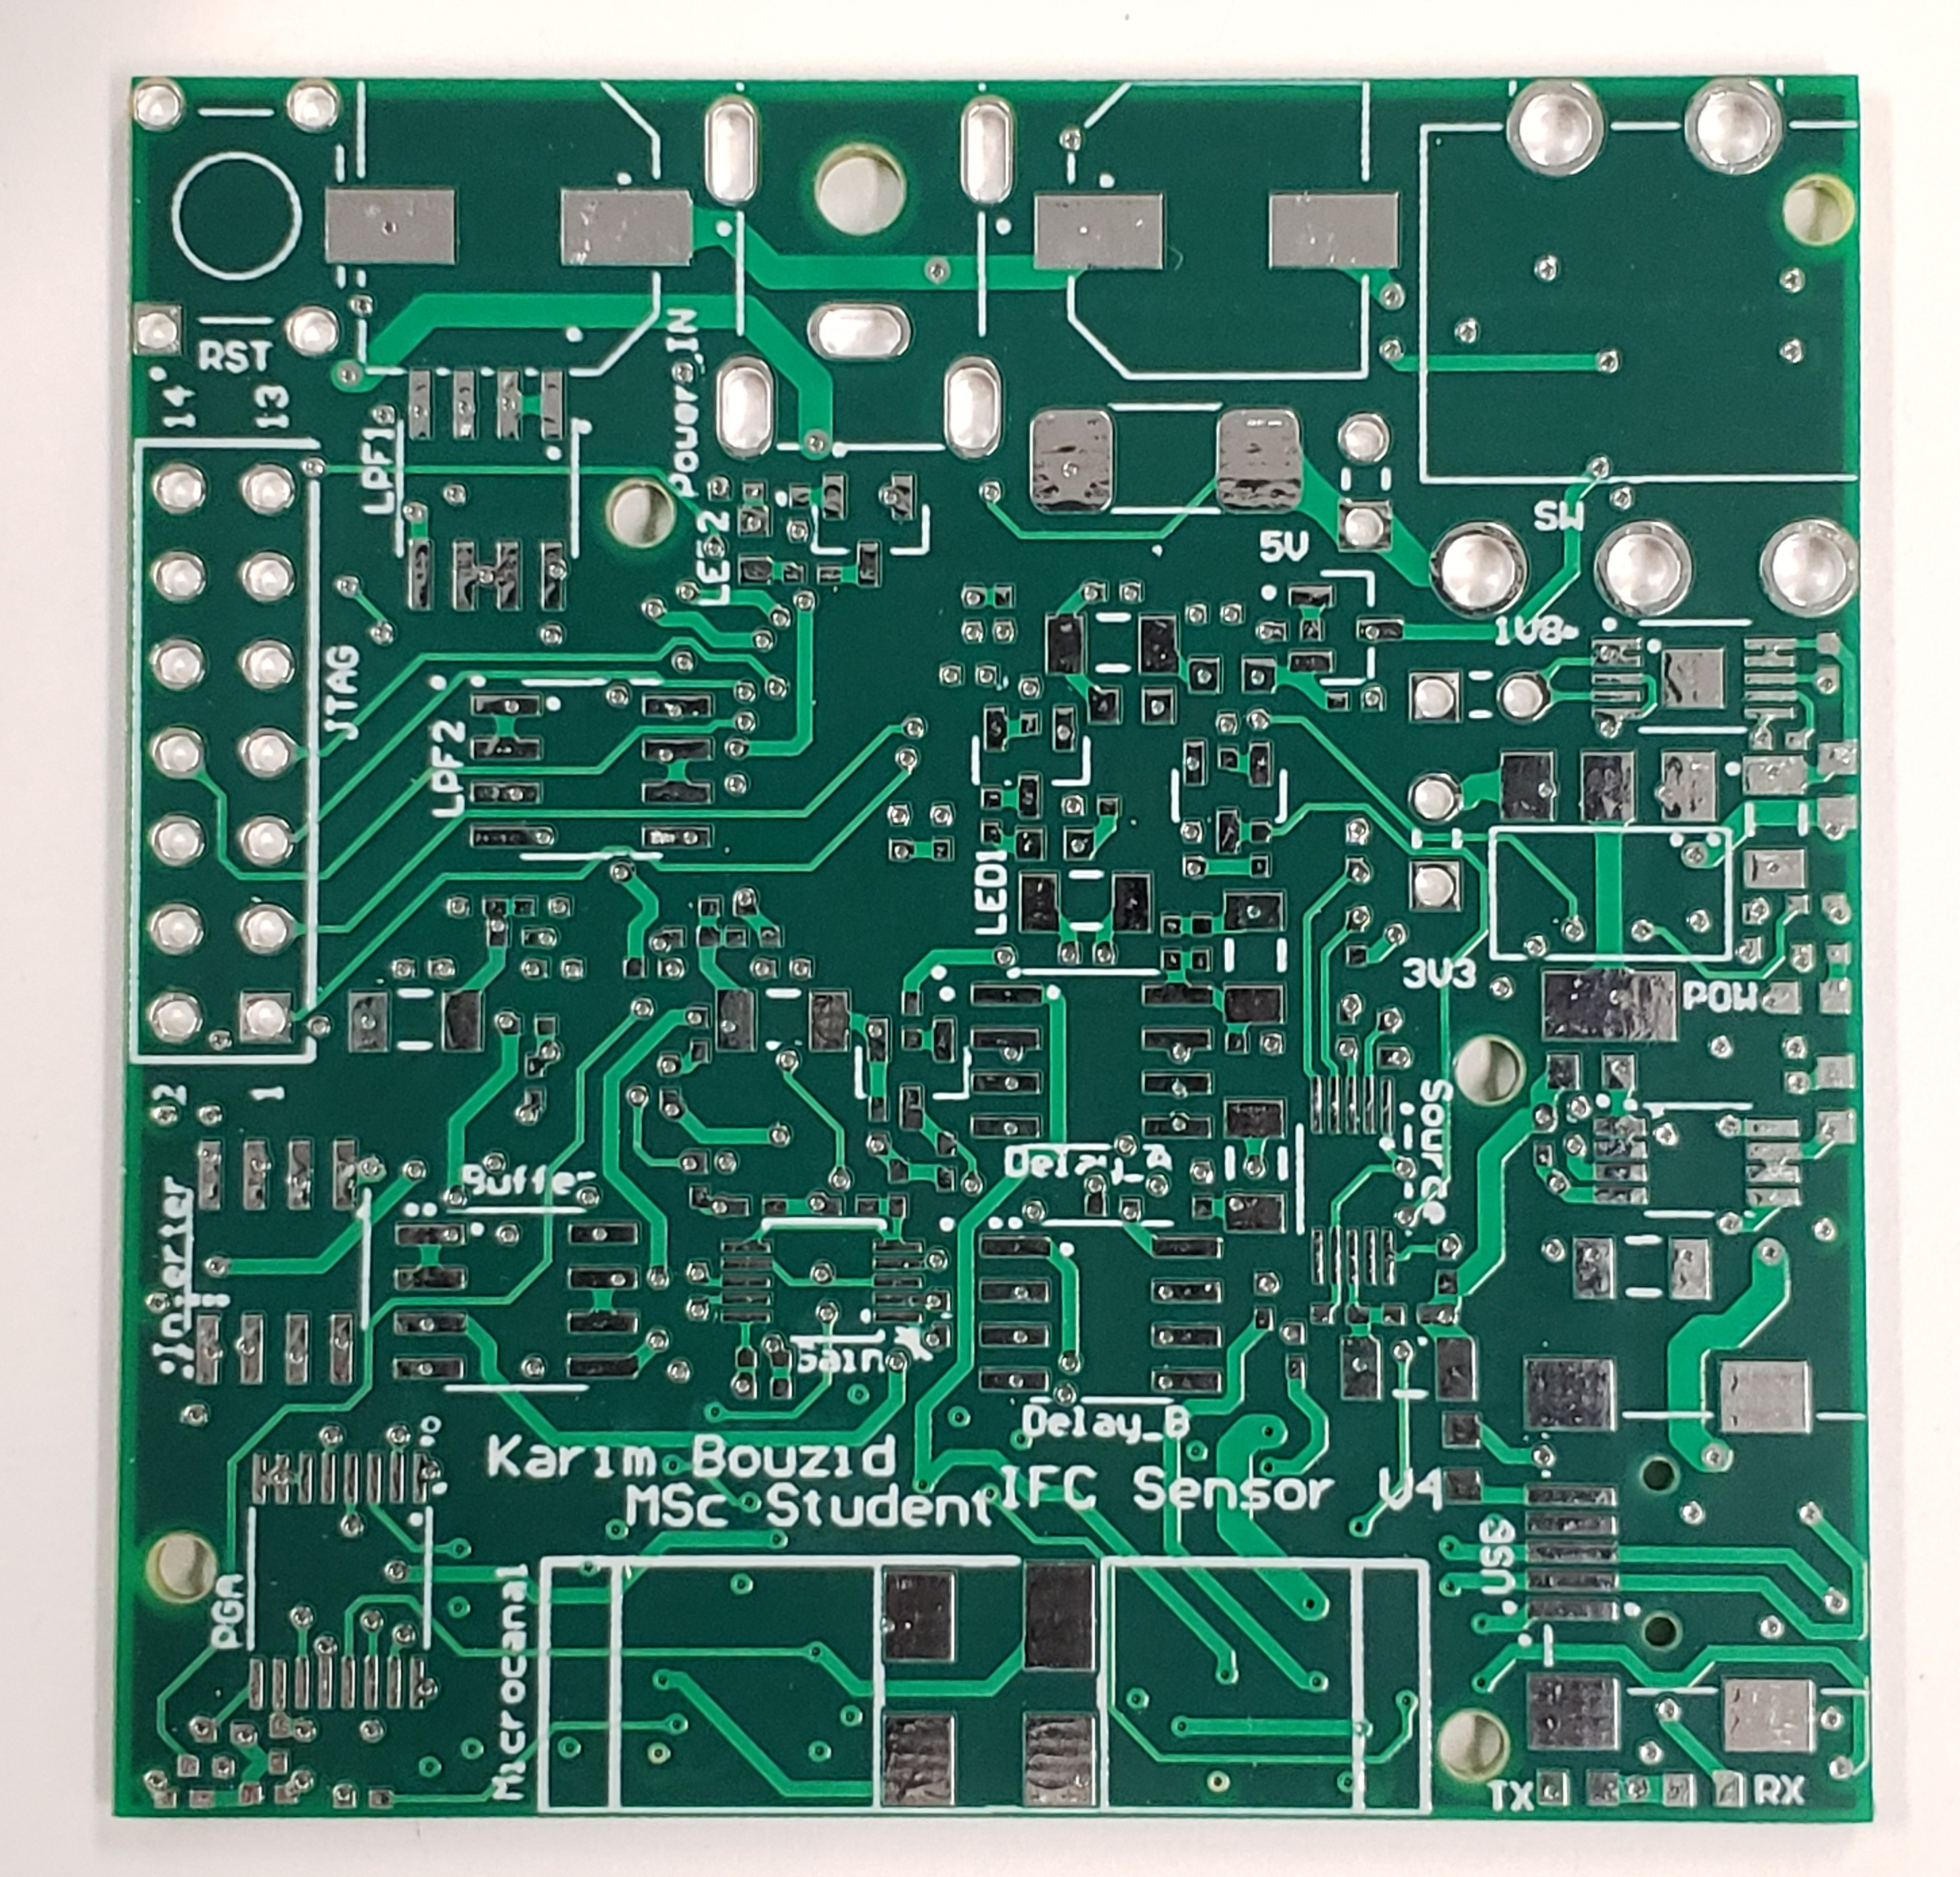
\includegraphics[width=1\linewidth]{BarePCB}
    \caption{Without components.}
    \label{fig:BarePCB}
\end{subfigure}
\begin{subfigure}{0.49\textwidth}
\centering
    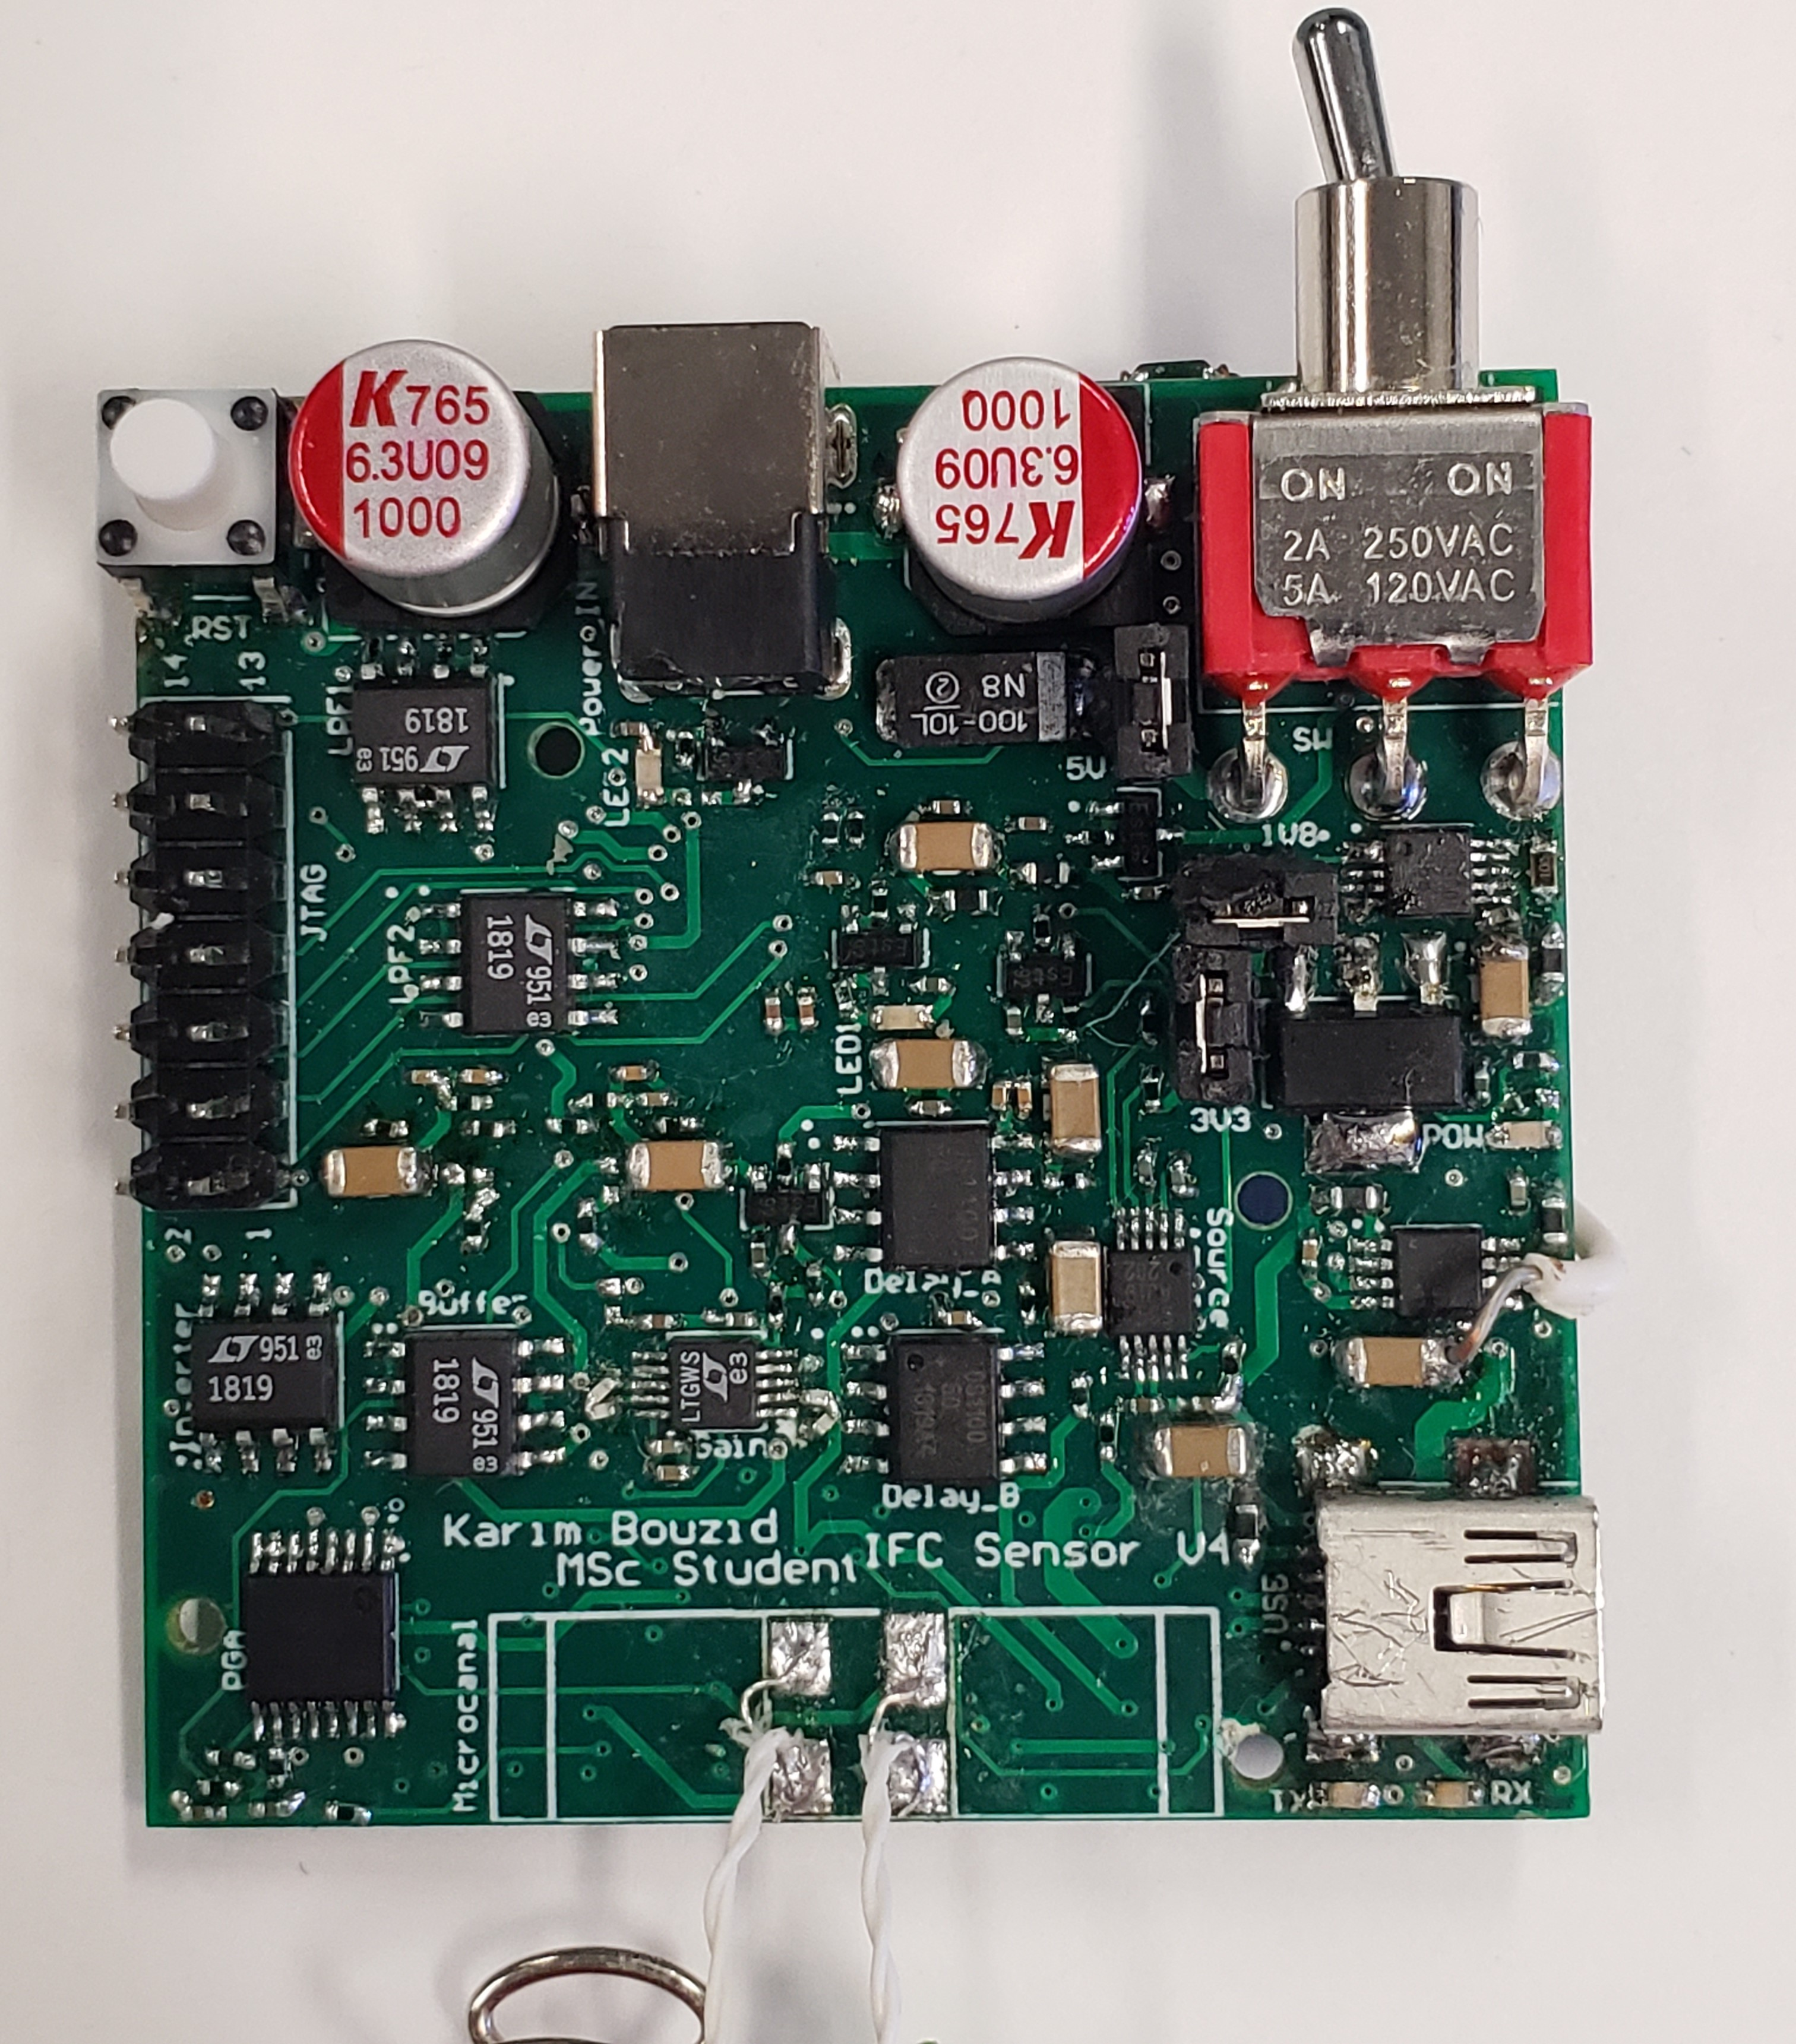
\includegraphics[width=0.85\linewidth]{FunctionalPCB}
    \caption{Soldered components.}
    \label{fig:FunctionalPCB}
\end{subfigure}
\caption{Front-view of the PCB.}
\label{fig:PracticalPCB}
\end{figure}
\section{MCU processes}
\label{sec:MCUprocesses}
The in-board microcontroller MSP430F5529 (see \autoref{sec:MCU}) executes multiple tasks in parallel. It can:
\begin{itemize}
    \item Enable or disable the power-supplies. 
    \item Monitor the status of the system by activating LEDs on the PCB. 
    \item Modify the gain of the PGA.
    \item Modify the phase of the quadrature-generator. 
    \item Modify the frequency of the square input voltage by programming the Si5351 IC. 
    \item Sample the real and imaginary components of the two electrode pairs current reponse $\Re(V_{PSD-\omega_0}$ and $\Im(V_{PSD-\omega_0}$ at high frequency. 
    \item Sample the voltage of the 5V $V_{DD}$ power-supply at high frequency, and the voltage of the battery at low-frequency. 
    \item Transfer the sampled data to a nearby computer with the help of a FT232RL IC. 
\end{itemize}

It is possible to modify on the fly some of the properties or behavior of the impedance-sensing system. Different commands can be transmitted to the MCU to modify the properties. These commands are shown in \autoref{fig:LoopFlowchart}. \par

The system can be operated in single or multi-frequency modes. The single frequency-mode samples data at a single input frequency. The multi-frequency mode modifies the excitation frequency from an initial frequency up to a maximum frequency each time the sample buffer is full, then it cycles back to the minimum frequency. This technique can be used to obtain the impedance spectroscopy (see \autoref{sec:EIS}) of the SUT. The data transfer can be paused or not. A low-power mode can toggle on if the system is unused for a period of time. Finally, the sampling rate of the system can be toggled between a low constant sampling frequency of 655Hz, and a variable rate high-speed sampling frequency of 5461Hz. \par
\begin{figure}[h]
    \centering
    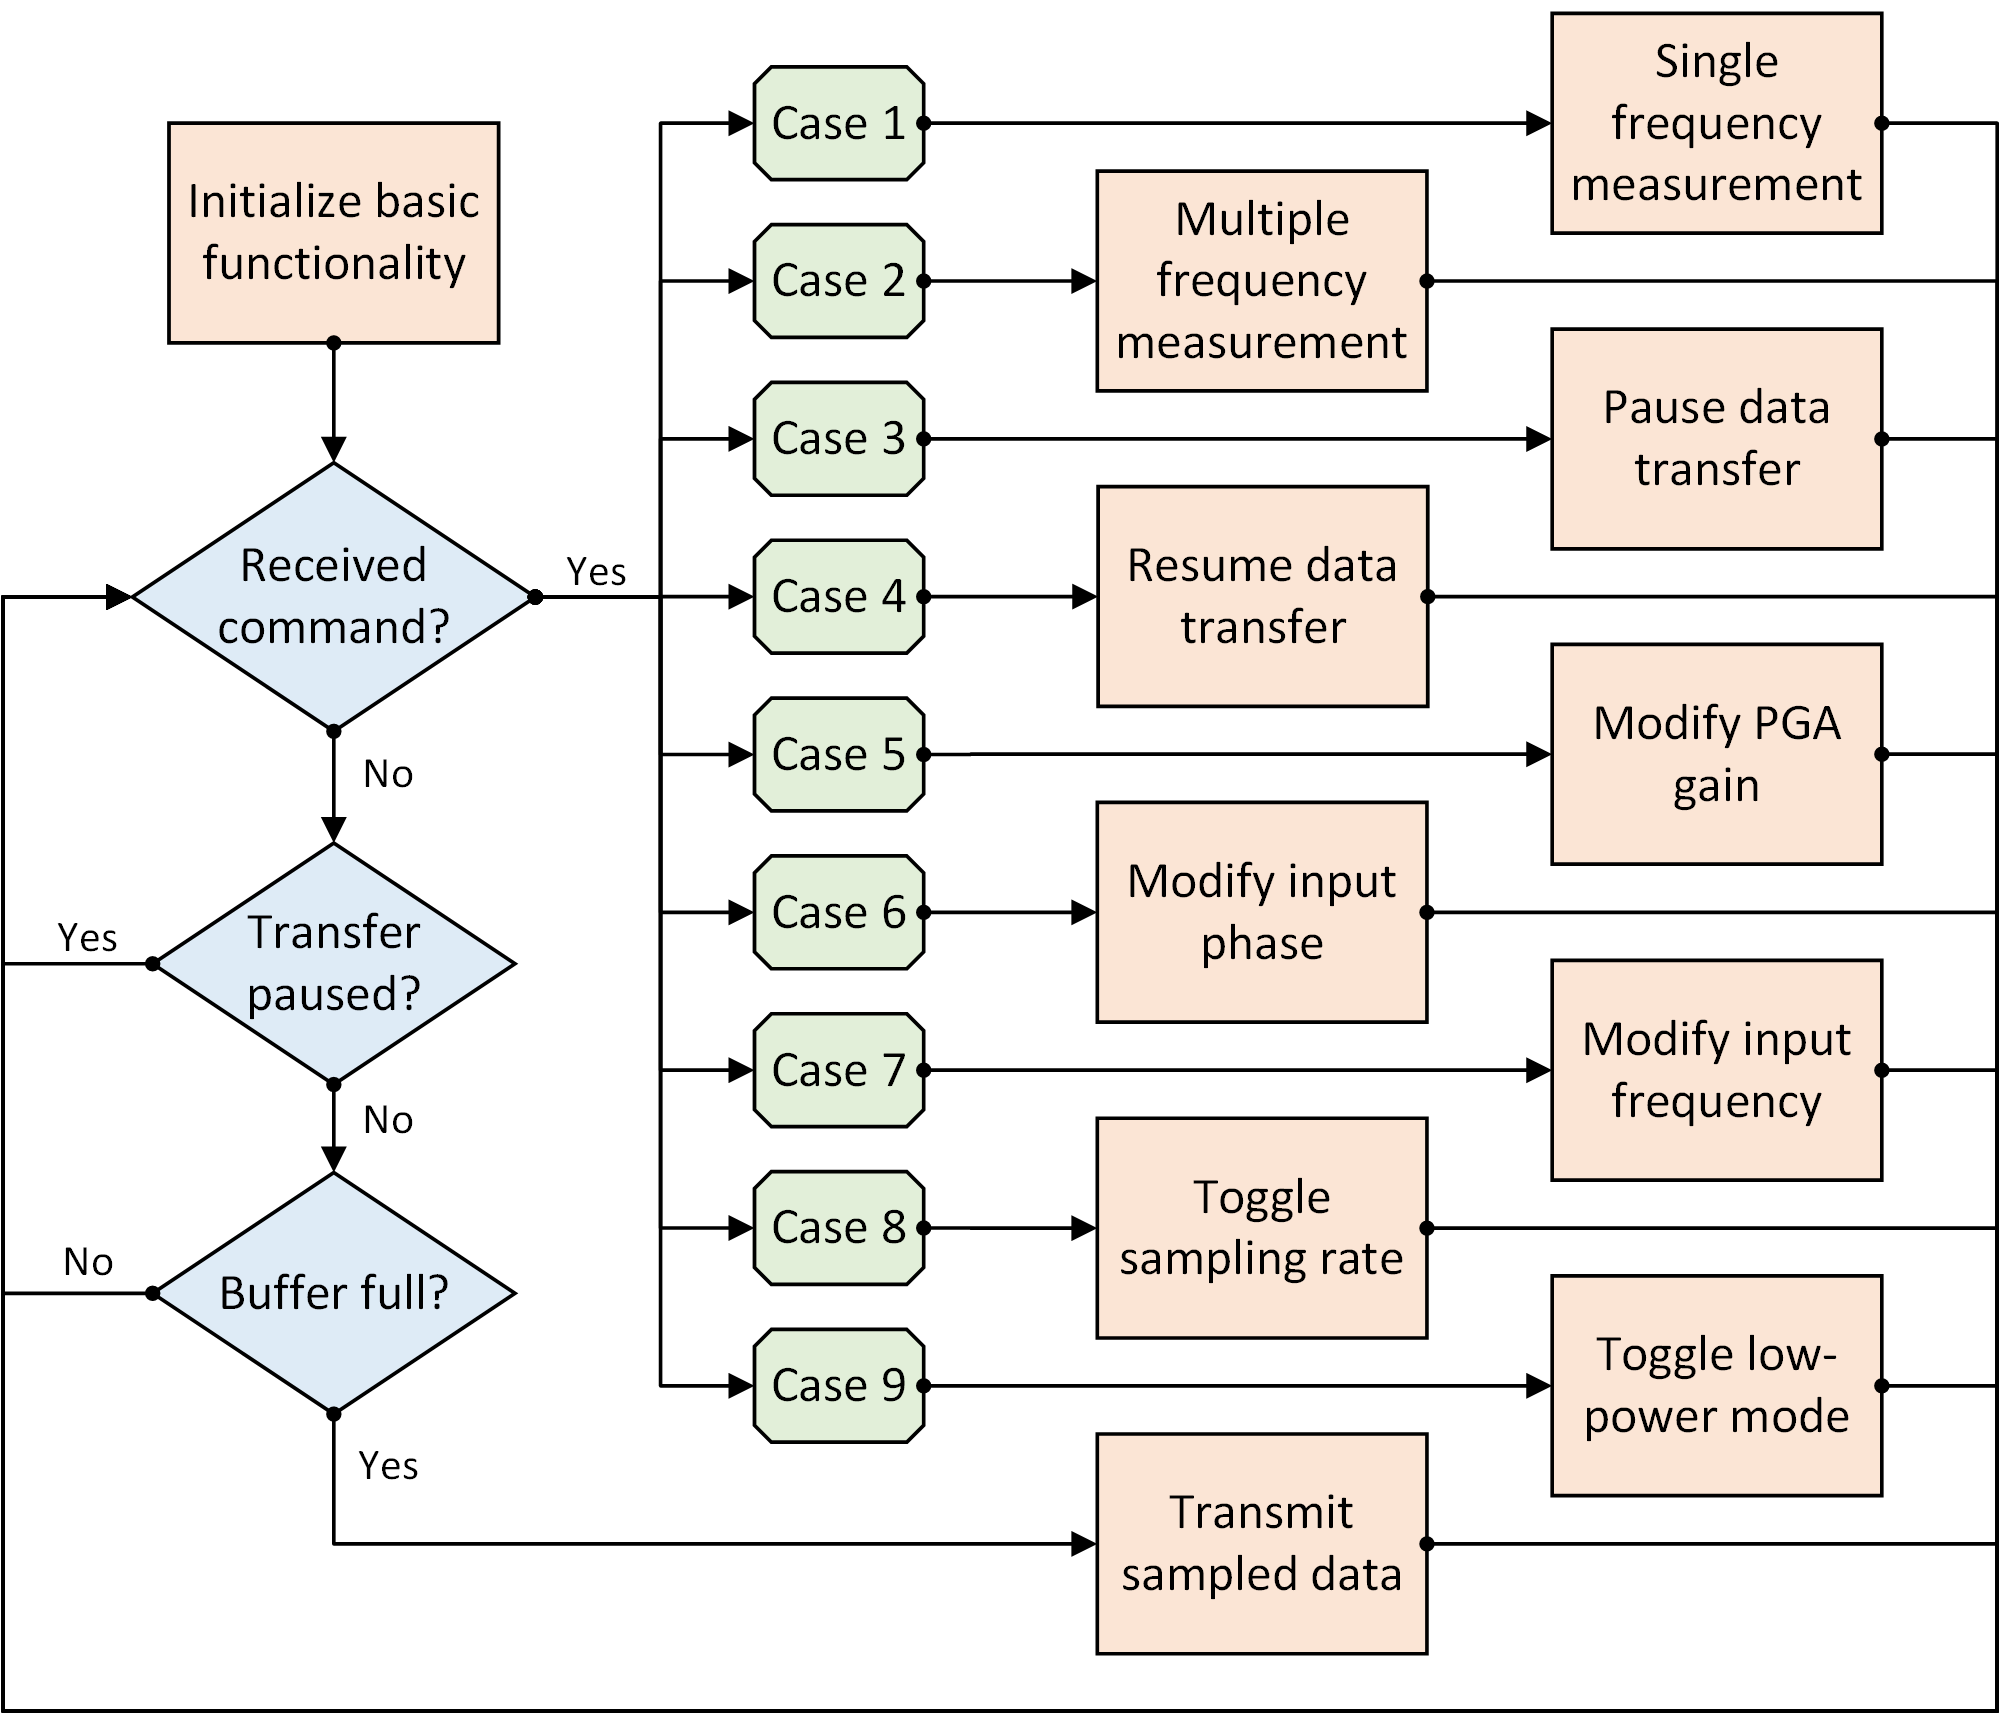
\includegraphics[width=0.95\textwidth]{LoopFlowchart}
    \caption{Flowchart of the MCU for the impedance-sensing system.}
    \label{fig:LoopFlowchart}
\end{figure}

The variable rate sampling works by sampling the data at a high frequency, and only putting the data in the sampling buffer if a significant difference is observed from the few previous samples. This technique is useful in IFC since only the half-sine waveform observed when a particle passes in the channel are useful for the detection. The impedance measured when no particles are in the channel is flat, and only serve to saturate the buffers, which limits the maximum sampling rate of the MCU. As an example, using a variable sampling rate to samples 64 consecutive data points only when a significant difference in measured data is observed increases the maximum practical sampling rate from 655Hz to 5461Hz. %The flowchart of the behaviors of the MCU during the interruptions is given in \autoref{fig:InterruptFlowchart}. \par

%\begin{figure}[h]
%    \centering
%    \includegraphics[width=0.8\textwidth]{InterruptFlowchart}
%    \caption{Flowchart of the interrupt of the MCU for the impedance-sensing system.}
%    \label{fig:InterruptFlowchart}
%\end{figure}



\chapter{Microfluidics}
\label{chap:Microfluidics}
Theoretical aspects of fluid dynamics will be described in this chapter. Practical designs to limit the quantity of air bubbles and other anomalies will also be described, as well as microfabrication techniques and a thorough description of the microfluidics system produced in this study.
\section{Fluid dynamics and design considerations}
When dealing with microfluidics, some important concepts should be kept in mind. The liquid flow should be kept as smooth as possible and be devoid of any flaws such as cross-current, eddies, swirls, or bubbles. In fluid dynamics, such a smooth flow state is called laminar flow and is characterized by an orderly movement of the particles within the liquid \cite{lagerstrom1996laminar,bruus2011theoretical}. The particles in that state move in straight lines parallel to the adjacent walls, and no mixing is observed between the flow layers. The reciprocal of laminar flow is called turbulent flow, and is observed at higher fluid speed and density, lower liquid viscosity, and for larger diameters of conduits (see \autoref{fig:LaminarTurbulent}. An important concept when defining the smoothness of a liquid flow is the Reynolds number. It is a dimensionless parameter that operates on the ratio of the inertial force to the shearing force of the flowing liquid. Its specific calculation depends on the geometry of the canal. For high Reynolds number, the flow is defined as turbulent, whereas it is defined as laminar for low Reynolds number \cite{lagerstrom1996laminar,bruus2011theoretical}. The density and viscosity of the liquid are parameters that are application specific, but the speed of the liquid and the diameters of the conduits are parameters that can be modified when designing a microfluidic sensor. Lower liquid velocity and smaller conduits should then be used to obtain a smooth laminar flow. \par
\begin{figure}[h]
    \centering
    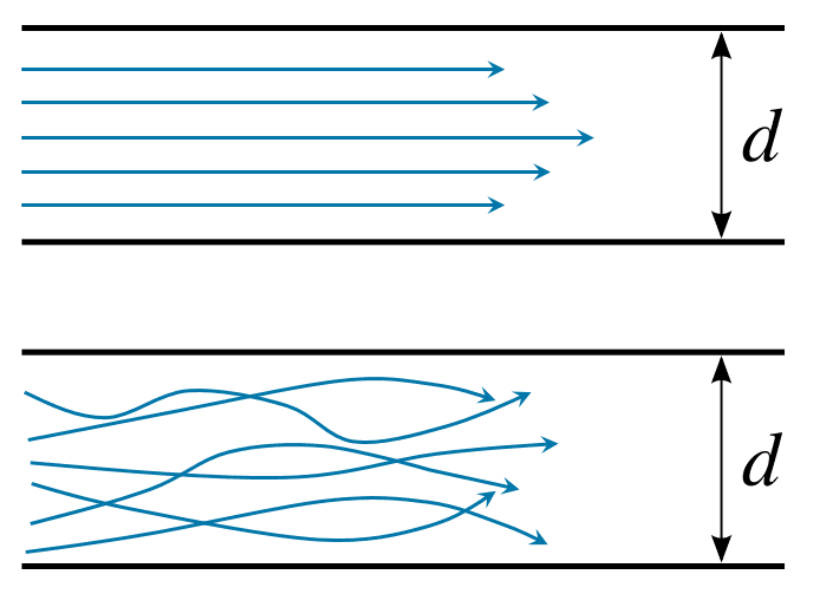
\includegraphics[width=0.5\textwidth]{LaminarTurbulent}
    \caption{Behavior of laminar [up] and turbulent [down] flow in a fluidic channel. \citep{simscale_2021}}
    \label{fig:LaminarTurbulent}
\end{figure}
The behaviors observed in microfluidics is analogous to those observed in electrical circuits: the current flow can be associated with the electrical current, the applied pressure with an applied ideal voltage source, and the resistance to the flow with the electrical resistance. Flow compliance, the analog of electrical capacitance, is also defined as the modification of the channel volume when an increase in pressure is observed \cite{bruus2011theoretical}. This generally happens for soft wall materials or when gas is compressed in the channel. Flow resistors are an important design consideration and can be adjusted by modifying the cross-section geometry and width, and length of the channel \cite{bruus2011theoretical,Olanrewaju2018}. \par

The capillary pressure is also affected by the geometry of the channel, meaning that such a variation is always associated with a decrease in flow rate and in flow speed (for $h<<w$, the flow rate is reduced in $\frac{1}{h^2}$ and the flow speed in $\frac{1}{h}$ \cite{lagerstrom1996laminar,bruus2011theoretical}. The flow rate follows a Poiseuille-Flow for low Reynolds number and laminar flow when applied with a pressure difference $\Delta P$ between its inlet and outlet, which is a parabolic fluid velocity across the circular channel cross-section, with a maximum velocity at the center and null-speed near the walls. To calculate the flow rate $Q$ in a microfluidic system, it is necessary to solve the Stockes equation, which can be rendered geometry independent using the flow resistor as a parameter \cite{bruus2011theoretical,Zimmermann2007}: 
\begin{equation}
   Q = \frac{1}{\nu} \frac{\Delta P}{R_f}
\end{equation}
Where $\nu$ is the viscosity of the liquid, $\Delta P$ the difference in pressure inside and in front of the liquid, and $R_f$ the total resistance to flow. It is important to note that since the flow rate depends on the viscosity, the flow resistance will increase as the gas present in the channel at the beginning is replaced by a liquid \cite{bruus2011theoretical,Zimmermann2007}. \par

The pressure difference in the microchannel $\Delta P$ can be created using capillary pump based on the Young-Laplace equation. Such pumps can however only hold nanoliters of liquid and induce flow rates in the nanoliters per seconds, meaning they are more suitable for immunoassay analysis than for long-term tests. These pumps are created using intricate channel geometries that maximize the pressure difference. This is often done by maximizing the liquid contact regions with the channels walls and by reducing the width and height of the conduits, such as in “tree lines”, “hexagons”, and “balled lines” geometries \cite{bruus2011theoretical,Zimmermann2007}. \par

Syringes are often used in microfluidics application despite some shortcomings. They create a pressure difference between the inlet and outlet, which is associated to a flow rate flow, flow resistance, and compliance of the channel \cite{SyringePumps,bruus2011theoretical}. The soft material generally used in microfluidics, such as the tubing made from Tygon, channel made in PDMS, plastic syringes, etc. get deformed when confronted to a pressure difference, which induces a compliance in the channel. This compliance, when associated to the channel resistance, creates a settling time analogous to the settling times of RC systems in electronics. This means that the systems lose in responsiveness when using syringe pumps, with the flow rate linearly increasing over a settling time after a pressure change is applied. The experiments using syringe pumps thus lose in responsiveness and reproducibility compared to those using more advanced microfluidic pressure controller \cite{SyringePumps,Olanrewaju2018,bruus2011theoretical}. \par

The wettability of surfaces is an important parameter in microfluidic applications since it governs the contact angle between the surface and the liquid. A surface is considered wettable in theory when the contact angle is less than 90° \cite{Olanrewaju2018}. Wettable surfaces, also call hydrophilic surfaces, generate a concave interface between liquid and gas, with a negative capillary pressure that sucks liquids inside the channel. Hydrophobic surfaces, on the other hand, are defined for contact angles higher than 90°. They create a convex interface between liquid and gas, and a positive pressure which pushes liquid out of the channel. These interactions are depicted in \autoref{fig:Surface_Wettability}. It is important to note that these liquid-solid interfaces are unaffected by gravity since surface forces are dominant compared to inertial forces in capillary channels. In practice, imperfections in the conduit can drastically modify the wettability and capillary pressure inside the channel, which can disrupt the channel’s functionality. Contact angles below 60° are thus chosen for adequate flowing and since contact angles close to 90° are associated with high capillary pressures which block the liquid flow [41]. This relation can be expressed by the Young-Laplace equation \cite{Olanrewaju2018,bruus2011theoretical}:
\begin{figure}[h]
    \centering
    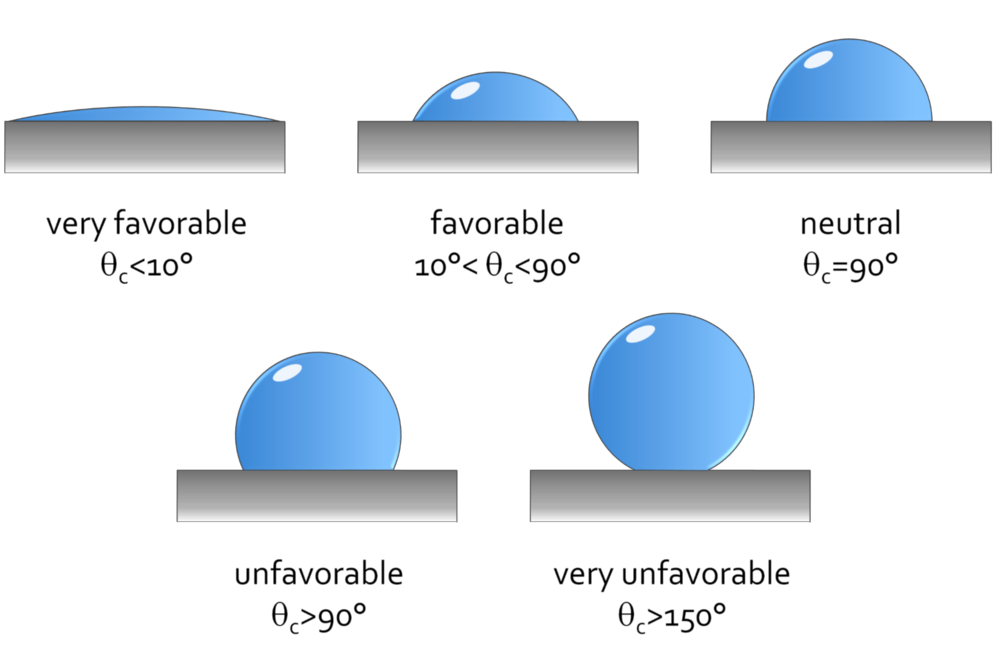
\includegraphics[width=0.8\textwidth]{Surface_Wettability}
    \caption{A droplet tend to cling to wettable surfaces, whereas it rolls off unwettable ones. \citep{surfacewettability}}
    \label{fig:Surface_Wettability}
\end{figure}
\begin{equation}
   \Delta P = -\gamma [\frac{cos(\theta_t)+cos(\theta_b)}{h} + \frac{cos(\theta_l)+cos(\theta_r)}{w}]
\end{equation}
where $\Delta P$ is the capillary pressure, $\gamma$ is the surface tension of liquid in the microchannel, $h$ and $w$ are the channel height and width respectively, and $\theta_t$, $\theta_b$, $\theta_l$, $\theta_r$ are the top, bottom, left, and right contact angles of liquid with the corresponding four microchannel walls \cite{Olanrewaju2018,bruus2011theoretical}. \par

Having contact angles lower than 60° on all walls often proves to be a challenging task since microchannels are generally made from heterogeneous materials. A sealing layer is often used, which features different fluidic properties than the rest of the conduit. The aspect ratio between $h$ and $w$ must then be chosen carefully as to not block the liquid flow when a hydrophobic material is used \cite{Olanrewaju2018}.\par

Additionally, the contact angle should always be kept higher than 30° to reduce the impacts of corner flow, which happens when a liquid flows between two surfaces with different contact angles. The liquid on the side of the most hydrophilic wall will precede the bulk flow. This may create deviations to the pressure predicted with the Young-Laplace equation and affect the uniform wetting of sensor electrodes \cite{Olanrewaju2018}. \par

Glass and silicon dioxides, two materials of choice for lithography-based microfluidic systems, have contact angles of 25° and 52°, respectively, making them both hydrophilic. PDMS, the leading substrate for quick prototyping, is, on the other hand, hydrophobic with a contact angle of 107° \cite{Olanrewaju2018,Trantidou2017}. Surface treatment is thus necessary to render it sufficiently wettable for use in capillary microchannels. The most common way to wet a surface is by exposing it to highly reactive plasma, ozone, or UV light \cite{Ufluidix}. High energy radicals are thus created and oxidize the surface, increasing its wettability. However, such treatments only modify the surface for a short while: 10min in the case of plasma. \citep{Trantidou2017} grafted silanes such as polyethylene glycol (PEG) or Polyvinyl alcohol (PVA) with hydrophilic end groups unto the PDMS surface after plasma treatment via heat immobilization to stabilize the surface wettability up to 30 days, with contact angles staying between 30° and 60°\cite{Olanrewaju2018,Ufluidix,Trantidou2017}. 
\section{Bubbles in microfluidics systems}
Bubbles present in the channels can significantly disrupt the good functioning of the sensor. These perturbations may range from (1) Flow-rate instability if the air bubbles are dilating/contracting \cite{AirBubbles,bruus2011theoretical,Kang2010}. (2) An increase in flow compliance caused by the absorption of pressure changes in the bubbles \cite{AirBubbles,bruus2011theoretical}. (3) An increase in the flow resistance since the bubbles reduce the width of the channel \cite{AirBubbles}. (4) Damages to the cell culture caused by the interfacial tension between the bubble and the liquid which may even result in cell death \cite{AirBubbles,Kang2010}. (5) Aggregation of particles at the interfaces \cite{AirBubbles}. (6) Damage to the wall functionalization of the channel \cite{AirBubbles,Kang2010}. \par

Although they are known to be recalcitrant, some techniques can be used to minimize their impact.  Before dealing with the bubbles, it is important to know their origin in the microfluidics setup and how they form. (1) Some residual bubbles may lodge themselves in the channel after filling it with liquid \cite{bruus2011theoretical,AirBubbles}. (2) Some may be introduced when mixing a second liquid in the channel \cite{AirBubbles}. (3) Some may be induced by porous materials such as PDMS\cite{AirBubbles}. (4) Leaks in the microfluidics setup may introduce bubbles \cite{AirBubbles}. (5) Dissolved gas in the liquid may create them, especially if a surfactant such as soap is mixed with the liquid, or if the liquid is heated, considering that higher temperature presents a lower gas solubility. \cite{AirBubbles,Ufluidix}. \par

Bubbles form themselves from a nucleation point, such as a small irregularity on the surface in which gas can be trapped or regions of low wettability. The nucleation point creates a region of gas phase stability at normal conditions of temperature and pressure \cite{Ufluidix}. When an external pressure is applied, the accumulated gas will either dissolve or expand if the critical radius to form a bubble is reached.  This produces a net growth of the gas in the nucleation point, which may dislodge itself to form a free-moving bubble \cite{Ufluidix,bruus2011theoretical}. The nucleation point will stay in place afterward, generating new bubbles. \par
\begin{figure}[h]
    \centering
    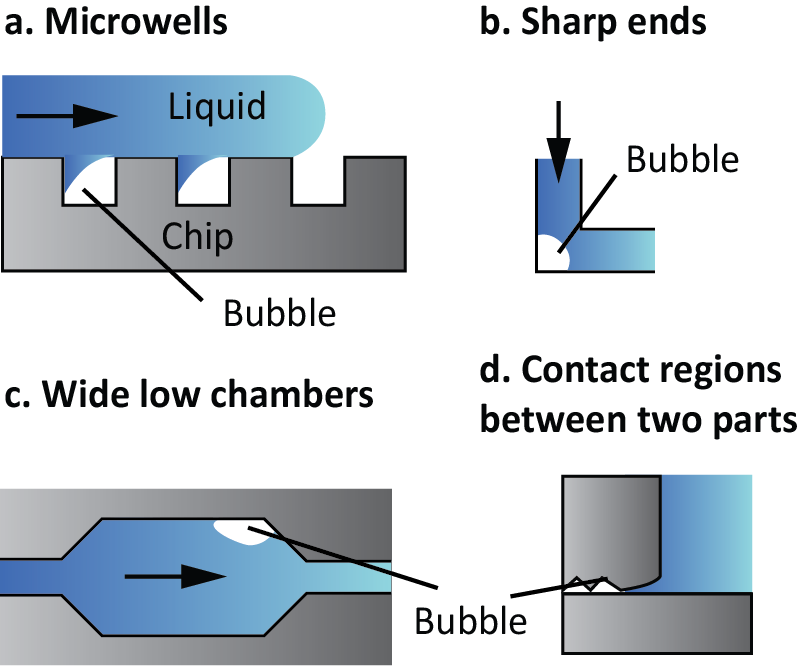
\includegraphics[width=0.7\textwidth]{AirBubble}
    \caption{Origins of air bubbles in a microfluidic channel. \citep{Ufluidix}}
    \label{fig:Airbubble}
\end{figure}
Being aware of their origins, as shown in \autoref{fig:Airbubble}, it is now possible to instigate preventive measures when designing the microfluidic chip to reduce the impacts of the bubbles. (1) Acute angles in the channel should be avoided since bubbles tend to adhere to corners. Dead ends, microwells, and sharp corners should thus be avoided \cite{AirBubbles,Ufluidix}. (2) The channel should be sealed tight using adequate fittings, and contact regions between two separate parts of the device should be bonded adequately, even using Teflon tape or a cladding material such as glues or epoxy if needed \cite{AirBubbles,Ufluidix}. (3) The liquids should be degassed prior to the experiment \cite{AirBubbles}. (4) The surfaces of the channel should be wet to contact angles below 60° to decrease the chance of bubbles getting trapped under sharp angles \cite{Olanrewaju2018,Ufluidix}, and above 30° to prevent corner flow. Corner flow happens when two surface with different wettability composes the walls of a channel. The liquid will flow quicker on some of the wall, resulting in an unequal flow which might create bubbles or even disrupt the channel’s function \cite{Olanrewaju2018}. (5) Pillar-like structures can be added to equalize the speed of the liquid front \cite{Ufluidix}. (6) Wide low chambers or any modification to the width of the channel should be avoided, as liquid tend to circulate at different speed at both sides of the chamber \cite{Ufluidix}. (7) Minimize the number of connectors as they add potential nucleation points for bubbles \cite{Ufluidix}.\par

Despite taking such precautions, bubbles may still remain a problem. In such case, corrective measures should be taken during the experiment. (1) Increasing the pressure inside the channel or sending pressure pulses might be sufficient to dislodge or dissolve the bubbles. Liquid under high pressure present a higher gas solubility \cite{AirBubbles,Ufluidix,bruus2011theoretical}. (2) Applying a higher pressure at both inlet and outlet might be sufficient to dissolve the bubbles into the channel material \cite{AirBubbles,Ufluidix}. (3) Adding degassing systems such as bubble traps or bubble detector to the channel. Some channel geometries have been demonstrated to help trapping or dissolving bubbles. Permeable materials also work to capture bubbles. Finally, hydrophobic materials tend to capture bubbles \cite{AirBubbles,Ufluidix,Olanrewaju2018,bruus2011theoretical,Kang2010}. (4) Flushing the channel with ethanol or a mix of ethanol and water before the experiment can help to remove stuck bubbles, since ethanol has a lower wetting angle than water \cite{Ufluidix}. \par

Bubble traps can be created only by adding cylindrical or hemispherical shapes in the channel path, although hemispherical ones were found to offer superior performances, consistently keeping a higher bubble occupation ratio \cite{Kang2010}. Such traps can be called active or passive depending on if they dissipate the bubbles or merely trap them in the channel. Active bubble traps have the advantage of performance, since the bubbles are taken out of the channel, but they require complex peripheral modules such as vacuum pumps to operate \cite{AirBubbles,Ufluidix,Kang2010}. The passive traps can also dissipate bubbles when an external pressure is applied if they are used in a porous channel substrate such as PDMS. Passive traps only work for hydrophobic surfaces. When used in hydrophilic ones, the bubbles simply slide off the surfaces of the channel when any external pressure is applied \cite{Kang2010}.
\section{Microfabrication techniques}
\label{sec:FabricationMicrofluidics}
Microfluidic channels can be fabricated using different techniques. The one producing the best resolution (around 2µm), which is also the most popular in research, is photolithography in cleanrooms \cite{Olanrewaju2018}. Direct patterning of the channels on silicon substrates can also be done using deep reactive ion etching. Soft lithography can also be chosen to reduce the mask price, at the cost of a decrease in resolution (around 10µm for plastic masks). A mold can be created and PDMS can be casted on that mold to create a channel using only an oven and simple consumable \cite{Olanrewaju2018}. A final sealing layer of glass or even PDMS can be used to seal tight the channel and the mold can be reused. This technique unfortunately requires expensive cleanroom facilities, complex fabrication processes, and high fabrication times \cite{Olanrewaju2018}. PDMS replication is adequate for academic settings (approximately 4h) but is too slow and uneconomic for industrial processed, which can achieve channels in minutes using hot embossing, or even in a couple of seconds using injection molding. 3d-printing can also be used to create molds in which PDMS can be cured. Multiple 3d-printing currently exist, but the one providing the best results for high resolutions and low surface roughness is stereolithography-based 3d-printing \cite{Olanrewaju2018,Gong2017}. UV light is applied to a resin basin, which incrementally moves in the z-axis. The resin is cured in layers and replicates a 3d-model designed on CAD software. The smallest feature produced using this technique is around 90µm, despite the resolution being claimed by manufacturer to be around 30µm. This can be explained because of the resin used these applications that tend to spread during curing, meaning that they are not especially suitable for microfluidics application \cite{Olanrewaju2018,Gong2017}. Recently, \citep{Gong2017} designed a homemade 3d-printer specifically for microfluidics which can attain truly microscopic scales of 18 x 20 µm by modifying the type of resin used and optimizing the stereolithographic process. 
\section{Practical microfluidic system}
\label{sec:PracticalMicrofluidic}
The microfluidic system made in this project is described in this section. It is defined as having an inlet and an outlet, where the liquid respectively enters and exits the device, fitted to soft Tygon thermoplastic tubing \cite{Olanrewaju2018}. The inlet tube is then linked to a glass syringe connected to a precise motor Syringe Pump by Cole-Parmer model CP-120 that compresses the syringe at a constant programmable rate. The SUT begins in the syringe, then flows in the tubes before entering the inlet. It then reaches the PDMS microchannel where it is sensed by the PCB electrodes linked to the Impedance Sensing Device. The liquid finally exits through the outlet tube, which is linked to a waste container. The PDMS channel and PCB electrodes are sealed tight by a system of 3d-printed squeezers that sandwich the channel and PCB electrodes together. Those are tightened together by screws, effectively sealing the microchannel and PCB electrode due to the flexible nature of PDMS. The microfluidic system is shown in \autoref{fig:MicrofluidicSystem} and illustrated in \autoref{fig:DiagramMicrofluidicSystem}. \par
\begin{figure}[h]
    \centering
    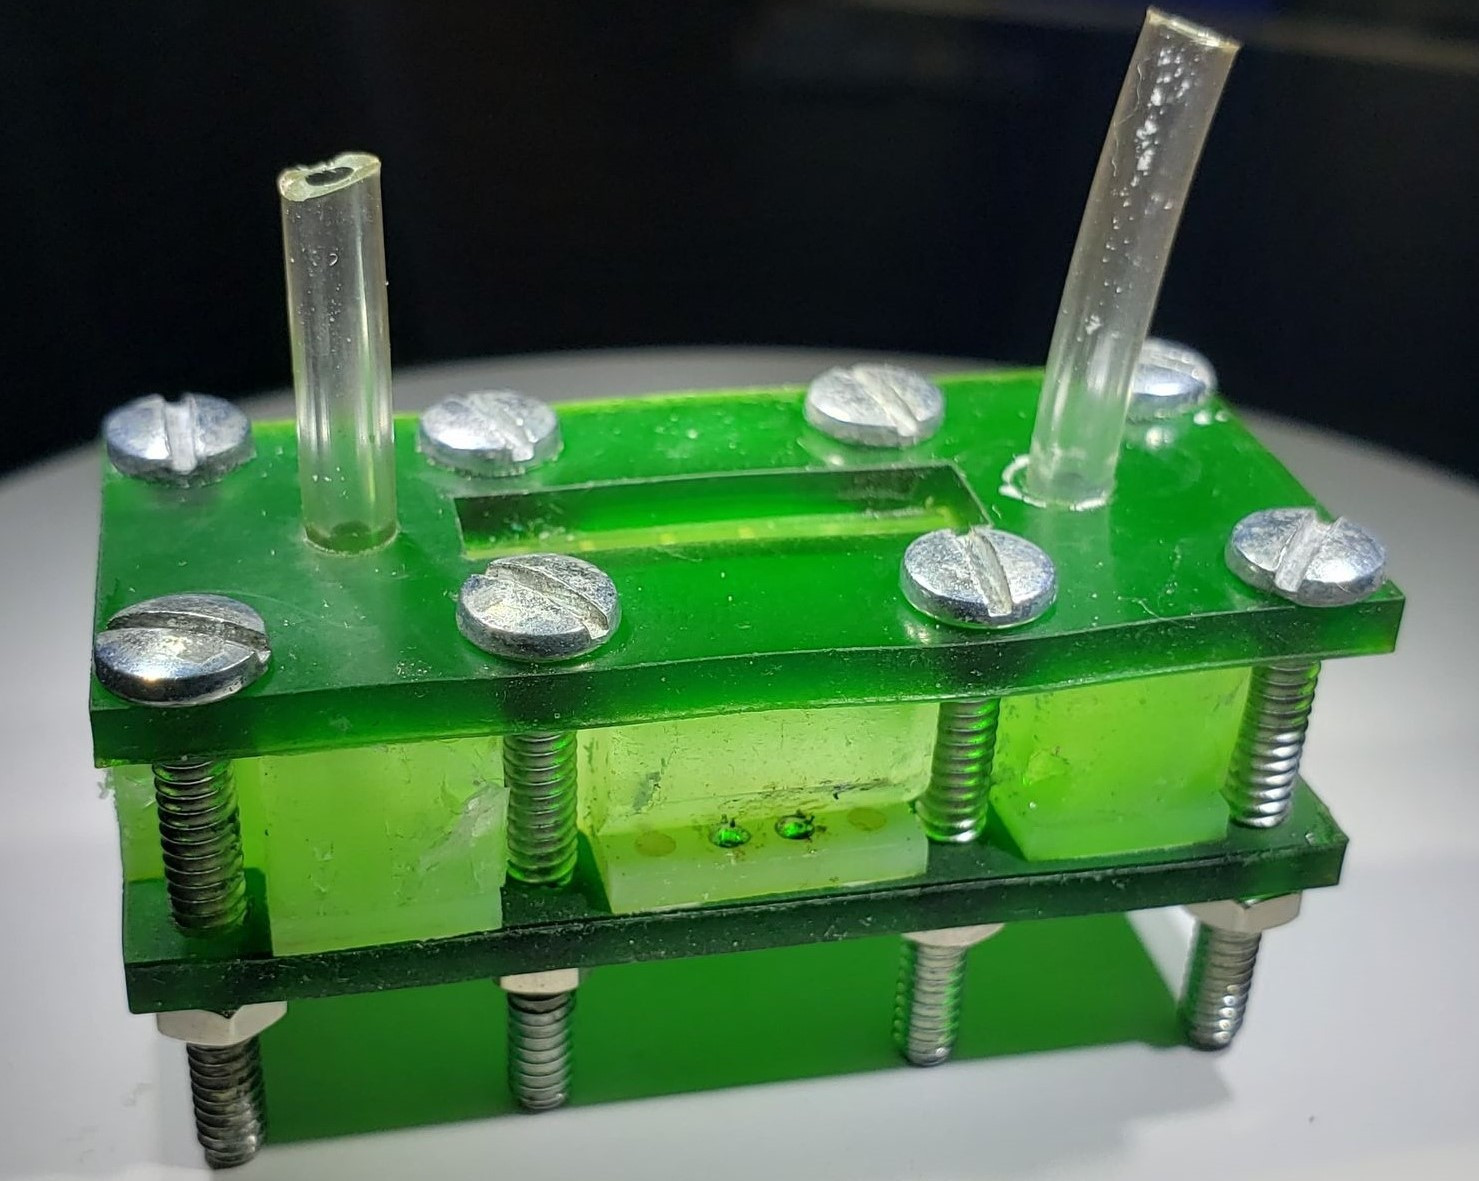
\includegraphics[width=0.6\textwidth]{MicrofluidicSystem}
    \caption{3d-printed microfluidic system used in this research to measure the impedance of a flowing liquid. It is composed of two 3d-printed squeezers, coplanar electrode pairs on PCB, a PDMS microchannel, soft tubes, and 8 screws and bolts.}
    \label{fig:MicrofluidicSystem}
\end{figure}
\begin{figure}[h]
    \centering
    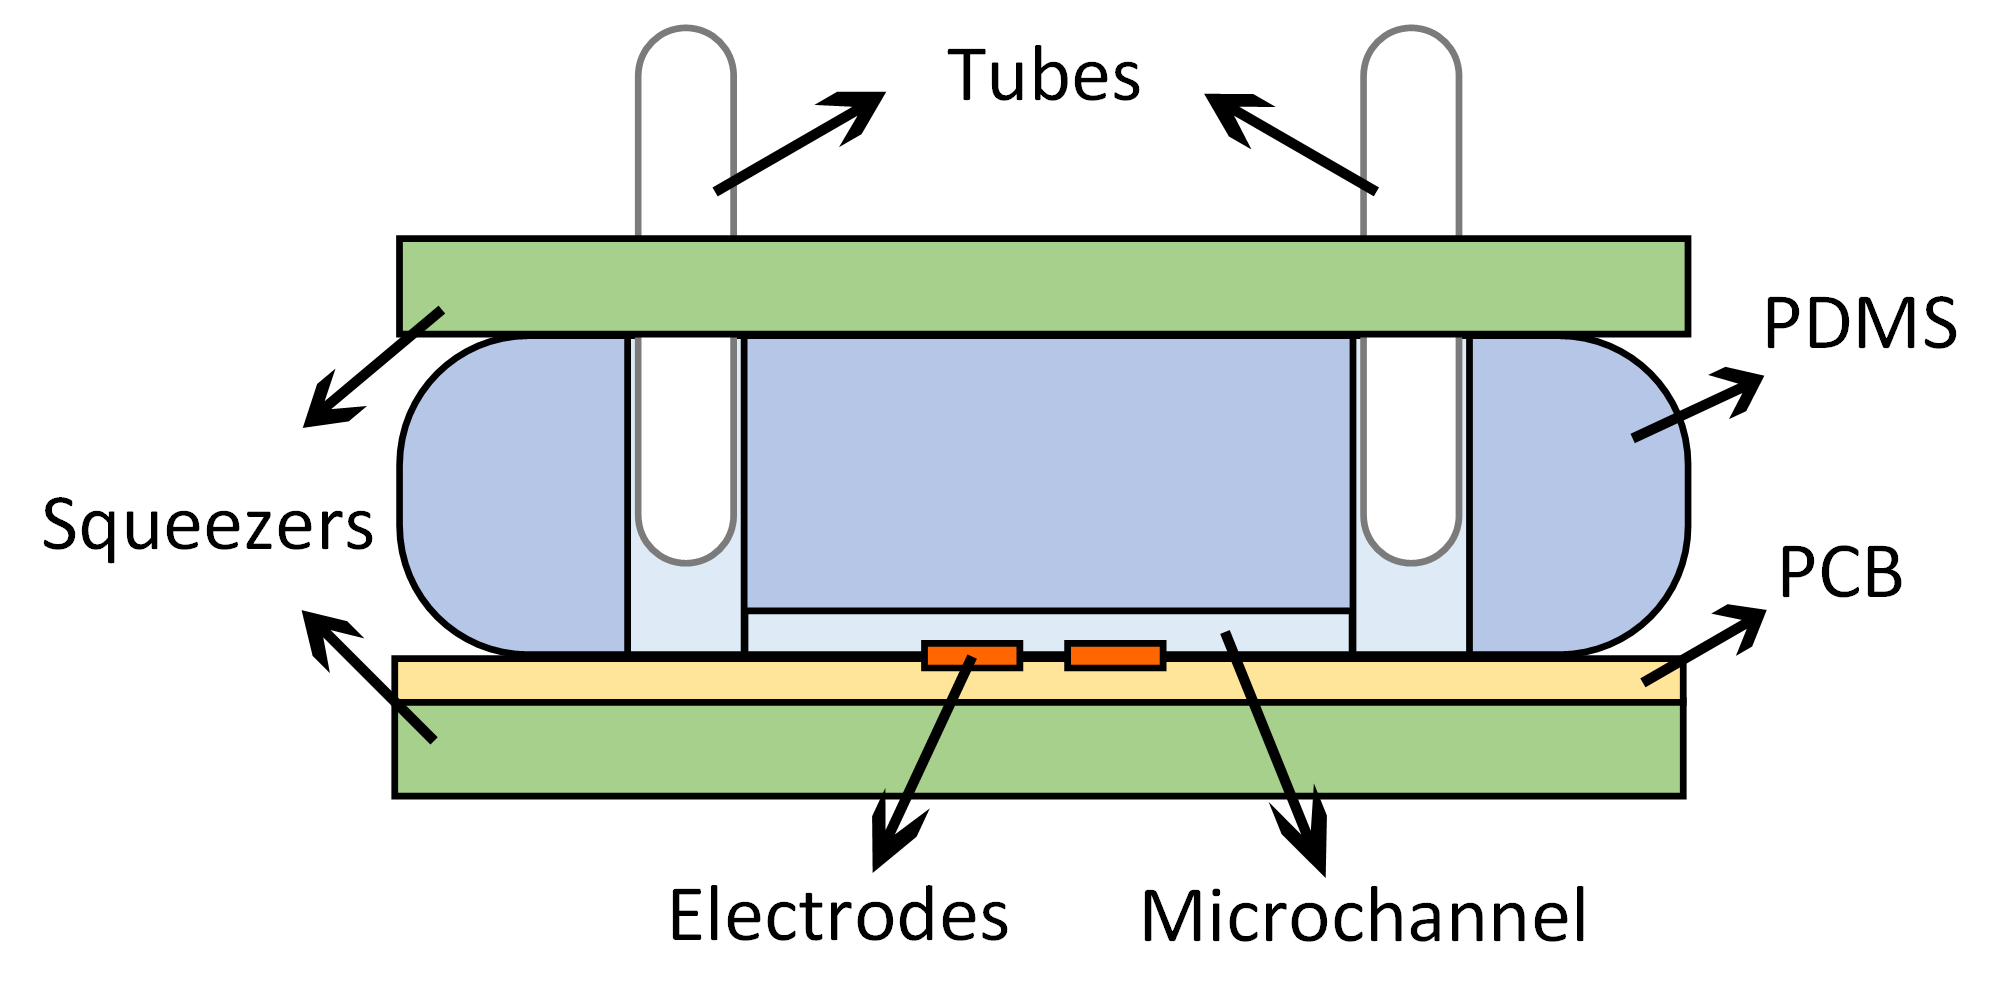
\includegraphics[width=0.9\textwidth]{DiagramMicrofluidicSystem}
    \caption{Diagram of the microfluidic system used in this research.}
    \label{fig:DiagramMicrofluidicSystem}
\end{figure}

The whole fabrication process is described in \autoref{fig:MicrofluidicsFabricationProcess}. A mold is initially realized on a CAD software such as Solidworks. This model is sent as a .STL file to the CADworks3D software to be meshed \cite{Cadworks3d}. This new meshed model is used in the software by the stereolithography 3d-printer CADworks3d H50-405 to print a 3d-mold using Master Mold for PDMS Device Photopolymer Resin \textsuperscript{TM} created by CADworks3D. The resin is then rinsed with IPA (90\%) or Methyl Hydrate for 5min and blow dried using an air gun. The mold is then cured using violet light in a LED light curing box machine (produced by Cadworks3d) sending wavelengths of 400nm for about 50min. PDMS (SYLGARD\textsuperscript{TM} 184 Silicone Elastomer Base) and a curing agent (SYLGARD\textsuperscript{TM} 184 Silicone Elastomer Curing Agent) are mixed at a ratio of 10:1 and degassed by letting the solution rest for 60min [48]. The mixture is put in the mold and cooked on a hot plate for 50min at 70° and dried overnight at 40° \cite{Trantidou2017}. A scalpel is used to gently prick-off the channel from the mold. The surfaces of the PDMS microchannel are exposed to plasma at 600 KPa for 1min. PEG is immediately put on the surface to keep its hydrophilicity for long periods of times. After waiting 10min, the PDMS microchannel is cooked 10min at 130° on a hot plate \cite{Trantidou2017}. A dry gun is blown on the channel to take away any residues. The PCB electrodes are aligned on the microchannel and a pressure is applied to seal them. Two 3d-printed squeezers are aligned at the top and bottom of the closed microchannel and screws are fitted to squeeze the PCB electrodes and PDMS microchannel in between the two squeezers. Finally, tubes are inserted at the inlet and outlet of the PDMS microchannel, concluding on the whole process. The microfluidic system is thus hermetic and easy to interact with. \par 
\begin{figure}[h]
    \centering
    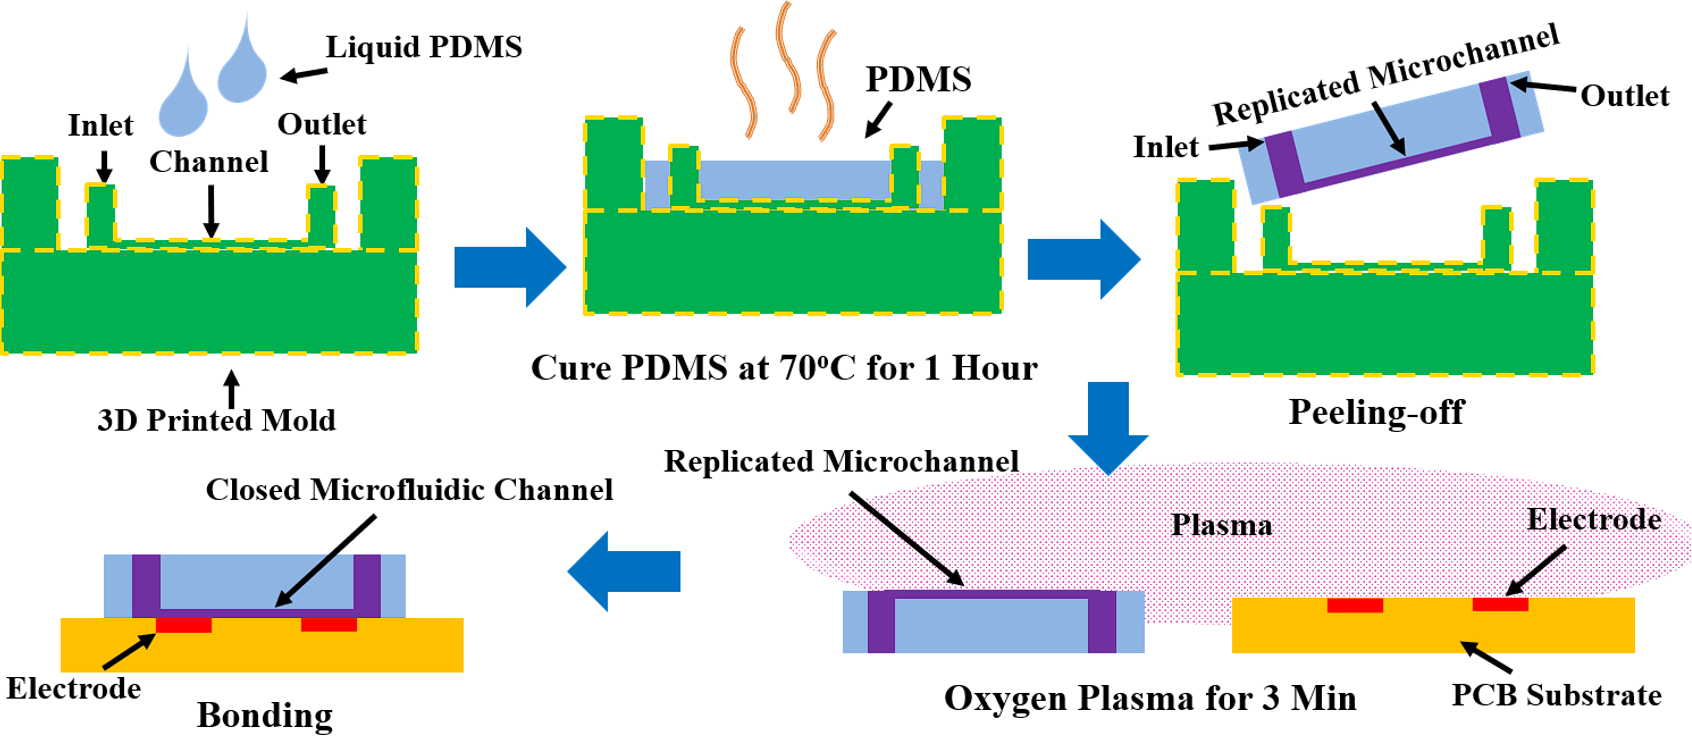
\includegraphics[width=0.99\textwidth]{MicrofluidicsFabricationProcess}
    \caption{Schematized steps for the fabrication process of the microfluidics system.}
    \label{fig:MicrofluidicsFabricationProcess}
\end{figure}

The shape of the mold is shown in \autoref{fig:3dprintedcomponents}. Using the H50-405, a theoretical resolution of 30 $\mu$m is possible, altough in practice, the minimum size of a channel possible to print without major defects is 90 $\mu$m. The PDMS cured in this mold solidifies into a structure with four openings in which the screws can be placed, as shown in \autoref{fig:PDMSChannel}. The electrode and squeezers share the same shape, as shown \autoref{fig:PCBElectrode2}.
%Scanning Electron Microscope (SEM) images were also taken to characterize the surface of the PDMS microchannel, as shown in \autoref{fig:SEMPDMS}
\begin{figure}[h]
\centering
%\begin{subfigure}{0.99\textwidth}
%\centering
    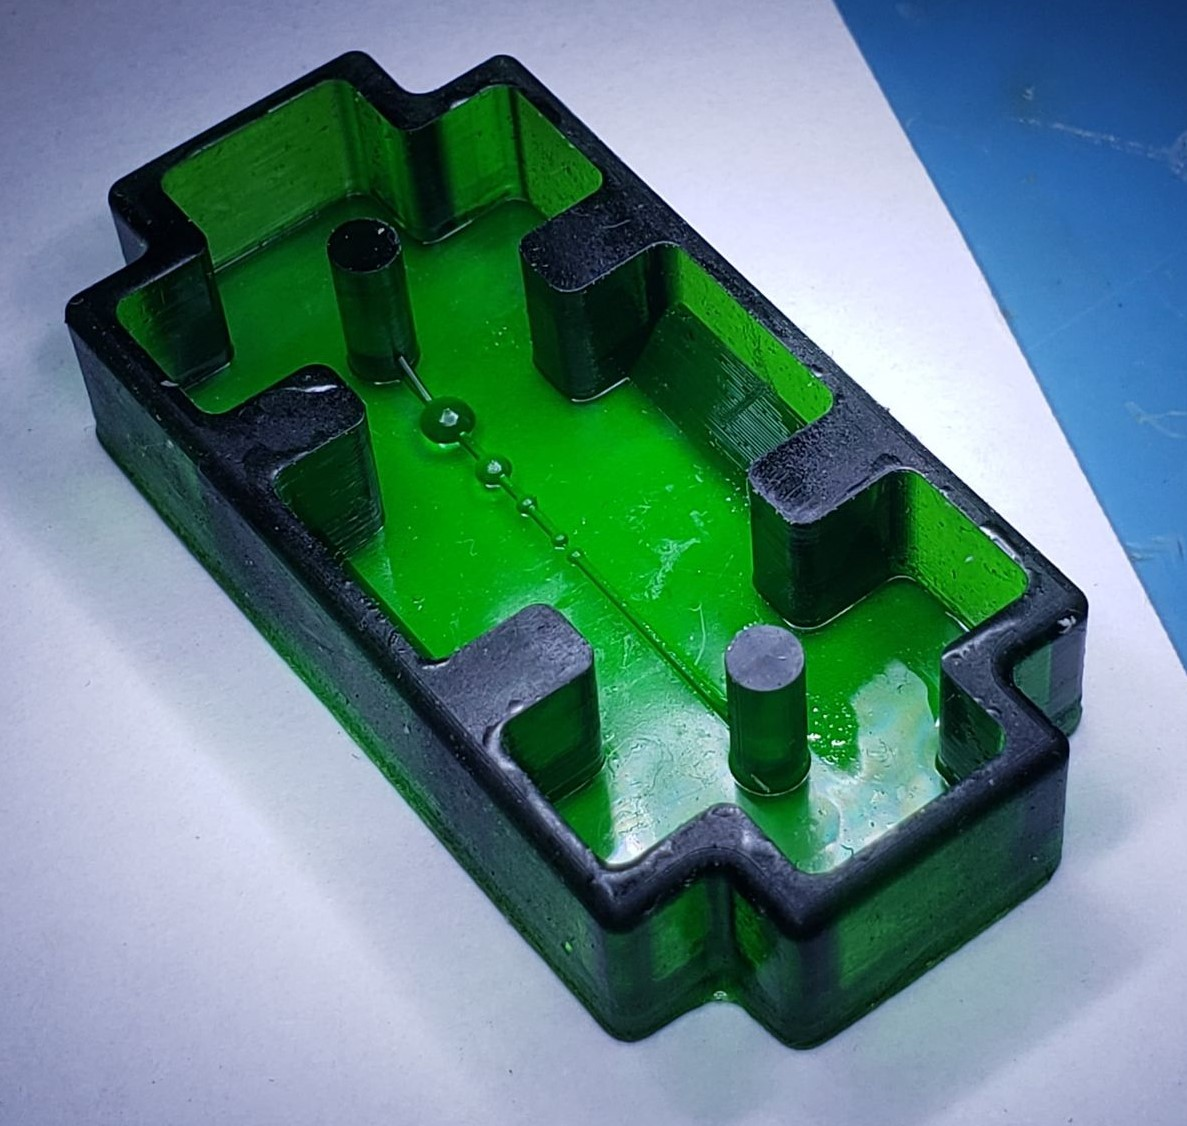
\includegraphics[width=0.8\linewidth]{Mold}
    %\caption{Mold.}
    %\label{fig:Mold}
%\end{subfigure}
%\begin{subfigure}{0.49\textwidth}
%\centering
%    \includegraphics[width=0.99\linewidth]{Squeezers}
%    \caption{Squeezers.}
%    \label{fig:Squeezers}
%\end{subfigure}
\caption{3d-printed mold of the microfluidic system.}
\label{fig:3dprintedcomponents}
\end{figure}

\begin{figure}[h]
\centering
\begin{subfigure}{0.49\textwidth}
\centering
    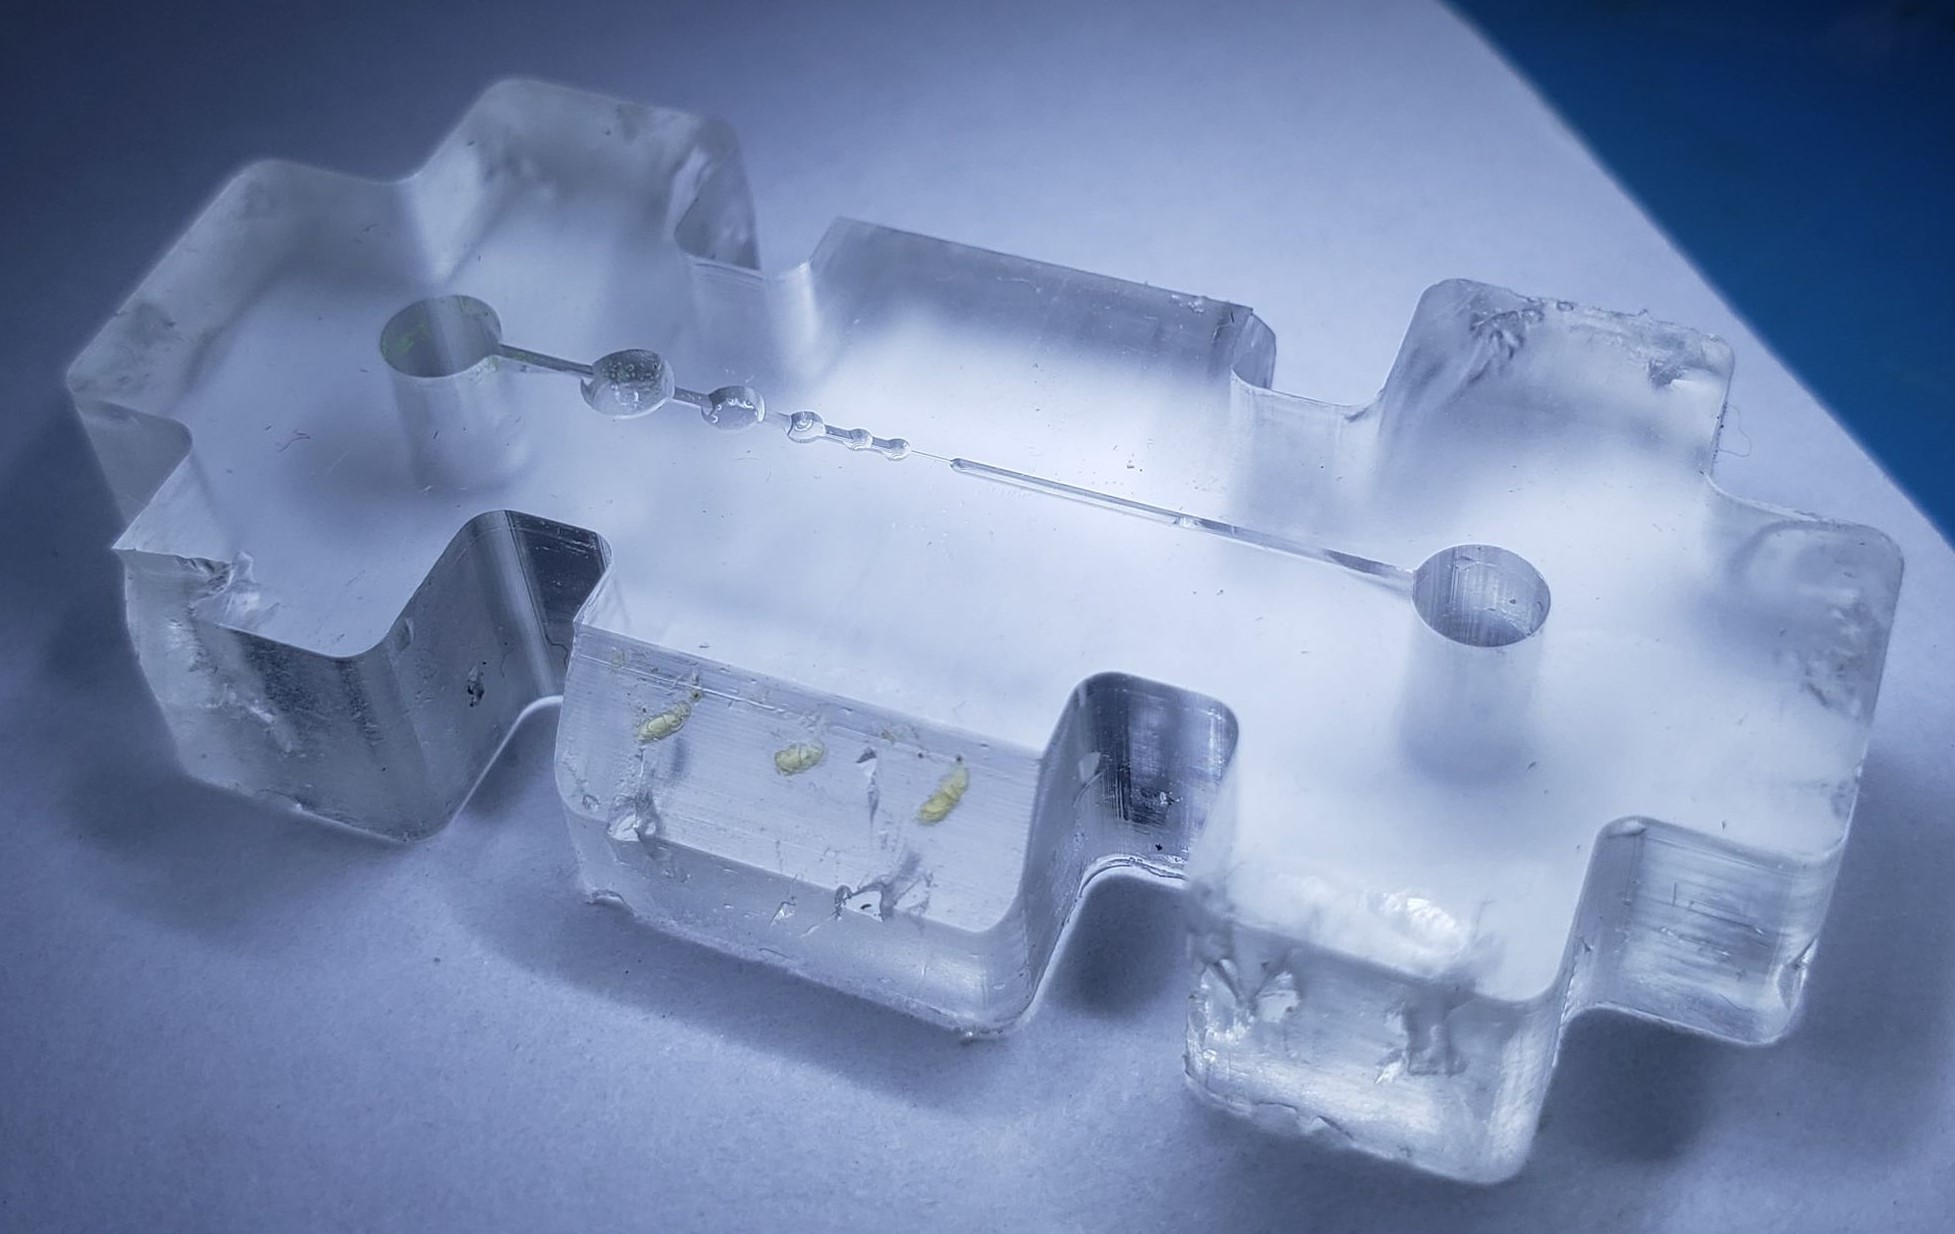
\includegraphics[width=0.88\linewidth]{FullChannel}
    \caption{Full view.}
    \label{fig:FullChannel}
\end{subfigure}
\begin{subfigure}{0.49\textwidth}
\centering
    \includegraphics[width=0.99\linewidth]{ZoomedChannel}
    \caption{Zoomed view.}
    \label{fig:ZoomedChannel}
\end{subfigure}
\caption{Solidified PDMS microchannel cured in the 3d-printed mold.}
\label{fig:PDMSChannel}
\end{figure}

%\begin{figure}[h]
%    \centering
%    \includegraphics[width=0.7\textwidth]{SEMPDMS}
%    \caption{SEM images of the surface of the PDMS microchannel. }
%    \label{fig:SEMPDMS}
%\end{figure}

The electrodes are fabricated on a one-layer PCB and were fabricated by PCBWay. They have a size of 46 $\times$ 21 $\times$ 1.6 mm. They are constructed from the conventional substrate FR-4 TG130 with smaller spacings of 4mils in the exact shape of the microfluidic channel so that they both might be fitted on top of one another. Finally, the surface finish is immersion gold (ENIG) (1U") with 1oz copper. These electrodes are 101.6 $\mu m$ wide and are separated by 101.6$\mu m$. Refer to \autoref{sec:ElectrodeDesign} for additional information on electrode-design. \par
\begin{figure}[h]
\centering
\begin{subfigure}{0.49\textwidth}
\centering
    \includegraphics[width=0.99\linewidth]{PCBElectrode2}
    \caption{Full view.}
    \label{fig:PCBElectrode2}
\end{subfigure}
\begin{subfigure}{0.49\textwidth}
\centering
    \includegraphics[width=0.7\linewidth]{PCBElectrode1}
    \caption{Zoomed view.}
    \label{fig:PCBElectrode1}
\end{subfigure}
\caption{3d-model of the electrodes on PCB as represented in Altium Designer.}
\label{fig:AltiumPCBElectrode}
\end{figure}

The 5-electrode configuration described in \citep{De_Ninno2017} has been chosen for this study. It creates a pattern in the observed signal that can be used to estimate the position of the cell in the channel. This is obtained at the price of a reduction in sensibility since the electrodes are further spaced apart from one another when arranged such. The 3d-model of the PCB electrode model, as represented in Altium Designer, is shown in \autoref{fig:AltiumPCBElectrode}, and the actual PCB electrodes are shown in \autoref{fig:PCBElectrode}. The aligment between the microchannel and electrodes is shown in \autoref{fig:AlignedElectrode}.

\begin{figure}[h]
\centering
\begin{subfigure}{0.49\textwidth}
\centering
    \includegraphics[width=0.96\linewidth]{PCBElectrode3}
    \caption{Full view.}
    \label{fig:PCBElectrode3}
\end{subfigure}
\begin{subfigure}{0.49\textwidth}
\centering
    \includegraphics[width=0.9\linewidth]{PCBElectrode4}
    \caption{Zoomed view.}
    \label{fig:PCBElectrode4}
\end{subfigure}
\caption{Practical electrodes on PCB.}
\label{fig:PCBElectrode}
\end{figure}

\begin{figure}[h]
    \centering
    \includegraphics[width=0.99\textwidth]{AlignedElectrode}
    \caption{PDMS microchannel alligned with the electrodes. }
    \label{fig:AlignedElectrode}
\end{figure}

\chapter{Measurement results}
The impedance spectroscopy of discrete resistors and capacitors forming complex systems will be measured in this chapter. Tests on saline water, as well as results in time with microbeads will be realized. Finally, the performances of the system will be discussed. 
\section{Discrete electrical measurements}
\label{sec:DiscreteResults}
\subsection{Discrete resistor}
The first results obtained using the impedance-sensing system is of an impedance spectroscopy for a 10 k$\Omega$ discrete resistor. Measured with an ohmmeter, its DC resistance is of 9.95 k$\Omega$. The impedance-sensing system is activated in Multi-frequency mode for a lowest excitation frequency of 20 kHz and a highest of 11.81 MHz (see \autoref{sec:MCUprocesses}). The square excitation signal is initialized at the lowest frequency, samples 64 data points, then the frequency is incremented logarithmally until the end frequency is reached. When that is the case, the frequency is reinitialized to the lowest frequency, and the process begins anew. The sampled data at the ADCs is represented in \autoref{fig:ResistorSignalsTime}, and were recorder for about 34 s at a sampling rate of 655 Sps, which is about five full spectroscopy cyclings. \par
\begin{figure}[h]
\centering
\begin{subfigure}{0.99\textwidth}
\centering
    \includegraphics[width=0.7\linewidth]{ResistorReal2}
    \caption{Real component.}
    \label{fig:ResistorReal2}
\end{subfigure}
\begin{subfigure}{0.99\textwidth}
\centering
    \includegraphics[width=0.7\linewidth]{ResistorImaginary2}
    \caption{Imaginary component.}
    \label{fig:ResistorImaginary2}
\end{subfigure}
\caption{Sampled signals in time at the ADCs, which represent the current response for the spectroscopy of a 9.95 k$\Omega$ discrete resistor.}
\label{fig:ResistorSignalsTime}
\end{figure}

The current responses of \autoref{fig:ResistorSignalsTime} are transformed into impedance magnitude and phase using \autoref{eq:CorrectedMagnitude} and \autoref{eq:CorrectedPhase}. All the impedance datapoints are represented as a function of frequency in \autoref{fig:ResistorImpedance}. \par
\begin{figure}[h]
\centering
\begin{subfigure}{0.99\textwidth}
\centering
    \includegraphics[width=0.9\linewidth]{ResistorMagnitude2}
    \caption{Magnitude.}
    \label{fig:ResistorMagnitude2}
\end{subfigure}
\begin{subfigure}{0.99\textwidth}
\centering
    \includegraphics[width=0.9\linewidth]{ResistorPhase2}
    \caption{Phase.}
    \label{fig:ResistorPhase2}
\end{subfigure}
\caption{Bode plot of the sampled impedance of a 9.95 k$\Omega$ discrete resistor with its theoretical value.}
\label{fig:ResistorImpedance}
\end{figure}

Some outliers can be observed from that dataset, which are introduced by a fault in the sampling protocol of the MCU. These errors are only present for the multi-frequency mode and will be kept to show the robustness of the measurements to outliers. \par

The values for low frequency also present a large imprecision. This imprecision is to be expected since the impedance-sensing system is definded only for frequencies above 100kHz. The LPF of the PSDs thus have a -3dB low-pass frequency of 20kHz, which does not totally attenuates the signal up until at least 70 kHz. \par

A significant bias can be observed at high frequency, which orgininates from a couple of causes. Firstly, the op-amps used in the electronics of the numerous modules (see \autoref{chap:Electronics}) have a frequency limit defined by their slew-rates, input capacitance, and gain-bandwidth. Secondly, capacitive coupling is introduced because of the PCB dielectric, traces, and wires. Those tend to attenuate the high-frequency components of signals. Since square excitation signals are used, the harmonics at higher frequencies get attenuated until the signal behaves much more like a sinewave around 20 MHz. As a result, the perceived impedance from the impedance-sensing device is increased since the measured current response gets lower at high frequency (refer to \autoref{eq:Magnitude}). \par

To solve this issue and linearize the sensor, a calibration is realized using resistors of different values. Since the parasitics are singular to the electronics, the same nonlinearity will be found for different values of resistance, which can be used as a frequency-dependant factor to linearize the magnitude and phase curves. The results of such a calibration are shown in \autoref{fig:ResistorImpedanceCalibrated}. \par
\begin{figure}[h]
\centering
\begin{subfigure}{0.99\textwidth}
\centering
    \includegraphics[width=0.9\linewidth]{ResistorMagnitudeCalibrated2}
    \caption{Magnitude.}
    \label{fig:ResistorMagnitudeCalibrated2}
\end{subfigure}
\begin{subfigure}{0.99\textwidth}
\centering
    \includegraphics[width=0.9\linewidth]{ResistorPhaseCalibrated2}
    \caption{Phase.}
    \label{fig:ResistorPhaseCalibrated2}
\end{subfigure}
\caption{Bode plot of the calibrated impedance of a 9.95 k$\Omega$ discrete resistor with its theoretical value.}
\label{fig:ResistorImpedanceCalibrated}
\end{figure}

Since this situation is only in the Real realm (no imaginary values are observed after calibration), the square to sine conversion is not needed, as proved in \autoref{sec:ImpedancePrinciples}. 

Thus, from the previous curves, errors of less than 1.5\% for the magnitude and of less than 2.5\% for the phase are observed for all the frequencies considered in the spectroscopy. The system thus works as intended. \par


\subsection{Complex discrete model}
The same procedure can be repeated for a more complex discrete model. A 10 k$\Omega$ resistor is placed in series with the parallel combination of a 4.47 k$\Omega$ resistor and a 100 pF capacitor. The current response at the ADCs are transformed into impedance magnitude and phase using \autoref{eq:CorrectedMagnitude} and \autoref{eq:CorrectedPhase}, then calibrated the same way as for the discrete resistor of the last example. All the calibrated impedance datapoints are represented as a function of frequency in \autoref{fig:RCImpedanceCalibrated}. \par

The impedance curves are calibrated to get \autoref{fig:RCImpedanceCalibrated}. \par
\begin{figure}[h]
\centering
\begin{subfigure}{0.99\textwidth}
\centering
    \includegraphics[width=0.9\linewidth]{RCMagnitudeCalibrated2}
    \caption{Magnitude.}
    \label{fig:RCMagnitudeCalibrated2}
\end{subfigure}
\begin{subfigure}{0.99\textwidth}
\centering
    \includegraphics[width=0.9\linewidth]{RCPhaseCalibrated2}
    \caption{Phase.}
    \label{fig:RCPhaseCalibrated2}
\end{subfigure}
\caption{Bode plot of the calibrated impedance of a 10 k$\Omega$ discrete resistor in series with a parallel combination of a 4.47 k$\Omega$ resistor and a 100pF capacitor.}
\label{fig:RCImpedanceCalibrated}
\end{figure}

These follow adequately the theoretical curves, but a bias is still to be found. This bias can be solved using the square to sine conversion adapted from \citep{Subhan2019} and described in \autoref{sec:ImpedancePrinciples}. This conversion can not be used on such a large dataset as in \autoref{fig:ResistorImpedanceCalibrated}, only the median value of all the data taken at one frequency points will be considered henceforth to represent spectroscopy. The results of such a conversion are shown in \autoref{fig:RCImpedanceSine}. \par
\begin{figure}[h]
\centering
\begin{subfigure}{0.99\textwidth}
\centering
    \includegraphics[width=0.9\linewidth]{RCMagnitudeSine2}
    \caption{Magnitude.}
    \label{fig:RCSineMagnitude2}
\end{subfigure}
\begin{subfigure}{0.99\textwidth}
\centering
    \includegraphics[width=0.9\linewidth]{RCPhaseSine2}
    \caption{Phase.}
    \label{fig:RCPhaseSine2}
\end{subfigure}
\caption{Bode plot of the calibrated impedance of a 10 k$\Omega$ discrete resistor in series with a parallel combination of a 4.47 k$\Omega$ resistor and a 100pF capacitor, after conversion from square to sine spectroscopy.}
\label{fig:RCImpedanceSine}
\end{figure}
At high frequencies, the square to sine conversion does not have enough datapoints to adequately do the conversion. This introduces a bias at high frequency. A way to solve this issue would be to extrapolate the behavior of the system from the previous points and use that extrapolation in the sqaure to sine conversion. For the case of simplicity in this study, no such correction shall be attempted.  \par

Apart from that, errors of less than 1.5\% for the magnitude and of less than 2.5\% for the phase are observed for all the frequencies considered in the spectroscopy. The system thus works as intended. \par
\section{Saline water measurements}
Now that discrete components were analyzed, the impedance is expected to be accurate for the following tests. It is then possible to measure the impedance of a complex system: saline water. A solution of saline water at 22 $^{\circ}$C is passed in a 180 $\mu m$ wide PDMS microchannel in the microfluidic system presented in \autoref{sec:PracticalMicrofluidic}, and the impedance spectroscopy is measured the same way as was done in \autoref{sec:DiscreteResults}. The calibrated and converted impedance curves are obtained and shown in \autoref{fig:SalineImpedanceSine}. \par
\begin{figure}[h]
\centering
\begin{subfigure}{0.99\textwidth}
\centering
    \includegraphics[width=0.9\linewidth]{SalineMagnitudeSine2}
    \caption{Magnitude.}
    \label{fig:SalineSineMagnitude2}
\end{subfigure}
\begin{subfigure}{0.99\textwidth}
\centering
    \includegraphics[width=0.9\linewidth]{SalinePhaseSine2}
    \caption{Phase.}
    \label{fig:SalinePhaseSine2}
\end{subfigure}
\caption{Bode plot of the calibrated impedance of a saline solution at 22 $^{\circ}$C containing 15g of salt for 100g of deionized water, after conversion from square to sine spectroscopy, measured by the two pairs of electrodes.}
\label{fig:SalineImpedanceSine}
\end{figure}

It is possible to see from \autoref{fig:SalineImpedanceSine} just how similar the responses of the two electrode pairs are. This proves the efficiency of the calibration step. The curves adequately represents some kind of a series capacitor and resistor, as was represented before in \autoref{fig:EIS_simplemodel}. 
\section{Microbeads measurements}
\label{sec:BeadsResults}
In order to replicate more accurately the expected behavior from cells and microparticles, Polystyrene microbeads are added to the 15\% saline solution. This SUT at 22 $^{\circ}$C is then passed in a 180 $\mu m$ wide microchannel and the impedance is measured for the single square excitation frequency of 1 MHz just as before. The sampling rate is set to a variable burst rate of 5.461 kSps and low-frequency constant rate of 30Hz to not overload the CPU (see \autoref{sec:MCU}). This means that the impedance is measured at fixed low-frequency of 30Hz until a significant difference is observed in the real components of any of the two electrode pairs. When such a difference is observed, a burst of 16 measurement points will be sampled at once at a frequency of 5.461 kSps. This method produces regularly fixed datapoint and dense bursts of data when a particle is detected. The raw signals obtained in this way are shown in \autoref{fig:BeadsADCResponse}. \par
\begin{figure}[h]
\centering
\begin{subfigure}{0.49\textwidth}
\centering
    \includegraphics[width=0.99\linewidth]{BeadsReal1}
    \caption{Real response of the first electrode pair.}
    \label{fig:BeadsReal1}
\end{subfigure}
\begin{subfigure}{0.49\textwidth}
\centering
    \includegraphics[width=0.99\linewidth]{BeadsReal2}
    \caption{Real response of the second electrode pair.}
    \label{fig:BeadsReal2}
\end{subfigure}
\vskip\baselineskip
\centering
\begin{subfigure}{0.49\textwidth}
\centering
    \includegraphics[width=0.99\linewidth]{BeadsImaginary1}
    \caption{Imaginary response of the first electrode pair.}
    \label{fig:BeadsImaginary1}
\end{subfigure}
\begin{subfigure}{0.49\textwidth}
\centering
    \includegraphics[width=0.99\linewidth]{BeadsImaginary2}
    \caption{Imaginary response of the second electrode pair.}
    \label{fig:BeadsImaginary2}
\end{subfigure}
\caption{Raw signals obtained at the ADCs of the impedance sensing system for saline water at 22 $^{\circ}$C mixed with Polystyrene microbeads of sizes between 10 and 90 $\mu m$  excited by a square excitation signal of frequency 1MHz in a 180 $\mu m$ wide microchannel.}
\label{fig:BeadsADCResponse}
\end{figure}

Let's numerically process the impedance magnitude and phase so that they become easier to analyze. Firstly, the mean values of the magnitude and phase of the two electrode pairs are taken out using wavelet decomposition. The signal is then de-noised, low-pass filtered, and smoothed so that the impedance spikes due to the particles are easier to recognize. The difference between the two electrode pairs are finally calculated since the object of interest in IFC is the amplitude difference and widths of the half-sine created by the impedance difference of the particle passing between two electrode pairs. The full signals are shown in \autoref{fig:BeadsImpedanceDifference}. \par
\begin{figure}[h]
\centering
\begin{subfigure}{0.99\textwidth}
\centering
    \includegraphics[width=0.99\linewidth]{BeadsMagnitudeDifference}
    \caption{Magnitude difference of the two electrode pairs.}
    \label{fig:BeadsMagnitudeDifference}
\end{subfigure}
\begin{subfigure}{0.99\textwidth}
\centering
    \includegraphics[width=0.99\linewidth]{BeadsPhaseDifference}
    \caption{Phase difference of the two electrode pairs.}
    \label{fig:BeadsPhaseDifference}
\end{subfigure}
\caption{Filtered impedance difference between the two electrode pairs measured as a function of time for saline water at 22 $^{\circ}$C mixed with Polystyrene microbeads of sizes between 10 and 90 $\mu m$  excited by a square excitation signal of frequency 1MHz in a 180 $\mu m$ wide microchannel. Different behaviors are observed at different timestamps of the signal.}
\label{fig:BeadsImpedanceDifference}
\end{figure}

Now, what exactly is happening with the electrode and solution to produce such curves? In the 82 seconds of the measurements, a couple of things happenned in the channel:
\begin{enumerate}
  \item The electrodes are initially relatively dry, meaning that the channel may have a residual liquid in it but the electrodes are not in full contact with it. This case-situation is associated to high values of impedance compared to the the impedance of the solution and is associated with a high variability of the measured impedance since the impedance measured on the electrodes is quickly modified by the shape and position of the residual liquid droplets that are found on the electrodes. This first situation is shown in \autoref{fig:BeadsImpedanceDifference5s}.
  \item The SUT then flows in the channel at a high speed. At this stage, between 5s and 10s, microparticles are flowing at such a high flow-rate in the channel that only 2 or 3 points are recorded when a particle passes in the channel. In other words, the sampling frequency is not high enough to accomodate such high flow velocity that only two or three samples are taken between the moment the particle arrives at the electrode pair and the moment it passed it. This behavior is shown in \autoref{fig:BeadsMagnitudeDifferenceZoomed10s}. Beads passed in the channel and the full-sine patterns are observed for six of them. 
  \item From the 10th to the 20th second, the liquid flow was stopped so that no beads would pass the electrodes. It is possible to see in \autoref{fig:BeadsImpedanceDifference20s} that no full-sine waves are observed in the impedance magnitude signal. 
  \item From the 22th to the 32th second, the liquid flow is resumed, at a more reasonable flow velocity this time. Full-sine waves with adequate numbers of samples are obtained, as shown in \autoref{fig:BeadsImpedanceDifference30s}. The beads generally produce impedance differences of less than 800 $\Omega$.
  \item From the 33th to the 38th second, air bubbles are introduced in the channel. These bubbles create massive impedance differences which are fairly easy to differentiate from the beads, as shown in \autoref{fig:BeadsImpedanceDifference38s}. The detection algorithm will discriminate between them later on. 
  \item From the 40th to the 63th seconds, particles flow in the channel at decent variable flow-rate. Some great particle recognition are observes, such as the ones in \autoref{fig:BeadsGreatDetection}. 
  \item After that, the liquid is flow is stopped for a moment, and the liquid is then flown out of the channel. A behavior similar to the beginning is observed, when the electrodes were only partially in contact with the SUT. 
\end{enumerate}

\begin{figure}[h]
\centering
\begin{subfigure}{0.99\textwidth}
\centering
    \includegraphics[width=0.9\linewidth]{BeadsMagnitudeDifference5s}
    \caption{Magnitude difference of the two electrode pairs.}
    \label{fig:BeadsMagnitudeDifference5s}
\end{subfigure}
\begin{subfigure}{0.99\textwidth}
\centering
    \includegraphics[width=0.9\linewidth]{BeadsPhaseDifference5s}
    \caption{Phase difference of the two electrode pairs.}
    \label{fig:BeadsPhaseDifference5s}
\end{subfigure}
\caption{[0s to 6s] A region of partially wet electrodes and air bubbles observed from the filtered impedance difference between the two electrode pairs obtained from the SUT.}
\label{fig:BeadsImpedanceDifference5s}
\end{figure}

\begin{figure}[h]
\centering
\begin{subfigure}{0.99\textwidth}
\centering
    \includegraphics[width=0.99\linewidth]{BeadsMagnitudeDifference10s}
    \caption{Full signal.}
    \label{fig:BeadsMagnitudeDifference10s}
\end{subfigure}
\begin{subfigure}{0.99\textwidth}
\centering
    \includegraphics[width=0.99\linewidth]{BeadsMagnitudeDifferenceZoomed10s}
    \caption{Signal zoomed on the patterns created by 6 beads.}
    \label{fig:BeadsMagnitudeDifferenceZoomed10s}
\end{subfigure}
\caption{[5s to 10s] A region of high flow velocity with beads observed from the filtered impedance magnitude difference between the two electrode pairs obtained from the SUT. Not many samples are taken for each particle since they flow too quickly.}
\label{fig:BeadsImpedanceDifference10s}
\end{figure}

\begin{figure}[h]
\centering
\includegraphics[width=0.99\linewidth]{BeadsMagnitudeDifference20s}
\caption{[10s to 20s] A region of no flow nor bubbles observed from the filtered impedance magnitude difference between the two electrode pairs obtained from the SUT. The spikes represent the baseline level of noise.}
\label{fig:BeadsImpedanceDifference20s}
\end{figure}

\begin{figure}[h]
\centering
\begin{subfigure}{0.99\textwidth}
\centering
    \includegraphics[width=0.99\linewidth]{BeadsMagnitudeDifference30s}
    \caption{Full signal.}
    \label{fig:BeadsMagnitudeDifference30s}
\end{subfigure}
\begin{subfigure}{0.99\textwidth}
\centering
    \includegraphics[width=0.99\linewidth]{BeadsMagnitudeDifferenceZoomed30s}
    \caption{Signal zoomed on the patterns created by 6 beads.}
    \label{fig:BeadsMagnitudeDifferenceZoomed30s}
\end{subfigure}
\caption{[20s to 33s] Beads pattern observed from the filtered impedance magnitude difference between the two electrode pairs obtained from the SUT. This time the beads flow slowly and more datapoints are taken for one bead.}
\label{fig:BeadsImpedanceDifference30s}
\end{figure}

\begin{figure}[h]
\centering
\includegraphics[width=0.99\linewidth]{BeadsMagnitudeDifference38s}
\caption{[33s to 38s] Bubbles observed from the filtered impedance magnitude difference between the two electrode pairs obtained from the SUT. The magnitude difference created by bubbles is really high, making them easy to discriminate from the beads.}
\label{fig:BeadsImpedanceDifference38s}
\end{figure}

\begin{figure}[h]
\centering
\begin{subfigure}{0.49\textwidth}
\centering
    \includegraphics[width=0.99\linewidth]{BeadsGreatDetection1}
    \caption{Great pattern obtained from 1 beads.}
    \label{fig:BeadsGreatDetection1}
\end{subfigure}
\begin{subfigure}{0.49\textwidth}
\centering
    \includegraphics[width=0.99\linewidth]{BeadsGreatDetection2}
    \caption{Great patterns obtained from 2 beads.}
    \label{fig:BeadsGreatDetection2}
\end{subfigure}
\caption{Examples of great microbeads patterns obtained from the SUT.}
\label{fig:BeadsGreatDetection}
\end{figure}

A particle detection algorithm is used on this dataset to recover the positions of the peaks. A peak detection algorithm is first used, followed by a Weak Supervision approach  \cite{ratner2017snorkel} using Snorkel to discriminate between the peaks obtained from bubbles, from the peaks obtained from beads, from the outliers and irregular data. \autoref{fig:BeadsPeakDetection} show the dataset with the detected peaks for a couple of beads. \par
\begin{figure}[h]
\centering
\includegraphics[width=0.8\linewidth]{BeadsPeakDetection}
\caption{Detected peaks from the filtered impedance magnitude difference between the two electrode pairs obtained from the SUT.}
\label{fig:BeadsPeakDetection}
\end{figure}

With these peak locations, it is possible to recover the amplitude and widths of the patterns, which are used to estimate the microbeads velocity and sizes, as explained in \autoref{sec:IFC} with \autoref{eq:sizeEstimation} and \autoref{eq:VelocityEstimation}. As an example, the pattern of \autoref{fig:BeadsGreatDetection1} will be studied. It has a positive impedance magnitude difference of 510 $\Omega$ and a negative impedance magnitude of 490 $\Omega$. Its $G$ constant is not known at this moment, but will be estimated using Big Data in \autoref{sec:BigData} as $G=7$. This leads us to a diameter value of 70 $\mu$m, which is adequate considering that this peak was fairly important and that the beads are of sizes between 10 $\mu$m and 90 $\mu$m. To calculate the beads velocity, the time it took for the particle to pass the electrodes is measured. This time is found to be 2.2 $\mu$s. The distance the bead had to flow through in that time, which is the distance separating the electrode pairs is divided to that time to obtain the particle velocity. That distance is of 406 $\mu$m. This leads to a velocity of 0.185 m/s.
%\section{Cells measurements}
%\input{CellResults}
\section{Big data}
\label{sec:BigData}
The same process as described in \autoref{sec:BeadsResults} can be repeated for other dataset, and the all the beads diameter and velocity can be estimated. This leads us to the true potential of IFC sensors in biological studies: Big Data. Big Data harnesses the power of numerical computations to efficiently extract relevant informations from enormous datasets. It could be imagined that a team of biologists collect the impedance data of millions of cells and particles using the portable device described in this memoir, and extract the important informations of these cells using Machine Learning, and high-end signal processing. \par

As a small-scale example, 7 datasets similar to the one obtained in \autoref{sec:BeadsResults} were collected and passed into the peak detection and classification algorithm. 2238 beads were detected and their magnitude, diameters, and velocity in the channels were calculated. \autoref{fig:BigDataMagnitudes}, \autoref{fig:BigDataDiameters}, and \autoref{fig:BigDataVelocity} show the distribution of these parameters. It is possible to see that the beads of sizes below 50 $\mu$m were not detected, simply because the impedance-sensing system lacks sensibility to detect such small impedance variations. The discrete distribution for the velocities should also be noted, which is a direct result of the lack of sampling points to characterize some of the faster velocities, as explained before in \autoref{sec:BeadsResults}. 
\begin{figure}[h]
\centering
\includegraphics[width=0.99\linewidth]{BigDataMagnitudes}
\caption{Scattergram of the impedance magnitude measured by both electrode pair for the 2380 detected microbeads of sizes between 10 $\mu$m and 90 $\mu$m.}
\label{fig:BigDataMagnitudes}
\end{figure}

\begin{figure}[h]
\centering
\includegraphics[width=0.7\linewidth]{BigDataDiameters}
\caption{Histogram of the estimated diameters of the 2380 detected microbeads of sizes between 10 $\mu$m and 90 $\mu$m.}
\label{fig:BigDataDiameters}
\end{figure}

\begin{figure}[h]
\centering
\includegraphics[width=0.7\linewidth]{BigDataVelocity}
\caption{Histogram of the particle velocity of the 2380 detected microbeads of sizes between 10 $\mu$m and 90 $\mu$m.}
\label{fig:BigDataVelocity}
\end{figure}
\section{Performances}
The performances and characteristics of the impedance-sensing device and microfluidics system are summarized in \autoref{tab:Performances}.

\begin{table}[h]
\centering
\caption{\label{tab:Performances} Measured system performances}
\begin{tabular}{|c | c|} 
 \hline
 Parameter & Value \\ [0.5ex] 
 \hline
 Supply voltage (battery) & 2.5 V to 3 V  \\ 
 \hline
 Maximum power consumption & 1.75 W \\
 \hline
 Nominal power consumption & 1.25 W \\
 \hline
 Input voltage @ electrodes & 450 mV \\
 \hline
 Sampling frequency & 5461 Sps or 650 Sps \\ 
 \hline
 Excitation frequency range & 30 kHz to 15 MHz \\
 \hline
 Excitation frequency resolution & 100 Hz \\
 \hline
 Type of excitation signal & Square \\ 
 \hline
 Impedance magnitude range & 800 $\Omega$ to 50 k$\Omega$ \\
 \hline
 Impedance magnitude precision & < 3\% \\
 \hline
 Impedance phase precision & < 3\% \\
 \hline
 PCB size & 50 $\times$ 50 $\times$ 15 mm \\ [1ex] 
 \hline
 Microchannel size & 150 $\times$ 150 $\mu$m \\
 \hline
 Electrode width & 106 $\mu$m \\
 \hline
 Electrode separation & 424 $\mu$m \\
 \hline
\end{tabular}
\end{table}

The power consumption is adequate for a portable application. It could, however, be greatly reduced by transforming the PCB to an integrated application in a custom-made IC, considering that the vast majority of the power is dissipated in the op-amps, which serve to do only basic functions such as inverting and amplifying signals. This is something that will be explored in the next phases of the project. 

\chapter{Conclusion}
The portable impedance-sensing device described in this memoir, coupled with the microfluidics systems, are effectively capable of measuring and estimating the properties of the microparticles of sizes going as low as 50 $\mu$m. The system created for this MSc is novel, and the first found in the scientific literature to achieve such a sensitivity level while boasting a small size, low-cost, and low power-consumption. The impedance-sensing device takes 50 mm $\times$ 50 mm $\times$ 15 mm of space, while the microfluidics system takes 46 mm $\times$ 25 mm $\times$ 50 mm. The impedance-sensing system needs 1.5 W to function adequately, and is powered by a battery of a voltage between 2.5 V and 3 V. The impedance can be sampled for frequencies between 30 kHz and 15 MHz. The impedance spectroscopy of discrete resistors and complex discrete models were obtained and their impedance spectrum closely followed the predictions. The impedance profiles of saline solutions were also obtained, from which microbeads were added. The impedance of the solution with microbeads was analyzed in the microfluidic system and 2238 microbeads were detected. From that dataset, the important parameters of microbeads were found, which proved the usefulness of the biosensor as a portable device capable of measuring micron-scale particles. \par

The project could be improved in a couple of ways. (1) The electronic of the impedance-sensing system uses mostly discrete components such as op-amps to accomplish functions which would be better suited to integrated electronics. A custom-made IC would be perfect for this applications and could probably reduce the power-consumptions from 1.25 W down to a couple of mW. (2) Using a different 3D-printer, such as the one designed by \citep{Gong2017}, which achieved structures with minimal microchannel widths of 20 $\mu$m, would help increase the sensitivity of the particle detection. (3) The electronics of the impedance-sensing system and PCB fabrication could be improved to reduce the baseline noise values. (4) The ADCs ranges could be tuned to better fit the measured results, which would increase the ENOB in return.

%\chapter{Inserted article}
%Measured performances in a table. Cite Bouzid2022. 

% Format a LaTeX bibliography
\makebibliography
%\nocite{*} %Check if I want to cite all references or only those in the text

\appendix
\chapter{Capacitance biosensors}
\label{app:CapacitanceBiosensors}
This review of capacitance biosensors was features in Seyedeh Nazila Hosseini's "A Comprehensive Review of Advances in Electrochemical Biosensors for Microbial Monitoring" that will be published in a couple of months in 2022 for TBioCAS. \par

Capacitance-based biosensors comprise such measurement method built upon a measure of the capacitance of an analyte. Such techniques can be found in the scientific literature in a variety of forms. The most important ones concerning bacterial monitoring are: Charge Sharing capacitive sensors, Charge-Based capacitance measurement (CBCM) and Capacitance-to-Frequency Converter, which are all high resolution and compact solutions to measure capacitances. \par

The first technique relies upon the charge sharing principle. Two capacitors $C_{N1}$ and $C_{N2}$ with known values of capacitances are placed between DC tension nodes $V_{DD}$ and $V_{SS}$ and separated by three MOSFET switches M1, M2 and M3. This switched capacitance configuration creates two intermediate nodes N1 and N2 associated with respective nodal tension $V_{N1}$ and $V_{N2}$. The unknown capacitance is then placed at one of the nodes and the measurement is accomplished by two successive operations realized with the MOSFETs. Firstly, during what is called the reset phase, the switches M1 and M3 are turned on while M2 is kept blocking. This charges the capacitances at nodes N1 and N2 to $V_{DD}$ and $V_{SS}$ respectively. Then, during the evaluation phase, the switches M1 and M3 are shut while M2 is activated, which causes a redistribution of the charges accumulated in $C_{N1}$ and $C_{N2}$ that leads to a nodal tension which follows:
\begin{equation}
   V_{N}(t) = \frac{V_{DD} (C_{N1}+C_{sensed}) + C_{N2} V_{SS}}{C_{N1}+C_{N2}+C_{sensed}}
\end{equation}
The only unknown parameter becomes the sensed capacitance, which can then be deduced easily [1]:
\begin{equation}
   C_{sensed}(t) = \frac{(V_{DD}-V_{SS}) C_{N2} - (C_{N1}+C_{N2}) V_N}{V_N}
\end{equation}
This configuration can be integrated efficiently on sensing electrode to minimize die space and features a great linear high sensitivity dependence between the output voltage and the sensed capacitance. Compensation schemes for the Fixed-Noise Pattern (FNP) are also available in the literature to further increase the performances [2]. However, the use of switching capacitors is not free from drawbacks. Indeed, such circuits suffer from speed limitation caused by the time needed to fully charge and discharge the capacitances. They also necessitate two non-overlapping clock signals in order to function properly, otherwise charge injection and clock feed-through caused by the MOSFET switches would cause gain error, offset and distortion \cite{horowitz1989art}[3]. The inverse relation between $C_{sensed}$ and $V_N$ creates a limited range of measurable capacitance with an adequate precision [1]. \par

The second technique is Charge-Based Capacitance Measurement (CBCM) which permits, in its original version proposed in 1996 by J. C. Chen [4] a really high precision and sensitivity attaining attofarad resolution. The simplest version of this circuit is made of two switching MOSFETs M1 and M2 with a sensed capacitance Csensed in between them, both placed between the power supplies Vss and Vdd.  They are both excited by non-overlapping excitation signals, that successively charge and discharge the sensing capacitance. The non-overlapping signal is required to prevent short-circuiting the power-supplies. Supposing that the switches M1 and M2 are ideals and that the excitation frequency of the non-overlapping clock signals is low enough to allow a full charge and discharge of the sensed capacitance, the transient current $I_C$ in the switches becomes proportional to the frequency of the clock signal $f$, the reference tension $V_{DD}$ and the sensed capacitance $C_{sensed}$. In this situation, the form of the transient current is of no importance, only the average current value is used to obtain the sensed capacitance value [4]. The average current furnished by the power-supply then becomes the sum of the quiescent current and the transient current:
\begin{equation}
   I_{AVG} = \frac{I_{DC}}{2} + C_{sensed} V_{step} f
\end{equation}
By adding an integrator at $V_{DD}$ or $V_{SS}$ made with a capacitor of value $C$, it becomes possible to deduce the average current, which further allows the deduction of the sensed capacitance value [7][10]: 
\begin{equation}
   V_{out} = -V_{DD} - \frac{T}{C} I_{AVG}
\end{equation}
It has since then been significantly improved upon and applied notably for particles detection and bacteria monitoring. One of the first upgrades made upon this simple circuit was to add a CMOS current mirror at the power supply in order to replicate the current waveform of the charge and discharge of the sensed capacitance in another branch of the circuit, which could then be used for referential purposes for a differential measurement. Another improvement that can be realized on this circuit is to measure the average current for different voltage value of the power-supply $V_{DD}$: the slope of the best linear regression through the data obtained can be used to calculate a better sensed capacitance less affected by the parasitic capacitances present in the model [10]. On-board compensation schemes can also be added to directly eliminate the parasitics, at the cost of additional on-board die, power-consumption, and complexity \cite{horowitz1989art}[8]. \par

CBCM are effective capacitance sensors since they do not require elaborate circuits in order to attain adequate results. They do not, in comparison to voltammetry, amperometry and electrochemical impedance spectroscopy (EIS), require readout circuits or signal conditioning modules, which makes them incredibly compact and suitable for high-throughput applications where a low on-chip area is required [3]. The resolution limit is effectively caused by the mismatch between the drain junction and overlap capacitance of the transistors of the design [4]. The charging time of the capacitances can become extremely small for highly conductive electrolytes, which makes the sensitivity of this device the main point to optimize [2]. \par

The final technique uses a Current-to-Frequency Converter (CFC) to change a capacitance value to a frequency, which timings can be measured by any digital circuit that can count reference crossings. This approach generally combines a Current-To-Voltage Converter (CVC) and a Voltage-to-Frequency Converter (VFC) into one compact design to bypass the need for intermediate signal constituents. One such design can be accomplished with a simple differential design: a constant current is sent to a sensing capacitance and a reference electrode; the difference is calculated and the resulting waveform is integrated until a reference threshold is attained, at which point an output is produced and the input is reset; the output frequency thus depends on the capacitance difference between the electrodes [5]. Another way to accomplish a CFC is by devising a self-oscillating circuit in a closed-loop pattern based on an integrating amplifier and a comparator with set reference values, with an input current that oscillates based on its output. This way, the tension at the electrode is successively increased and decreased proportionally to its capacitance value, and a bit-stream at the comparator’s output is created that has a frequency dependent on the rate of change of the electrode:
\begin{equation}
   \frac{1}{f} = 2 R C * ln(\frac{1}{1-\frac{V_{ref}}{I_{ref} R}})
\end{equation}
Where $R$ and $C$ are the electrode-electrolyte interfacial parameters, $I_{ref}$ is the input current and $V_{ref}$ is the magnitude value of the voltage references for the comparator [6]. \par

The main advantage of CFC sensors is that they eliminate the need for an ADC circuit, which makes them cost and space-efficient [6]. They however suffer from a high FNP when miniaturized because no compensation schemes exist for them [11]. Additionally, the need for a comparator makes this configuration less optimal for highly integrated designs and high throughput application, such as Multi-Electrode Array (MEA) for spatial recognition of particles [2].\par

The main concern about capacitive measurement applied to bacteria measurement is that the sensed capacitances are generally extremely small, typically a few femtofarads, which means that the parasitic capacitances and noise cannot be neglected. Additionally, the capacitance conversion can be further troubled by the high conductivity of the bacterial medium. To achieve better precision and to reduce the effects of parasitic, a differential configuration is often used. This, however, is far from optimal for high-throughput application because each sensed capacitance must be linked to a similar valued reference capacitance, which reduces the versatility of the sensor for a broader range of applications considering that the fixed calibration resistance is calibrated for a given electrolyte [2]. Capacitance sensors also do not suffer from measurement drifts caused by long-time monitoring, which counters the need for a self-calibration module [9].\par
\chapter{Impedance Microbiology}
Impedance Microbiology (IM) \cite{stewart1899charges} is a laboratory-technique used by microbiologist to establish the microbial number density of a sample. Its founding principle is that the metabolism of microorganisms transforms uncharged or weakly charged compounds present in the growth medium (such as sugars and proteins/peptides) into highly charged ones (carbon dioxide, organic acids, hydrogen ions, etc.). By monitoring the electrical properties of the culture broth, it is then possible to infer in real time the changes happening in its bacterial concentration: the growth in number of the microbial population corresponds to an increase in the produced metabolites, thus in the medium’s conductivity \cite{Grossi2017,Kargupta2018,Xu2016}. Again, this technique only teaches about the bacterial population, and not the individual bacteria. \par

The growth phases of bacterial colonies generally follow three growth steps, which can be associated with the change in conductivity of the growth medium, as illustrated in \autoref{fig:GrowthPhase}. An initial lag phase, in which the bacteria prepare for duplication is characterized by a low constant conductivity; the log phase, when the bacterial growth is maximal, can be retraced when the bacterial concentration reaches the critical microbial concentration threshold $C_{TH}$; the stationary phase, when the bacteria have depleted the nutriments in the medium, can be deduced by the halt of the conductivity after the log phase; the dead phase follows when the bacteria dies per lack of nutriment, and is the only phase that cannot be deduced by the medium’s conductivity since the highly charged compounds that now occupies the medium do not vanish after the death of the bacteria. Information about the life cycle can be used to differentiate between bacterial population since these characteristics are unique to each specie \cite{Sylvain2018}. 
\begin{figure}[h]
    \centering
    \includegraphics[width=0.7\textwidth]{GrowthPhase}
    \caption{Growth phases of a bacterial population.\citep{wang2015bacterial}}
    \label{fig:GrowthPhase}
\end{figure}

The first step in IM is to add an aliquot of the substance of interest (blood, sputum, food, specific microbe, yeast, etc.) to a chosen culture broth, while maintaining external conditions at a constant level suitable for an optimum growth of the target microorganisms. From there, the microorganisms, if present in the sample, will metabolize the compounds of the culture broth, which will modify the properties of the medium, such as pH, O2/CO2 levels, and electrical conductivity \cite{Kargupta2018,Xu2016}. In IM, it is the electrical conductivity which is monitored regularly as a function of time, generally by measurements of the complex impedance of the sample. The measured conductivity starts at a low baseline value and suddenly increases after a critical microbial concentration threshold $C_{TH}$ (in the range of 106-107 cfu/ml for cells in suspensions \cite{Xu2016,Lei2014}) is reached, which depends on the type of bacteria, electrodes, and culture broth chosen for the test. Since bacteria replication through binary fission is completed in a fixed time, it is then possible to deduce the initial microbial concentration $C_0$ of a sample by noting the Detect Time ($DT$) needed to attain the critical microbial concentration that significantly increases the conductivity. Seeing that DT is a linear function of the logarithm of the initial concentration, that value can be easily deduced \cite{Grossi2009,Xu2016}:
\begin{equation}
DT = A \log(C_0) + B
\end{equation}
\begin{equation}
C_0 = 10^{\frac {DT-B}{A}}
\end{equation}
Here, $A$ and $B$ are parameters that vary accordingly to the type of bacteria and culture broth chosen for the experiment, as well as some environmental conditions such as pH and temperature. They can be deduced with a calibration using bacteria and broth with known initial concentration and $DT$ in a supervised environment, followed by an adequate linear regression \cite{stewart1899charges}. \par
\chapter{Impedance analyzer IC AD5933}
In practice, the best performances for measuring impedance are obtained by using discrete Integrated Chips (IC) \cite{horowitz1989art}. For example, a waveform generator using the ICs AD5930 or AD5932 could be used to send a known sinusoidal signal to the SUT, which would then be measured by an ADC linked to a microcontroller that calculates the unknown impedance’s modulus and phase \cite{grossi2019electrical,Chowdhury2017}. A suitable Analog Front End (AFE) would be placed between the waveform from the generator and the SUT to better suit the specific application. \par

The specialized impedance analyzer IC AD5933 \cite{AD5933-documentation} can be used in a likewise fashion. This IC combines in a small package a sinusoidal voltage generator made from a 27-bits phase accumulator Direct Digital Synthesis (DDS) core and a Digital-to-Analog Converter (DAC), a TIA with a programmable gain, a 12-bits 1 MSPS ADC with a 100 kHz antialiasing filter, and an onboard Digital Signal Processing (DSP) unit which calculates a 1024 points Discrete Fourier Transform (DFT) with a Multiplier Accumulator (MAC) \cite{horowitz1989art}. Its functionalized diagram is illustrated in \autoref{fig:AD5933_diagram}. After the calculations, it yields the 16-bits real and imaginary impedance components through an I2C communication protocol \cite{horowitz1989art}, which can then be used to deduce the magnitude and phase of the SUT’s impedance:
\begin{equation}
   \lvert Z \rvert = \sqrt{Re(Z)+Im(Z)}
\end{equation}
\begin{equation}
   \theta = atan(\frac{Im(Z)}{Re(Z)})
\end{equation}
\begin{figure}[h]
    \centering
    \includegraphics[width=1\textwidth]{AD5933_diagram}
    \caption{Functional bloc-diagram of the AD5933 IC \cite{AD5933-documentation}.}
    \label{fig:AD5933_diagram}
\end{figure}
As explained by \citep{Chabowski2015}, the AD5933 IC suffers from multiple inherent defects, which can mostly be accounted for by a careful design of the AFE. Firstly, a serial resistance exists at the output transmit stage, which limits the lower bound of impedance measurement. The addition of a buffer between the transmit stage and the SUT helps to reduce to a minimum this parasitic serial resistance. \par

Secondly, the ADC suffers from a dead zone which can affect the measurement for voltages at the ADC’s input lower than 15 mV. Adding multiple switchable resistances for the TIA’s feedback resistance can solve this problem and makes it so that the tension at the ADC is pushed further to increasingly high and increasingly low values of SUT’s impedance, hopefully outside of the bounds of the given application \cite{Chabowski2015,horowitz1989art}. See \autoref{sec:PGA}. \par

Thirdly, the transmit stage provides varying Direct Current (DC) bias which must be accounted for to not saturate the op-amps. This can be done with a DC canceller circuit \cite{horowitz1989art}. In its simplest form, only a High-Pass filter (HPF) would suffice, but this configuration suffers from long measurement time at low frequency. HPFs are generally made with resistors and capacitors in a RC filter, which suffer from a long settling time caused by the transitory state of the HPFs. Considering that “the time constant of the RC filter has to be significantly longer than the longest period of the excitation voltage”\cite{Chabowski2015} in order to obtain a decent precision, the settling time can become unsatisfactorily high for low excitation frequency \cite{horowitz1989art}. \citep{Chabowski2015} proposed a novel DC canceller based on a positive and negative peak detector to reduce the measurement time. This circuit has been chosen by the author (K.Bouzid,2022) to be used in the final design of the EcoChip2 in \citep{das2020ecochip}, and will be described later in \autoref{app:Ecochip}. \par

Fourthly, the DFT introduces discontinuities in the digital calculations that affect the impedance measurement. The AD5933 implements a single-point DFT, which means that the analysis frequency running inside the MAC core should be at the same frequency of that of the output excitation signal. A smooth transition between the period of the excitation signal of the SUT and the DDS generator signal is thus necessary to prevent this leakage. In other words, the sample time of the DFT must be an integer $k$ factor of the DDS generator clock, otherwise numerical approximations will diminish the precision of the data. To that end, the DFT sample time and DDS period should follow the following equality \cite{Chabowski2015}:
\begin{equation}
   T_s = 1024 \frac{16}{MCLK} = k T_{DDS} = k \frac{2^{27}}{DDS \frac{MCLK}{4}}
\end{equation}
Where $MCLK$ is the master clock frequency, which is at the same frequency of the MAC unit; and $DDS$ is the DDS tuning word set on 27 bits and used to set up the excitation frequency. \autoref{fig:AD5933_leak} illustrates the impact of the leakage on the normalized impedance measured for different value of the factor $k$. It also shows that for values of $k$ superior to 10, the error is practically null, and integer values for this coefficient are no longer necessary. However, for higher value of $k$, another problem appears. The high value of the DDS tuning word causes the output of the DAC to change too much at each clock cycle, which results in a stair-shaped excitation signal that appears digitized. This distortion distorts the measurement made by the DFT, which corrupts the impedance measurement. Considering these matters for the DFT, a tunable MCLK should be provided with the design, to obtain $k$ values in the range 10 to 100 for all frequencies of the desired impedance frequency spectrum. \cite{Chabowski2015} \par
\begin{figure}[h]
    \centering
    \includegraphics[width=0.7\textwidth]{AD5933_leak}
    \caption{Leakage in the AD5933 IC caused by the DFT \cite{Chabowski2015}.}
    \label{fig:AD5933_leak}
\end{figure}

Lastly, the phase measurement is affected by a systematic error which can be corrected by an adequate calibration of the phase values\cite{Chabowski2015}, as explained in the datasheet of the AD5933 IC \cite{AD5933-documentation}.\par

Notwithstanding these flaws, the AD5933 still distinguishes itself among the scientific community because of its simplicity and convenient packaging. Similar performances are observed between the designs made with dedicated discrete ICs and those obtained with the impedance analyzer IC AD5933. Errors less than $3\%$ are to be expected for measurements of impedance modulus and phase ranging from $10 \Omega$ to over $1 M\Omega$, and for frequencies spanning a couple of hertz to 100 kHz \cite{Al-Ali2017,Sylvain2018,Chabowski2015}. This upper limit for the frequency is fixed by the antialiasing filter attached to the ADC of the IC AD5933. In designs using discrete IC, the upper frequency is similar, and depends on the gain-bandwidth product of the op-amps utilized in its realization. 

\chapter{3d-printed case}
A 3d-printed case was designed in Solidworks and constructed using a common 3d-printer. The results are shown in \autoref{fig:caseV1_fitted}. \par
\begin{figure}[h]
    \centering
    \includegraphics[width=0.4\textwidth]{caseV1_topandbottom}
    \caption{3d-printed case top and bottom.}
    \label{fig:caseV1_topandbottom}
\end{figure}
\begin{figure}[h]
    \centering
    \includegraphics[width=0.4\textwidth]{caseV1_fitted}
    \caption{3d-printed case fitted with the PCB.}
    \label{fig:caseV1_fitted}
\end{figure}

\chapter{Ecochip EMBC 2020}
\label{app:Ecochip}
The author worked on the project Ecochip for a part of his MSc, and copublished \citep{das2020ecochip} and presented that same paper at the EMBC 2020. 
\chapter{NEWCAS 2022}
The author wrote the conference paper \citep{Bouzid2022NEWCAS} and presented that same paper at the NEWCAS 2022 conference held in Quebec-City.
\chapter{Code}
The Matlab and Python codes can be found in my \underline{\href{https://github.com/KarimBouzid/IFC_impedance_sensor}{Github repository}}. The Python code is mostly used for data acquisition and machine learning, while the Matlab code is used for post-processing. The datasets are included in the \underline{\href{https://github.com/KarimBouzid/IFC_impedance_sensor}{Github repository}}. 

\end{document}
